%%
%% This is file `ubcsample.tex',
%% generated with the docstrip utility.
%
% The original source files were:
%
% ubcthesis.dtx  (with options: `ubcsampletex')
%% 
%% This file was generated from the ubcthesis package.
%% --------------------------------------------------------------
%% 
%% Copyright (C) 2001
%% Michael McNeil Forbes
%% mforbes@alum.mit.edu
%% 
%% This file may be distributed and/or modified under the
%% conditions of the LaTeX Project Public License, either version 1.2
%% of this license or (at your option) any later version.
%% The latest version of this license is in
%%    http://www.latex-project.org/lppl.txt
%% and version 1.2 or later is part of all distributions of LaTeX
%% version 1999/12/01 or later.
%% 
%% This program is distributed in the hope that it will be useful,
%% but WITHOUT ANY WARRANTY; without even the implied warranty of
%% MERCHANTABILITY or FITNESS FOR A PARTICULAR PURPOSE.  See the
%% LaTeX Project Public License for more details.
%% 
%% This program consists of the files ubcthesis.dtx, ubcthesis.ins, and
%% the sample figures fig.eps and fig.fig.
%% 
%% This file may be modified and used as a base for your thesis without
%% including the licence agreement as long as the content (i.e. textual
%% body) of the file is completely rewritten. You must, however, change
%% the name of the file.
%% 
%% This file may only be distributed together with a copy of this
%% program. You may, however, distribute this program without generated
%% files such as this one.
%% 

% This Sample thesis requires \LaTeX2e
\NeedsTeXFormat{LaTeX2e}[1995/12/01]
\ProvidesFile{ubcsample.tex}[2015/05/31 v1.72 ^^J
 University of British Columbia Sample Thesis]
% This is the \documentclass[]{} command.  The manditory argument
% specifies the "flavour" of thesis (ubcthesis for UBC).  The
% optional arguments (in []) specify options that affect how the
% thesis is displayed.  Please see the ubcthesis documentation for
% details about the options.
\documentclass[msc,oneside]{ubcthesis}
%
% To compile this sample thesis, issue the following commands:
% latex ubcsample
% bibtex ubcsample
% latex ubcsample
% latex ubcsample
% latex ubcsample
%
% To view use xdvi (on unix systems):
% xdvi ubcsample.dvi
%
% To make a postscript file, use dvips:
% dvips -o ubcsample.ps ubcsample.dvi
%
% To view the postscript file, use ghostview or gv (on unix systems):
% gv ubcsample.ps
%
%************************************************
% Optional packages.
%
% The use of these packages is optional, but they provide various
% tools for more flexible formating.  The sample thesis uses these,
% but if you remove the example code, you should be able to exclude
% these packages.  Only standard packages have been described here;
% they should be installed with any complete LaTeX instalation, but
% if not, you can find them at the Comprehensive TeX Archive Network
% (CTAN): http://www.ctan.org/
%

%******** afterpage ***************************
% This package allows you to issue commands at the end of the current
% page.  A good use for this is to use the command
% \afterpage{\clearpage} right after a figure.  This will cause the
% figure to be inserted on the page following the current one (or on
% the current page if it will fit) but will not break the page in the
% middle.
\usepackage{afterpage}
\usepackage{tabularx,booktabs}
\usepackage{url}
\usepackage{amsfonts}
\usepackage{amsmath}
\usepackage{amssymb}
\usepackage{rotating}
\usepackage{adjustbox}
\usepackage{geometry}

%******** float *********************************
% This package allows you to customize the style of
% "floats"---floating objects such as figures and tables.  In
% addition, it allows you to define additional floating objects which
% may be included in a list similar to that produces by \listoftables
% and \listoffigures.  Common uses include introducing floats for
% programs and other code bits in Compute Science and Chemical Schema.
\usepackage{float}

%******** tocloft *******************************
% This package allows you to customize and define custom lists such
% as a list of programs or Chemical Scheme.  Note: if you use the
% subfigure package, you must specify that you do as an option here.
% The title option uses the default formatting.  We do not use this
% here as the default formatting is acceptable.  Use the float
% package instead unless you need the extra formatting control
% provided by tocloft.
%\usepackage[subfigure, titles]{tocloft}

%******** alltt *********************************
% The alltt package allows you to include files and have them
% formatted in a verbatim fashion.  This is useful for including
% source code from an additional file.
%\usepackage{alltt}

%******** listings ******************************
% The listings package may be used to include chunks of source code
% and has facilities for pretty-printing many languages.
%\usepackage{listings}

%******** longtable *****************************
% The longtable package allows you to define tables that span
% multiple pages.
\usepackage{longtable}

%******** graphics and graphicx *****************
% This allows you to include encapsulated postscript files.  If you
% don't have this, comment the \includegraphics{} line following the
% comment "%includegraphics" later in this file.
\usepackage{graphicx}

%******** subfigure *****************************
% The subfigure package allows you to include multiple figures and
% captions within a single figure environment.
%\usepackage{subfigure}

%******** here **********************************
% The here package gives you more control over the placement of
% figures and tables.  In particular, you can specify the placement
% "H" which means "Put the figure here" rather than [h] which means
% "I would suggest that you put the figure here if you think it looks
% good."
%\usepackage{here}

%******** pdflscape ********************************
% This allows you to include landscape layout pages by using the
% |landscape| environment.  The use of |pdflscape| is preferred over
% the standard |lscape| package because it automatically rotates the
% page in the pdf file for easier reading.  (Thanks to Joseph Shea
% for pointing this out.)
\usepackage{pdflscape}

%******** natbib ********************************
% This is a very nice package for bibliographies.  It includes options
% for sorting and compressing bibliographic entries.
\usepackage[numbers,sort&compress]{natbib}

%******** psfrag ******************************
% This allows you to replace text in postscript pictures with formated
% latex text.  This allows you to use math in graph labels
% etc. Uncomment the psfrag lines following the "%psfrag" comment
% later in this file if you don't have this package.  The replacements
% will only be visible in the final postscript file: they will be
% listed in the .dvi file but not performed.
\usepackage{psfrag}

%******** hyperref *****************************
% Please read the manual:
% http://www.tug.org/applications/hyperref/manual.html
%
% This adds hyperlinks to your document: with the right viewers (later
% versions of xdvi, acrobat with pdftex, latex2html etc.) this will
% make your equation, figure, citation references etc. hyperlinks so
% that you can click on them.  Also, your table of contents will be
% able to take you to the appropriate sections.  In the viewers that
% support this, the links often appear with an underscore.  This
% underscore will not appear in printed versions.
%
% Note: if you do not use the hypertex option, then the dvips driver
% may be loaded by default.  This will cause the entries in the list
% of figures and list of tables to be on a single line because dvips
% does not deal with hyperlinks on broken lines properly.
%
% NOTE: HYPERREF is sensitive to the ORDER in which it is LOADED.
% For example, it must be loaded AFTER natbib but BEFORE newly
% defined float environments.  See the README file with the hyperref
% for some help with this.  If you have some very obscure errors, try
% first disabling hyperref.  If that fixes the problem, try various
% orderings.
%
% Note also that there is a bug with versions before 2003/11/30
% v6.74m that cause the float package to not function correctly.
% Please ensure you have a current version of this package.  A
% warning will be issued if you leave the date below but do not have
% a current version installed.
%
% Some notes on options: depending on how you build your files, you
% may need to choose the appropriate option (such as [pdftex]) for the
% backend driver (see the hyperref manual for a complete list).  Also,
% the default here is to make links from the page numbers in the table
% of contents and lists of figures etc.  There are other options:
% excluding the [linktocpage] option will make the entire text a
% hyperref, but for some backends will prevent the text from wrapping
% which can look terrible.  There is a [breaklinks=true] option that
% will be set if the backend supports (dvipdfm for example supports
% it but does not work with psfrag.)
%
% Finally, there are many options for choosing the colours of the
% links.  These will be included by default in future versions but
% you should probably consider changing some now for the electronic
% version of your thesis.
\usepackage[unicode=true,
  linktocpage,
  linkbordercolor={0.5 0.5 1},
  citebordercolor={0.5 1 0.5},
  linkcolor=blue]{hyperref}

% If you would like to compile this sample thesis without the
% hyperref package, then you will need to comment out the previous
% \usepackage command and uncomment the following command which will
% put the URL's in a typewriter font but not link them.
%\newcommand\url[1]{\texttt{#1}}

%******** setspace *******************************
% The setspace package allows you to manually set the spacing of the
% file.  UBC may require 1.5 spacing for microfilming of theses.  In
% this case you may obtain this by including this package and issuing
% one of the following commands:
\usepackage{setspace}
%\singlespacing
\onehalfspacing
%\doublespacing

% These commands are optional.  The defaults are shown.  You only
% need to include them if you need a different value
\institution{The University Of British Columbia}

% If you are at the Okanagan campus, then you should specify these
% instead.
%\faculty{The College of Graduate Studies}
%\institutionaddress{Okanagan}
\faculty{THE FACULTY OF GRADUATE AND POSTDOCTORAL STUDIES}
\institutionaddress{Vancouver}

% You can issue as many of these as you have...
\previousdegree{B.Sc., The University of British Columbia, 2021}

% You can override the option setting here.
% \degreetitle{Jack of All Trades}

% These commands are required.
\title{Learning Cellular Hierarchies Through Structured Topic Modeling}
\author{Patricia Er Ye}
\copyrightyear{2024}
\submitdate{\monthname\ \number\year} % The "\ " is required after
                                      % \monthname to prevent the
                                      % command from eating the space.
\program{Bioinformatics}

% These commands are presently not required for UBC theses as the
% advisor's name and title are not presently required anywhere.
%\advisor{Ariel R.~Zhitnitsky}
%\advisortitle{Professor of Physics}

% One might want to override the format of the section and chapter
% numbers.  This shows you how to do it.  Note that the current
% format is acceptable for submission to the FoGS: If you wish to modify
% these, you should check with the FoGS explicity. prior to making
% the modifications.
\renewcommand\thepart         {\Roman{part}}
\renewcommand\thechapter      {\arabic{chapter}}
\renewcommand\thesection      {\thechapter.\arabic{section}}
\renewcommand\thesubsection   {\thesection.\arabic{subsection}}
\renewcommand\thesubsubsection{\thesubsection.\arabic{subsubsection}}
\renewcommand\theparagraph    {\thesubsubsection.\arabic{paragraph}}
\renewcommand\thesubparagraph {\theparagraph.\arabic{subparagraph}}

\setcounter{tocdepth}{2}
\setcounter{secnumdepth}{2}

% Here is an example of a "Program" environment defined with the
% "float" package.  The list of programs will be stored in the file
% ubcsample.lop and the numbering will start with the chapter
% number.  The style will be "ruled".
\floatstyle{ruled}
\newfloat{Program}{htbp}{lop}[chapter]

% Here is the start of the document.
\begin{document}

%% This starts numbering in Roman numerals as required for the thesis
%% style and is mandatory.
\frontmatter

%%% The order of the following components should be preserved.  The order
%%% listed here is the order currently required by FoGS:        \\
%%% Title (Mandatory)                                           \\
%%% Preface (Manditory if any collaborator contributions)       \\
%%% Abstract (Mandatory)                                        \\
%%% List of Contents, Tables, Figures, etc. (As appropriate)    \\
%%% Acknowledgements (Optional)                                 \\
%%% Dedication (Optional)                                       \\

\maketitle                      %% Mandatory

\clearpage

%%%THESIS APPROVAL PAGE - REQUIRED AS PART OF YOUR COMPLETED THESIS

%%%%%%% UBC FoGPS Requires the following statements at the beginning of the thesis. There is a (separate) thesis approval form that has to be signed and dated by the same individuals listed here as approving the thesis. You will have to get ensure that your department submits that approval form before you will be able to create an account and upload your thesis onto ciRCle. 
\chapter*{}
\noindent 
The following individuals certify that they have read, and recommend to the Faculty of Graduate and Postdoctoral Studies for acceptance, the thesis entitled:

\begin{center}
    \underline{Learning Cellular Hierarchies Through Structured Topic Modeling}
\end{center}
\bigskip\noindent



\bigskip\noindent
submitted by 
\underline{Patricia Er Ye}
\bigskip\noindent
in partial fulfillment of the requirements for

\bigskip\noindent
\begin{center}
the degree of \underline{Master of Science}

\bigskip\noindent
in	
\underline{Bioinformatics}
\end{center} 


\bigskip\noindent

\bigskip\noindent
\textbf{Examining Committee:}

\bigskip\noindent
Yongjin P. Park, Assistant Professor, Department of Statistics and Pathology \& Laboratory Medicine, UBC

\noindent 
\textit{Co-supervisor}

\bigskip\noindent
Ramon Klein Geltink, Assistant Professor, Department of Pathology \& Laboratory Medicine, UBC

\noindent
\textit{Co-supervisor}

\bigskip\noindent
Adi Steif, Assistant Professor, Department of Medical Genetics, UBC

\noindent
\textit{Supervisory Committee Member}

\bigskip\noindent
Geoffrey Schiebinger, Assistant Professor, Department of Mathematics, UBC

\noindent 
\textit{Supervisory Committee Member}


\newpage

\begin{abstract}                %% Mandatory -  maximum 350 words
  The human immune system relies on the function and balance of various immune cell subsets and their interactions. Immune cells undergo a series of differentiation steps following a lineage-tree structure stemming from hematopoietic stem cells to reach their mature cell state. During differentiation of immune cells in both homeostasis and pathological processes, many cellular features, including gene expression patterns, are shared by fully differentiated immune cell sub-types. The process of immune cell differentiation is complex and not fully understood. Additionally, aberrant function and balance plays a major contributing role in the pathogenesis of many immunological disorders, including systemic lupus erythematosus.

In this thesis, I propose \texttt{LaRCH}, a tree-structured neural topic model as a method to quantitatively characterize shared hierarchical features between cell subsets. In this model, single-cell gene expression profiles are represented by a mixture of topics consisting of latent features that follow an underlying tree structure, mirroring the dynamics of cellular differentiation. 

I present findings of our model trained on simulated single-cell RNA sequencing based on cell-sorted bulk RNA-seq data and a scRNA-seq dataset of over 1.2 million cells from individuals with variable lupus disease phenotypes. The cellular topic profiles estimated by our model markedly improve cell type deconvolution accuracy over traditional methods. Trained model parameters of \texttt{LaRCH} illustrate cell-type specific transcriptomic differences between SLE phenotypes, revealing the contributions of multiple immune cell types in the manifestations of lupus. I also identify a number of candidate genes that may have implications in the driving mechanisms that contribute to lupus disease pathogenesis. Ultimately, \texttt{LaRCH} is able to capture the hierarchical context between immune cell subsets by simultaneously identifying shared and distinct latent features amongst cell subtypes within heterogeneous cell samples.

\end{abstract}
\newpage
\chapter{Lay Summary}
The immune system is composed of many cells belonging to different immune cell types. These cells undergo complex, multi-step cellular processes to reach their mature state. Abnormalities in the function and balance of immune cells result in immune dysfunction, which can lead to immunological diseases. This thesis introduces a novel computational method to model the relationships between cell types involved in immune responses through their shared gene expression features. 

An application of this model on a dataset pertaining to systemic lupus erythematosus, an autoimmune disorder with no known cure, provides insights into the genetic mechanisms of this disease.


\chapter{Preface} % Manditory if any of the conditions are met
This work has been completed under the supervision of Dr. Yongjin Park at the BC Cancer Research Centre and Dr. Ramon Klein Geltink at the BC Children's Hospital Research Institute. This project was conceptualized by myself, with the guidance of Dr. Park. 
All of the wet-lab experiments detailed in Chapter 1 were performed by me under the supervision of Dr. Klein Geltink and Annette Patterson.
The algorithm design, methodology development, and implementation presented in Chapter \ref{cha:larch} was carried out by myself, with the assistance of Dr. Yichen Zhang and guidance of Dr. Park.
The analysis conducted in Chapter \ref{cha:sle} was performed by me with the guidance of Dr. Park and Dr. Klein Geltink.
Portions of this thesis are modified texts from a manuscript under preparation for submission, of which I am the first author. 

The LATEX template used in this thesis is provided by Michael McNeil Forbes and is publicly available on GitHub.

\tableofcontents                %% Mandatory
\listoftables                   %% Mandatory if thesis has tables
\listoffigures                  %% Mandatory if thesis has figures
\chapter{List of Abbreviations}
\renewcommand{\arraystretch}{1.5}
\begin{longtable}[l]{wl{4cm} wl{4cm}}
     \Large\textbf{scRNA-seq} &  Single-cell RNA sequencing\\
     \Large\textbf{SLE} & Systemic Lupus Erythematosus \\
     \Large\textbf{HSC} & Hematopoietic Stem Cell\\
     \Large\textbf{MPP} & Multipotent Progenitors \\
     \Large\textbf{NK} & Natural Killer\\
     \Large\textbf{PBMC} & Peripheral Blood Mononuclear Cells \\
     \Large\textbf{Th} & T Helper Cell\\
     \Large\textbf{Treg} & Regulatory T Cell\\
     \Large\textbf{Th17p} & Pathogenic T Helper 17\\
     \Large\textbf{HTS} & High-throughput Screening\\
     \Large\textbf{NMF} & Non-negative Matrix Factorization\\
     \Large\textbf{VAE} & Variational Autoencoder\\
     \Large\textbf{ETM} & Embedded Topic Model\\
     \Large\textbf{BALSAM} & Bayesian Latent Topic Analysis with Sparse Association Matrix\\
     \Large\textbf{GLM} & Generalized Linear Model\\
     \Large\textbf{LDA} & Latent Dirichlet Allocation\\
     \Large\textbf{GWAS} & Genome-wide Association Study\\
     \Large\textbf{LaRCH} & Latent Representation of Cellular Hierarchies\\
     \Large\textbf{PBT} & Perfect Binary Tree\\
     \Large\textbf{KL} & Kullback-Leibler\\
     \Large\textbf{DICE} & Database of Immune Cell Expression\\
     \Large\textbf{FACS} & Fluorescence-activated Cell Sorting\\
     \Large\textbf{PC} & Principal Component\\
     \Large\textbf{NMI} & Normalized Mutual Information\\
     \Large\textbf{UMAP} & Uniform Manifold Approximation and Projection\\
     \Large\textbf{tSNE} & t-distributed stochastic neighbor embedding\\
     \Large\textbf{lncRNA} & Long Non-coding RNA\\     
\end{longtable}

\chapter{Acknowledgements}      %% Optional

I would like to the deepest gratitude towards my supervisors, Dr. Yongjin Park and Dr. Ramon Klein Geltink. Thank you for your ongoing support and the freedom to pursue my research interests through this project. You both believed in me and my ideas, even when I did not. You have taught me how to conduct research with integrity and inspired me to follow my curiosities. I am so thankful to have worked with the two of you and I can't wait to use everything that I have learned from you in my future endeavors. 

I would like to thank my committee members, Dr. Adi Steif and Dr. Geoffrey Schiebinger, for their support and valuable feedback on my work.

To the RKG lab, thank you for showing me how to pipette and letting me fool around with all your equipment. You are all such talented and ambitious scientists. I only wish that I had been able to spend more time in the lab with you.

To the Park lab, I am so grateful to have worked alongside people with such a wealth of knowledge and experience. I would like to thank Yichen Zhang in particular for providing much needed guidance on the conceptualization and implementation of my project. 

Finally, I would like to thank my family and friends for their unconditional and unwavering love and support through this journey. To my mom, thank you for telling me not to become an engineer, this is way more fun. To the members of our mortgaged home, I don't know how I could have gotten through this without you guys by my side. You each inspire me in your own special ways and I love you. 

\chapter{Dedication} %% Optional
\textit{Dad, you exist in every piece of me.}

\bigskip\noindent\textit{Maggie, you are my reason why.}


% Any other unusual prefactory material should come here before the
% main body.

% Now regular page numbering begins.
\mainmatter
% Parts are the largest structural units, but are optional.
%\part{Thesis}

% Chapters are the next main unit.

\chapter{Introduction}

% Sections are a sub-unit
\section{Immune Cell Lineage}

\begin{figure}
    \centering
    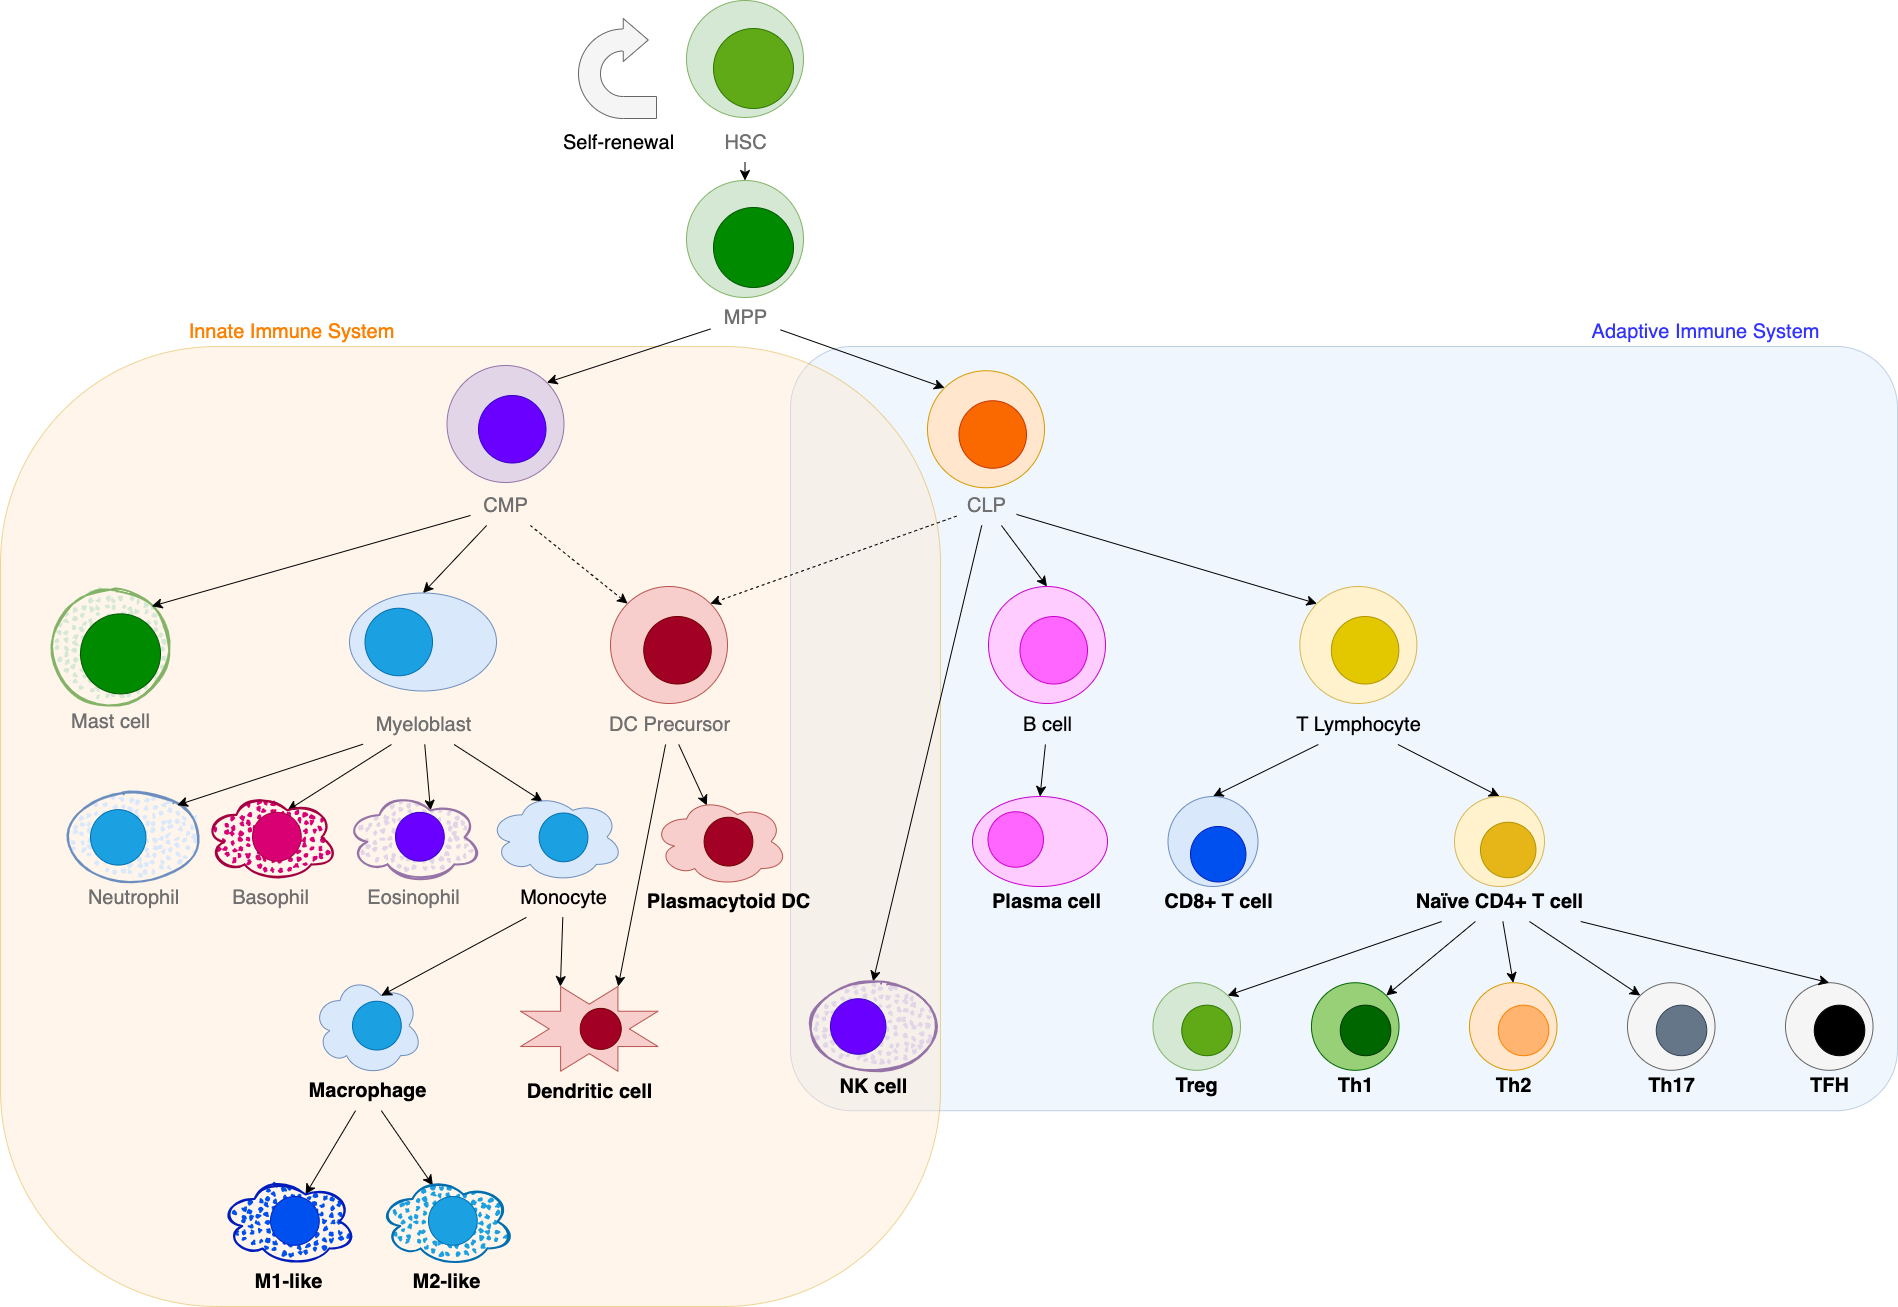
\includegraphics[width=\textwidth]{Figures/immunediff.png}
    \caption{\textbf{Lineage Tree representation of immune cell differentiation} Immune cells are derived from HSCs. HSCs then develop into multipotent progenitors (MPPs) in preparation for further differentiation. MPPs differentiate into common lymphoid and myeloid progenitors (CLPs and CMPs, respectively) before further development into more specified immune cell types within the adaptive and innate immune systems. Cells that are included in peripheral blood mononuclear cells (PBMCs) are in bold.}
    \label{fig:immune-cells}
\end{figure}

The immune system performs a wide range of functions within the body, including defense against pathogens and tumours and maintaining homeostasis of various body systems. In order to perform its role, the immune system relies on the coordinated efforts of complex immune response mechanisms. These mechanisms fall within either the innate immune system or the adaptive immune system and are executed by specialized immune cells each with their own specific role and function. The innate immune system is the body's first line of defense against common microorganisms. Innate immune responses are able to rapidly identify molecular patterns common to microbes and toxins foreign to the host through hard-wired responses encoded within the genes of the host's germ line \cite{immunediff}. For pathogens unable to be fought by the innate immune system, the adaptive immune system takes over by utilizing antigen specific recognition to target specific pathogens. These antigen specific cells are committed to memory through long-lived dormant cells that persist following a pathogen's first offense allowing the adaptive immune system to protect against subsequent reinfections from the same pathogen \cite{immunediff, Janeway2001}. Innate immune cells are comprised of innate lymphocytes such as natural killer (NK) cells and myeloid cells, including eosinophils, neutrophils, basophils, monocytes, and mast cells while adaptive immune cells are primarily made up of B Lymphocytes and T lymphocytes \cite{Klinke2019}.

There are over 80 different identified immune cell subsets each with specialized functions and characterized by specific cellular markers. Despite great heterogeneity amongst the various immune cell subsets, they are all commonly derived from hematopoietic stem cells (HSCs) in bone marrow. Through a multi-step differentiation process, immune cells commit to a cell lineage determined by various external and intrinsic factors including transcriptional reprogramming \cite{Wang2018}. Since the differentiation process contains a number of sequential specialization steps where the immune cells become increasingly distinct, the immune cell landscape is often referred to and depicted as a hierarchical lineage tree \cite{Klinke2019} (Fig. \ref{fig:immune-cells}). 

\subsection{Drivers of Immune Cell Differentiation}

\begin{figure}
    \centering
    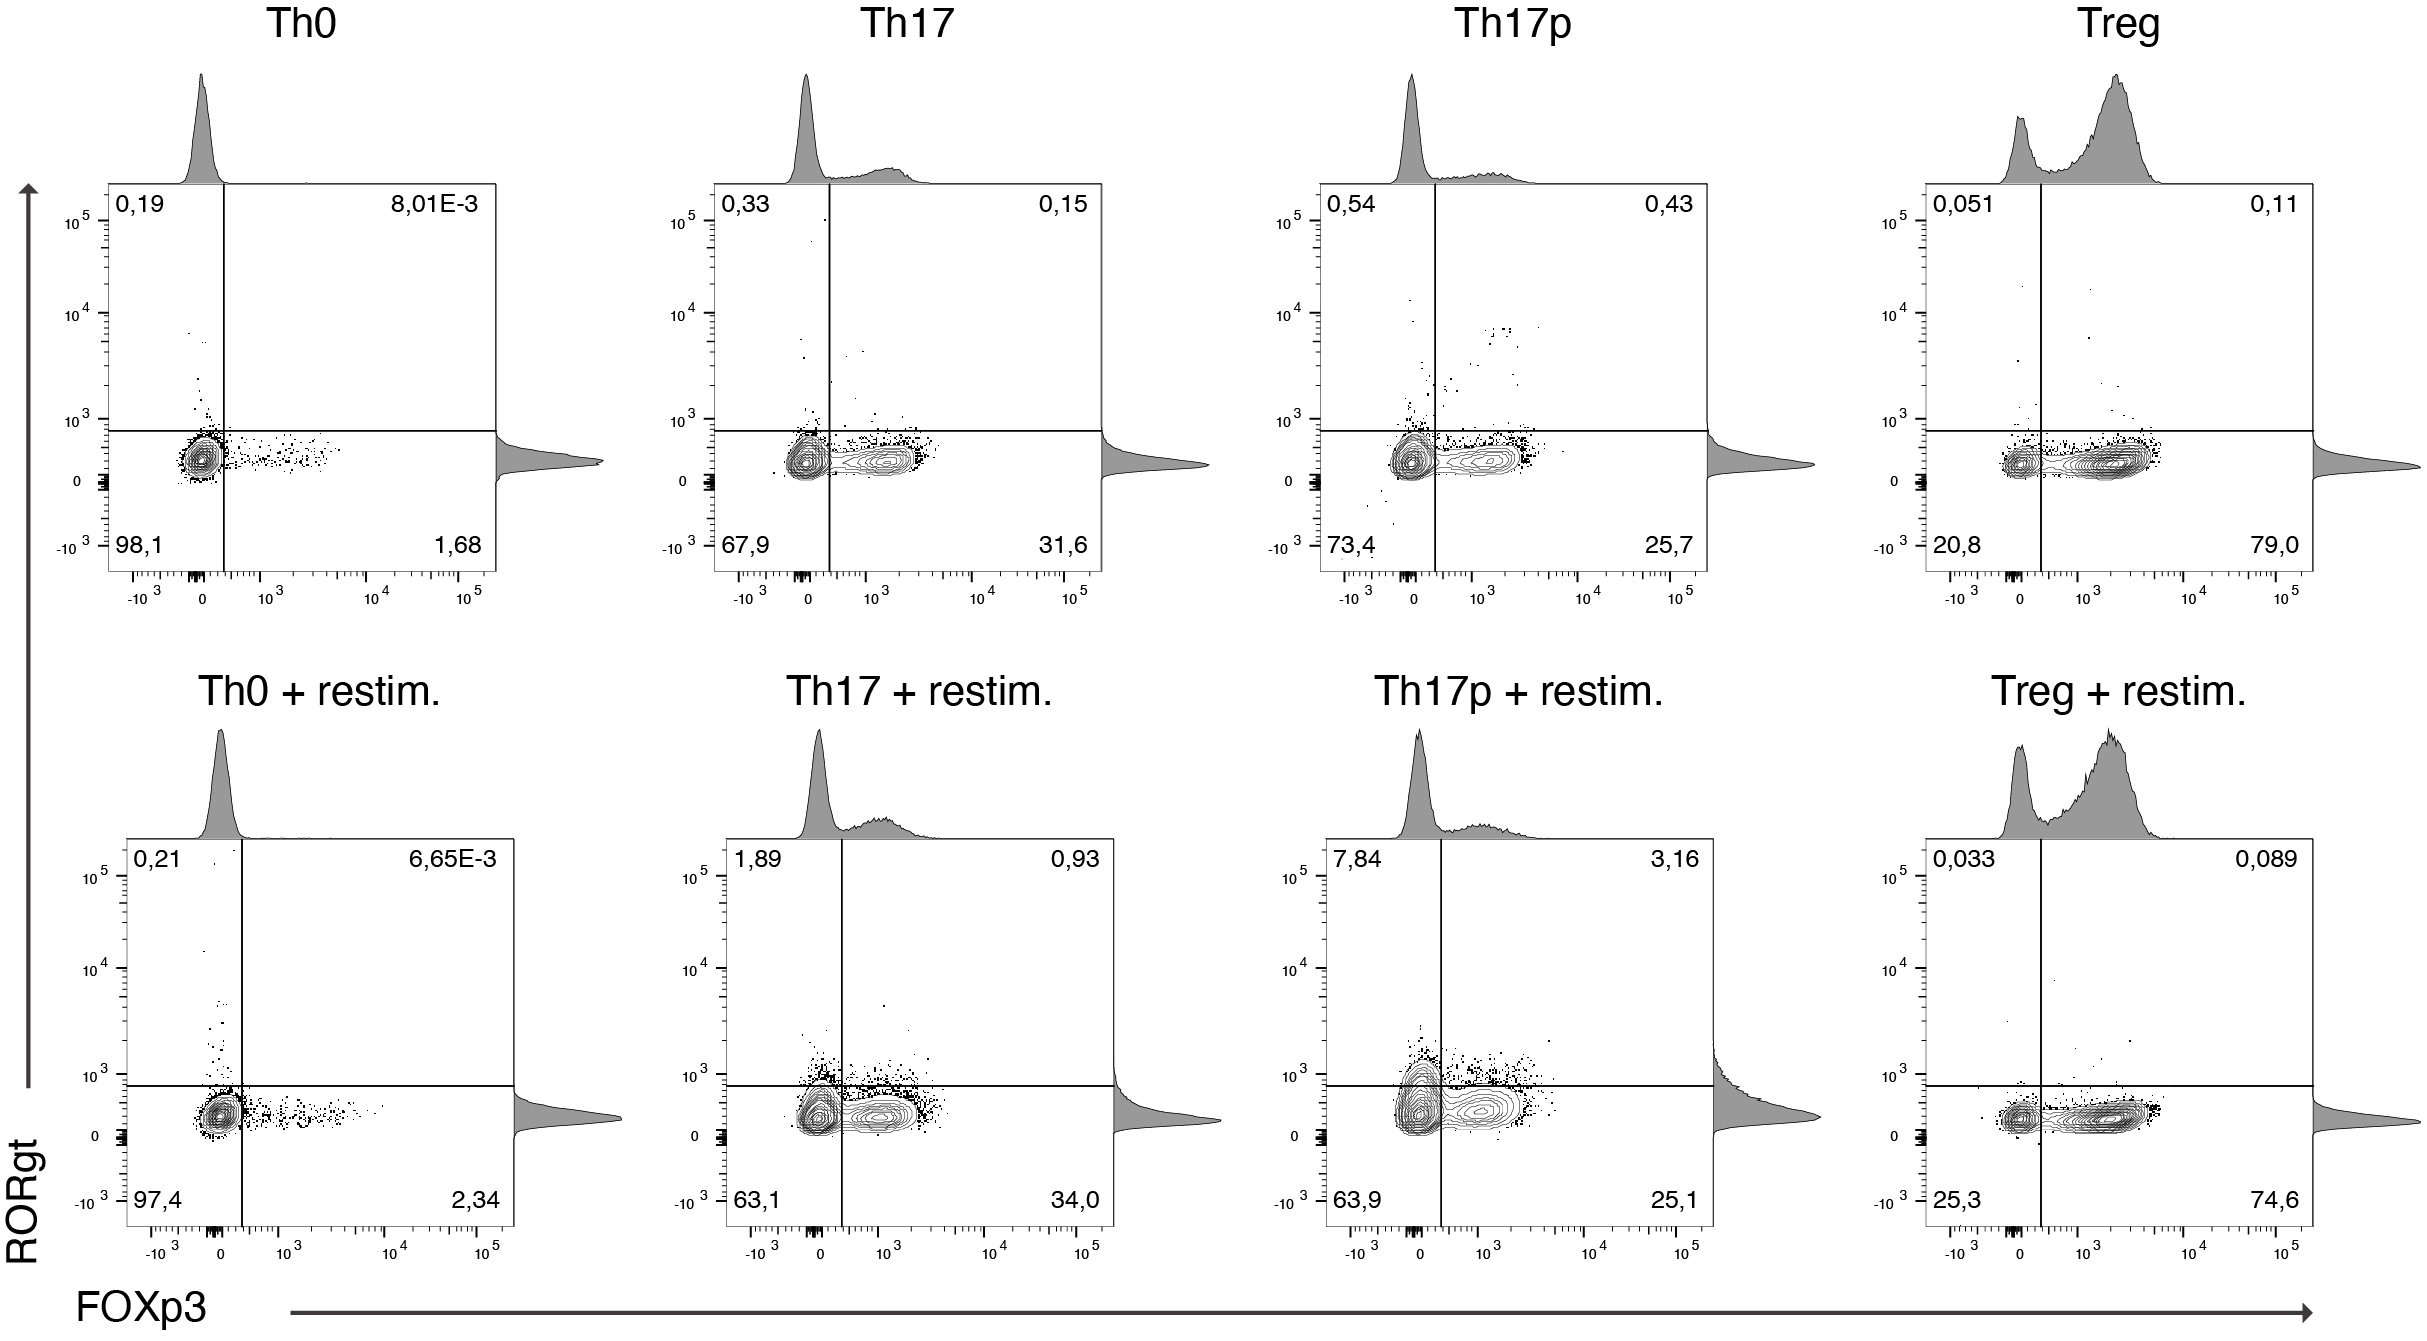
\includegraphics[width=\textwidth]{Figures/FOXp3_vs_RORgt.png}
    \caption{\textbf{\textit{In vitro} polarization of CD4+ T cells results in heterogeneous cell populations} Flow cytometry analysis performed on \textit{in vitro} polarized CD4+ T cells in Th0, Th17, pathogenic Th17 (Th17p), and Treg polarization conditions. Flow plots show protein expression of Foxp3 and Ror$\gamma$t \textemdash markers of Tregs and Th17, respectively \textemdash  in mouse CD4+ T cells.}
    \label{fig:CD4flow}
\end{figure}


\renewcommand{\arraystretch}{1.25}
\begin{sidewaystable}[]
\centering
\scalebox{0.8}{
\begin{tabular}{|c|c|c|c|c|c|c|c|c|c|}
\hline
\multicolumn{10}{|c|}{Treg} \\
 \hline
        Study & $\alpha$ CD3 & $\alpha$ CD28 & IL-2 & TGF-$\beta$ & TNF-$\alpha$ &  $\alpha$ IFN$\gamma$ & $\alpha$ IL-4 & $\alpha$ IL-12 & \textemdash\\
        \hline
        Field 2020 \cite{Field2020} & 5 $\mu$g/mL & 0.5 $\mu$g/mL & 100 U/mL & 5 ng/mL & \textemdash & 10 $\mu$g/mL & 10 $\mu$g/mL & 10 $\mu$g/mL & \textemdash\\
        Yang 2019 \cite{Yang2019} & beads & beads & 50 U/mL & 2 ng/mL & "accordingly" & \textemdash & \textemdash & \textemdash & \textemdash\\
        Xiao 2016 \cite{Xiao2016} & beads & beads & 25 U/mL & 3 ng/mL & \textemdash & \textemdash & \textemdash & \textemdash & \textemdash\\
        Thomas 2012 \cite{Thomas2012} & 1 $\mu$g/mL & 1 $\mu$g/mL & 20 U/mL & 5 ng/mL & \textemdash & \textemdash & \textemdash & \textemdash & \textemdash\\
        Jiang 2018 \cite{Jiang2018} & 5 $\mu$g/mL & 5 $\mu$g/mL & 10 U/mL & 2 ng/mL & \textemdash & \textemdash & \textemdash & \textemdash & \textemdash\\
        Pham 2014 \cite{Pham2014} & 2 $\mu$g/mL & 0.5 $\mu$g/mL & \textemdash & 2 ng/mL & \textemdash & \textemdash & \textemdash & 10 $\mu$g/mL & \textemdash\\
        Wagner 2021 \cite{Wagner2021} & 1 $\mu$g/mL & 1 $\mu$g/mL & \textemdash & 2 ng/mL & \textemdash & \textemdash & \textemdash & \textemdash & \textemdash\\
        Puleston 2021 \cite{Puleston2021} & 5 $\mu$g/mL & 2 $\mu$g/mL & 100 U/mL & 10 ng/mL & \textemdash & 4 $\mu$g/mL & 4 $\mu$g/mL & \textemdash & \textemdash\\
        \hline
 \multicolumn{10}{|c|}{Th17} \\
 \hline
        Study & $\alpha$ CD3 & $\alpha$ CD28 & IL-1$\beta$ & IL-2 & IL-6 & IL-23 & TGF-$\beta$ & $\alpha$ IFN$\gamma$ & $\alpha$ IL-4 \\
        \hline
        Field 2020 \cite{Field2020} & 5 $\mu$g/mL & 0.5 $\mu$g/mL & 10 $\mu$g/mL & 100 U/mL & 10 ng/mL & \textemdash & 5 ng/mL & 10 $\mu$g/mL & 10 $\mu$g/mL\\
        Yang 2019 \cite{Yang2019} & 1 $\mu$g/mL & 1 $\mu$g/mL & \textemdash & \textemdash & 10 ng/mL & \textemdash & 2 ng/mL & 5 $\mu$g/mL & 5 $\mu$g/mL\\ 
        Chen 2017 \cite{Chen2017} & beads & beads & \textemdash & 100 U/mL & 20 ng/mL & \textemdash & 20 ng/mL & \textemdash & \textemdash\\
        Thomas 2012 \cite{Thomas2012} & 1 $\mu$g/mL & 1 $\mu$g/mL & \textemdash & \textemdash & 10 ng/mL & 10 ng/mL & 1 ng/mL & 20 $\mu$g/mL & 20 $\mu$g/mL\\
        Jiang 2018 \cite{Jiang2018} & 5 $\mu$g/mL & 5 $\mu$g/mL & 10 ng/mL & \textemdash & 20 ng/mL & 50 ng/mL & 0.5 ng/mL & \textemdash & \textemdash\\
        Pham 2014 \cite{Pham2014} & 2 $\mu$g/mL & 0.5 $\mu$g/mL & 10 ng/mL & \textemdash & 100 ng/mL & 10 ng/mL & 2 ng/mL & 10 $\mu$g/mL & 10 $\mu$g/mL\\
        Wagner 2021 \cite{Wagner2021} & 1 $\mu$g/mL & 1 $\mu$g/mL & 20 ng/mL & \textemdash & 25 ng/mL & 20 ng/mL & \textemdash & \textemdash & \textemdash\\
        Gaublomme 2015 \cite{Gaublomme2015} & 2 $\mu$g/mL & 2 $\mu$g/mL & 20 ng/mL & \textemdash & 25 ng/mL & 20 ng/mL & 2 ng/mL & \textemdash & \textemdash\\
        Puleston 2021 \cite{Puleston2021} & 5 $\mu$g/mL & 2 $\mu$g/mL & 10 ng/mL & 100 U/mL & 5 ng/mL & \textemdash & 10 ng/mL & 10 $\mu$g/mL & 10 $\mu$g/mL\\
         \hline
    \end{tabular}
}
\caption{\textbf{Table summary of CD4+ polarization conditions} A meta-analysis of various studies with \textit{in vitro} CD4+ subset polarization condition protocols. Included are the polarization conditions for Tregs and Th17s across 10 studies. Units are presented as described in the original studies.}
\label{tab:CD4polarization}
\end{sidewaystable}

The process of immune cell differentiation is driven by cell signaling, a highly variable process influenced by a large number of factors including extracellular environment cytokine presence \cite{Sch_nherr_2000}, epigenetic mechanisms \cite{TURNER2020117}, cellular metabolism \cite{Pearce_2021, Chapman_2017}, transcription factors (TFs) \cite{Liu_2022}, host and host environment, and  microbiome \cite{ter_Horst_2016}. 

The complexity of immune cell differentiation is best exemplified through CD4+ helper T cell polarization. Naïve CD4+ T cells further differentiate into helper T cell subsets marked by distinct gene expression signatures, including cytokine expression, and require the presence of specific extracellular cytokines to polarize \cite{Zhang_2012}. In general, CD4+ T cell populations are heterogeneous following polarization as shown from flow cytometry analysis performed as described in \ref{cha:cd4diff} (Fig. \ref{fig:CD4flow}). Protein expression levels of Foxp3 and Ror$\gamma$t \textemdash regulatory markers of regulatory T cells (Tregs) and Th17 cells, respectively \textemdash are shown \cite{Rudensky_2011, Ivanov_2006}. Both Foxp3 and Ror$\gamma$t are induced in the presence of Tgf-$\beta$ and in the absence of a proinflammatory cytokine, such as IL-6, Foxp3 can inhibit Ror$\gamma$t function to drive towards a Treg phenotype \cite{Ziegler_2009}. The fate of CD4+ T cells is therefore highly influenced by the balance between these two proteins. In the Th17 and pathogenic Th17 (Th17p) polarization conditions without additional restimulation, only a very small subset of cells express Ror$\gamma$t, while a larger subset of cells express Foxp3, suggesting that cells are leaning towards a more suppressive phenotype rather than an effector Th17 phenotype. Cells expressing Ror$\gamma$t and therefore exhibiting a Th17 phenotype are only seen upon restimulation, though the population of suppressive Foxp3+Ror$\gamma$t- cells are still present in the same proportion (Fig.\ref{fig:CD4flow}).

Another factor that contributes to the uncertainty in the differentiation process of immune cells is plasticity between subsets, in the context of CD4+ T cells, it is the ability of a single cell to exhibit features of a number of T cell subsets simultaneously or over time \cite{Geginat_2014}.

A meta-analysis of a number of CD4+ polarization protocols summarized in Table \ref{tab:CD4polarization} and \ref{tab:CD4polarizationSupp} found a lack of consensus between researchers on the necessary extracellular cytokines and their quantities for subset polarization, particularly for Th17 polarization. This demonstrates that CD4+ T cell subset differentiation and immune cell differentiation in general is not entirely understood and there exists the need to further investigate their driving mechanisms and ways to capture the heterogeneous nature of these cell populations in a hierarchical manner. 

\newpage
\section{Pathogenesis of Systemic Lupus Erythematosus}

Systemic Lupus Erythematosus (SLE) is a complex, chronic autoimmune disease that affects approximately 3.17 million adults worldwide \cite{slepath, Tian_2022}. The disease presentation of SLE is highly heterogeneous between individuals and may affect any part of the body, but symptoms typically include fatigue, skin rashes, chronic inflammation, and fever. Many patients suffer from periods of disease exacerbations (flares) where worse or new symptoms are seen in one of more organ systems and a change or increase in treatment is required to suppress the overactive immune response \cite{Adamichou_2017}. Currently, there is no cure for SLE and therapeutic treatments of this disease severely affect the quality of life for patients.

Genetic factors play a crucial role in the development of SLE. About 90\% of SLE cases are female, however this sex difference remains poorly understood \cite{Furst_2012, Nusbaum_2020}. There is also a large discrepancy in the prevalence of SLE between races/ethnic backgrounds. East Asian and Hispanic/South American populations see the highest incidence rates of SLE \cite{Woo_2022}. The heritability of the disease is estimated to be around 44\% \cite{Kuo_2015}, but there has been great difficulty in pinpointing any specific genetic cause of disease manifestation \cite{Ceccarelli_2015}. Currently, there are over 60 confirmed genetic risk loci associated with SLE \cite{TERUEL2016161}. Many of the genes containing these loci are involved with regulatory functions within the innate and adaptive immune system. Genetic variants are suggested to have a regulatory effect on disease pathology since the majority of the SNPs found to be associated with SLE fall within non-coding regions of the gene. Despite the identification of many genetic risk loci, they are only able to explain a small fraction of the heritability of SLE. There are no genetic factors that have been found to be shared between all SLE patients due to the heterogeneous nature of disease manifestation \cite{Ceccarelli_2015}. 

There are a number of environmental factors that have been shown to be significantly associated with the presence of SLE. These factors include exposures such as air pollution, heavy metals, and ultraviolet radiation. Certain lifestyle choices also contribute to the development of SLE including alcohol consumption, cigarette smoking, sleep patterns, socioeconomic factors and stress, and diet and microbiome \cite{Woo_2022}. 

Epigenetic factors, innate and adaptive immunity, and inflammation have also been found to play a role in SLE pathogenesis and exist in the interface between environmental exposures and genetic risk factors and provide potential mechanisms to explain the effect of environmental exposures on disease. \cite{TERUEL2016161, Woo_2022}.


Several different risk factors are hypothesized to be associated with the development of SLE, but a direct cause of SLE remains unclear. The disease mechanism of SLE disease presentation is an area of ongoing investigation, but one known driver is the presence of autoreactive T and B cells, resulting in persistent inflammatory responses in the absence of pathogens. A better understanding of the cellular makeup of circulating immune cells in the body provides further insight into the causal mechanisms in SLE and other autoimmune disorders.

\subsection{Role of T Cells in SLE}

SLE pathogenesis is characterized by the presence of autoantibodies leading to chronic inflammation causing damage to tissues and organs. These autoantibodies are the result of defects in cellular apoptotic debris clearance, pro-inflammatory expression signatures in peripheral lymphocytes, and dysfunctional peripheral tolerance mechanisms \cite{slepath}. 

T cells contribute to SLE pathogenesis through the amplification of inflammation by secretion of pro-inflammatory cytokines. Additionally, the accumulation of autoreactive memory T cells results in sustaining disease over time.

CD4+ helper T cells signal to B cells through the production of cytokines. Abnormalities in the T cell receptor (TCR) leads to increased stimulation and results in aberrant activation of T cells \cite{Moulton_2015}. SLE patients have an imbalance of CD4+ T cell subsets. In peripheral blood CD4+ T cell populations, pro-inflammatory Th17s are overabundant, while suppressive Tregs are under-represented. As a result, there is an increased prevalence of the pro-inflammatory signaling cytokines IL-6 and IL-17 \cite{Talaat_2015}. Additionally, aberrant activation of PI3K/AKT/mTOR signal transduction leads to an increased accumulation of effector/memory T cells due to a resistance to activation-induced cell death \cite{Su_rez_Fueyo_2011}. Meanwhile, dysfunction in CD8+ T cells in SLE results in dampended cytotoxicity and results in increased risk of infection, potentially triggering autoimmunity \cite{Gravano_2013}. 

The significant role that T cells play in SLE pathogenesis, coupled with the lack of understanding behind the genetic drivers of SLE and the complex mechanisms of immune cell differentiation inspires the need to further investigate genomic mechanisms in immune cell subsets in patients with SLE.

\newpage
\section{Latent Representations of Biological Data} 

With the recent advancements of high-throughput screening (HTS) technologies, specifically single-cell RNA sequencing (scRNA-seq), knowledge of the molecular profiles of specific cell types has expanded. Since scRNA-seq data is high-dimensional, often capturing expression of tens of thousands of genes across thousands of cells, scalable and interpretable computational methods are necessary to perform sophisticated analysis of the data in order to uncover biological insights. One branch of these methods focuses on representing scRNA-seq data in a lower dimension latent space in a meaningful and interpretable way. Latent representations of biological data allows for further downstream analysis, such as cellular deconvolution using unsupervised clustering techniques \cite{Luecken_2019}. 

A key challenge in latent embedding of biological data is the inability to produce biologically interpretable results. Therefore extracting meaning from the data requires backfilling of information through manual annotation and analysis \cite{Kiselev_2019}.

\subsection{Deep-learning Methods for Biological Data} 

As datasets become increasingly large in the number of samples as well as dimensionality, there has been a shift towards deep-learning methods which are scalable and out-perform linear methods such as the iterative Harmony algorithm \cite{korsunsky2019fast} and non-negative matrix factorization (NMF) based methods such as LIGER \cite{liu2020jointly}.

Deep-learning based approaches for scRNA-seq most commonly use autoencoders, a type of artificial neural network, as a means to project high-dimensional data onto a low-dimensional latent space \cite{tschannen2018recent}. A number of recent methods utilize a variational autoencoder (VAE) \cite{Kingma2013-if}, a Bayesian method that relies on stochastic variational inference to efficiently scale to large datasets. These methods include single-cell variational inference (\texttt{scVI}) \cite{scvi} and single-cell VAE (\texttt{scVAE}) \cite{gronbech2020scvae}, the latter of which extends the VAE framework by using a Gaussian-mixture model as the prior distribution for latent variables over a Gaussian prior to learn cell clusters through a categorical latent variable.

Single-cell Embedded Topic Model (\texttt{scETM}) \cite{scETM} and Bayesian latent topic analysis with sparse association matrix (\texttt{BALSAM}) \cite{ZHANG2023100388}  are methods that make use of an embedded topic model (ETM) framework \cite{etm1}, an extension of VAE. In these methods, neural networks are used to encode scRNA-seq data into a latent topic space, while a generalized linear model (GLM) is used to decode latent embeddings back to the original gene expression space. As a result, these methods are able to simultaneously learn the parameters of the encoder neural networks and topic specific gene embeddings to create a highly interpretable latent space. 

\subsection{Methods to Model Cellular Hierarchies}

It has been suggested to use a tree-based reference structure to represent cell types as opposed to an atlas or periodic table-like classification system in order to better capture relationships between cell types \cite{treeref}. 

Therefore, a method that can embed scRNA-seq data in an interpretable latent space while learning a hierarchical tree-structure of data has the potential effectively identify cell clusters while providing insights into cellular relationships.

Hierarchical extensions to the topic modeling framework have been proposed where latent topics exist as nodes that lie in a tree structure. These methods include hierarchical latent Dirichlet allocation (\texttt{hLDA}) \cite{hlda} and tree-structured neural topic model (\texttt{TSNTM}) \cite{tree_etm}. \texttt{hLDA} uses a latent Dirichlet allocation (LDA) approach to represent topics in a hierarchical structure informed by a nested Chinese restaurant process prior. \texttt{TSNTM} makes use of autoencoding variational Bayes to efficiently construct a tree-structured latent topic space. Since the latent topic tree structures in these methods exist in an infinite tree space, meaning each node can have infinite child nodes, these models rely on Markov Chain Monte Carlo (MCMC) algorithms in order to simulate models over super-exponential space. Despite theoretical guarantees, these methods were not suitable for the purposes of scRNA-seq data due to the size of the data and the computational complexity associated with learning the topic tree structure. 

Another approach to model hierarchical representations of scRNA-seq data is to do \textit{post-hoc} construction of the tree-structured relationships between cells. \texttt{treeArches} \cite{sc_hier} aims to construct and extend a cell reference atlas and corresponding hierarchical classifier, relying on prior information from an existing cell atlas. \texttt{cellTree} infers tree-structured relationship hierarchies between individual cells based upon LDA latent representations and minimum spanning trees to construct the tree structure. These methods construct their relevant cellular tree representations after estimating their latent representations rather than learning the cellular hierarchies simultaneously with their latent representation. Additionally, \texttt{cellTree} only constructs the direct hierarchical relationships between individual cells, differing from the other modeling approaches which aim to define relationships between cell features through topics in order to represent hierarchical relationships.

\newpage
\section{Thesis Objectives and Hypothesis}
\subsection{Summary of rationale}

Immune cell differentiation is a complex biological process that remains an area for further investigation. The various immune cell subsets originate from a common HSC progenitor and follow a series of branching differentiation steps to reach maturity. As immune cells develop, they become more highly specific in cell features and function, resulting in greater dissimilarity with other immune subsets. The process results in a lineage tree structure between immune cell subsets where cells share hierarchical relationships with one another. Tree-structured latent modeling of HTS data, specifically scRNA-seq, has the potential to uncover insights into the cellular differentiation process, hierarchical relationships between immune cell subsets, and their shared and differing cellular features. Though a number of statistical latent models of scRNA-seq data exist, an efficient and effective tree-structured model for this purpose has yet to be shown.

Applications of such a model may also provide biological insights on the pathogenesis of disease driven by immune dysregulation such as SLE. SLE is a complex autoimmune disease that is characterized by chronic autoinflammation in one or many organ systems. One mechanism driving this autoinflammation is aberrant function and imbalance of peripheral blood lymphocytes. Though SLE is a heritable disease and through genome-wide association studies (GWAS) a number of risk loci have been identified, genetic mechanisms driving disease presentation are not well understood. 

\subsection{Thesis Aims and Outline}

In the work presented in this thesis, there are two main research aims that are addressed. 

First, I aim to develop a tree-structured topic model to represent immune cell subsets and their hierarchical relationships through shared and differing cellular features. In order for this model to be effective for these purposes and provide biological insight, I bear in mind the efficiency and interpretability of methods used. The second aim of this thesis is to apply the developed model to a scRNA-seq dataset from individuals with varying SLE disease conditions to show pathological differences in immune cell composition and identify specific genomic features that may play a role in SLE pathogenesis.

In Chapter \ref{cha:larch}, I propose \texttt{LaRCH} (\underline{La}tent \underline{R}epresentation of \underline{C}ellular \underline{H}ierarchies), a neural topic model with a underlying tree-structure representation of latent topics. This model is based on an ETM framework which allows for highly interpretable topic specific gene embeddings. Autoencoding variational Bayes is used to train the model to ensure computational efficiency. To demonstrate the efficacy of this model, I train LaRCH on a realistic simulated scRNA-seq dataset of immune cell subsets. Using this model I am able to reconstruct cellular hierarchies from their latent topic representations and perform further downstream analysis.

Chapter \ref{cha:sle} of this thesis shows the application of the LaRCH model on a large scRNA-seq dataset of PBMC samples from individuals with varying SLE disease statuses. I demonstrate the ability for LaRCH to deconvolve immune cell subtypes. Then through disease stratified analysis, I identify disease dependent differences in cell-type composition and cellular features. The interpretable model features of LaRCH are used to assign biological meaning to the latent topic space and identify potential genetic drivers of SLE disease mechanisms that inspire further experimental investigation.


%% Here we provide a short optional argument to \chapter[]{}.  This
%% optional argument will appear in the table of contents.  For long
%% titles, one should use this to give a single-line entry to the
%% table of contents.
\chapter{Tree Structured Topic Modeling}
\label{cha:larch}
To simultaneously learn a latent representation of cellular gene expression data and their hierarchical relationships, a tree-structured topic model is introduced. In this chapter, details of this model, referred to as a \underline{La}tent \underline{R}epresentation of \underline{C}ellular \underline{H}ierarchies (LaRCH), are shown along with the results of a trained model on a simulated single-cell gene expression dataset. 

\section[LaRCH]{LaRCH: \underline{La}tent \underline{R}epresentation of \underline{C}ellular \underline{H}ierarchies}

\begin{figure}
    \centering
    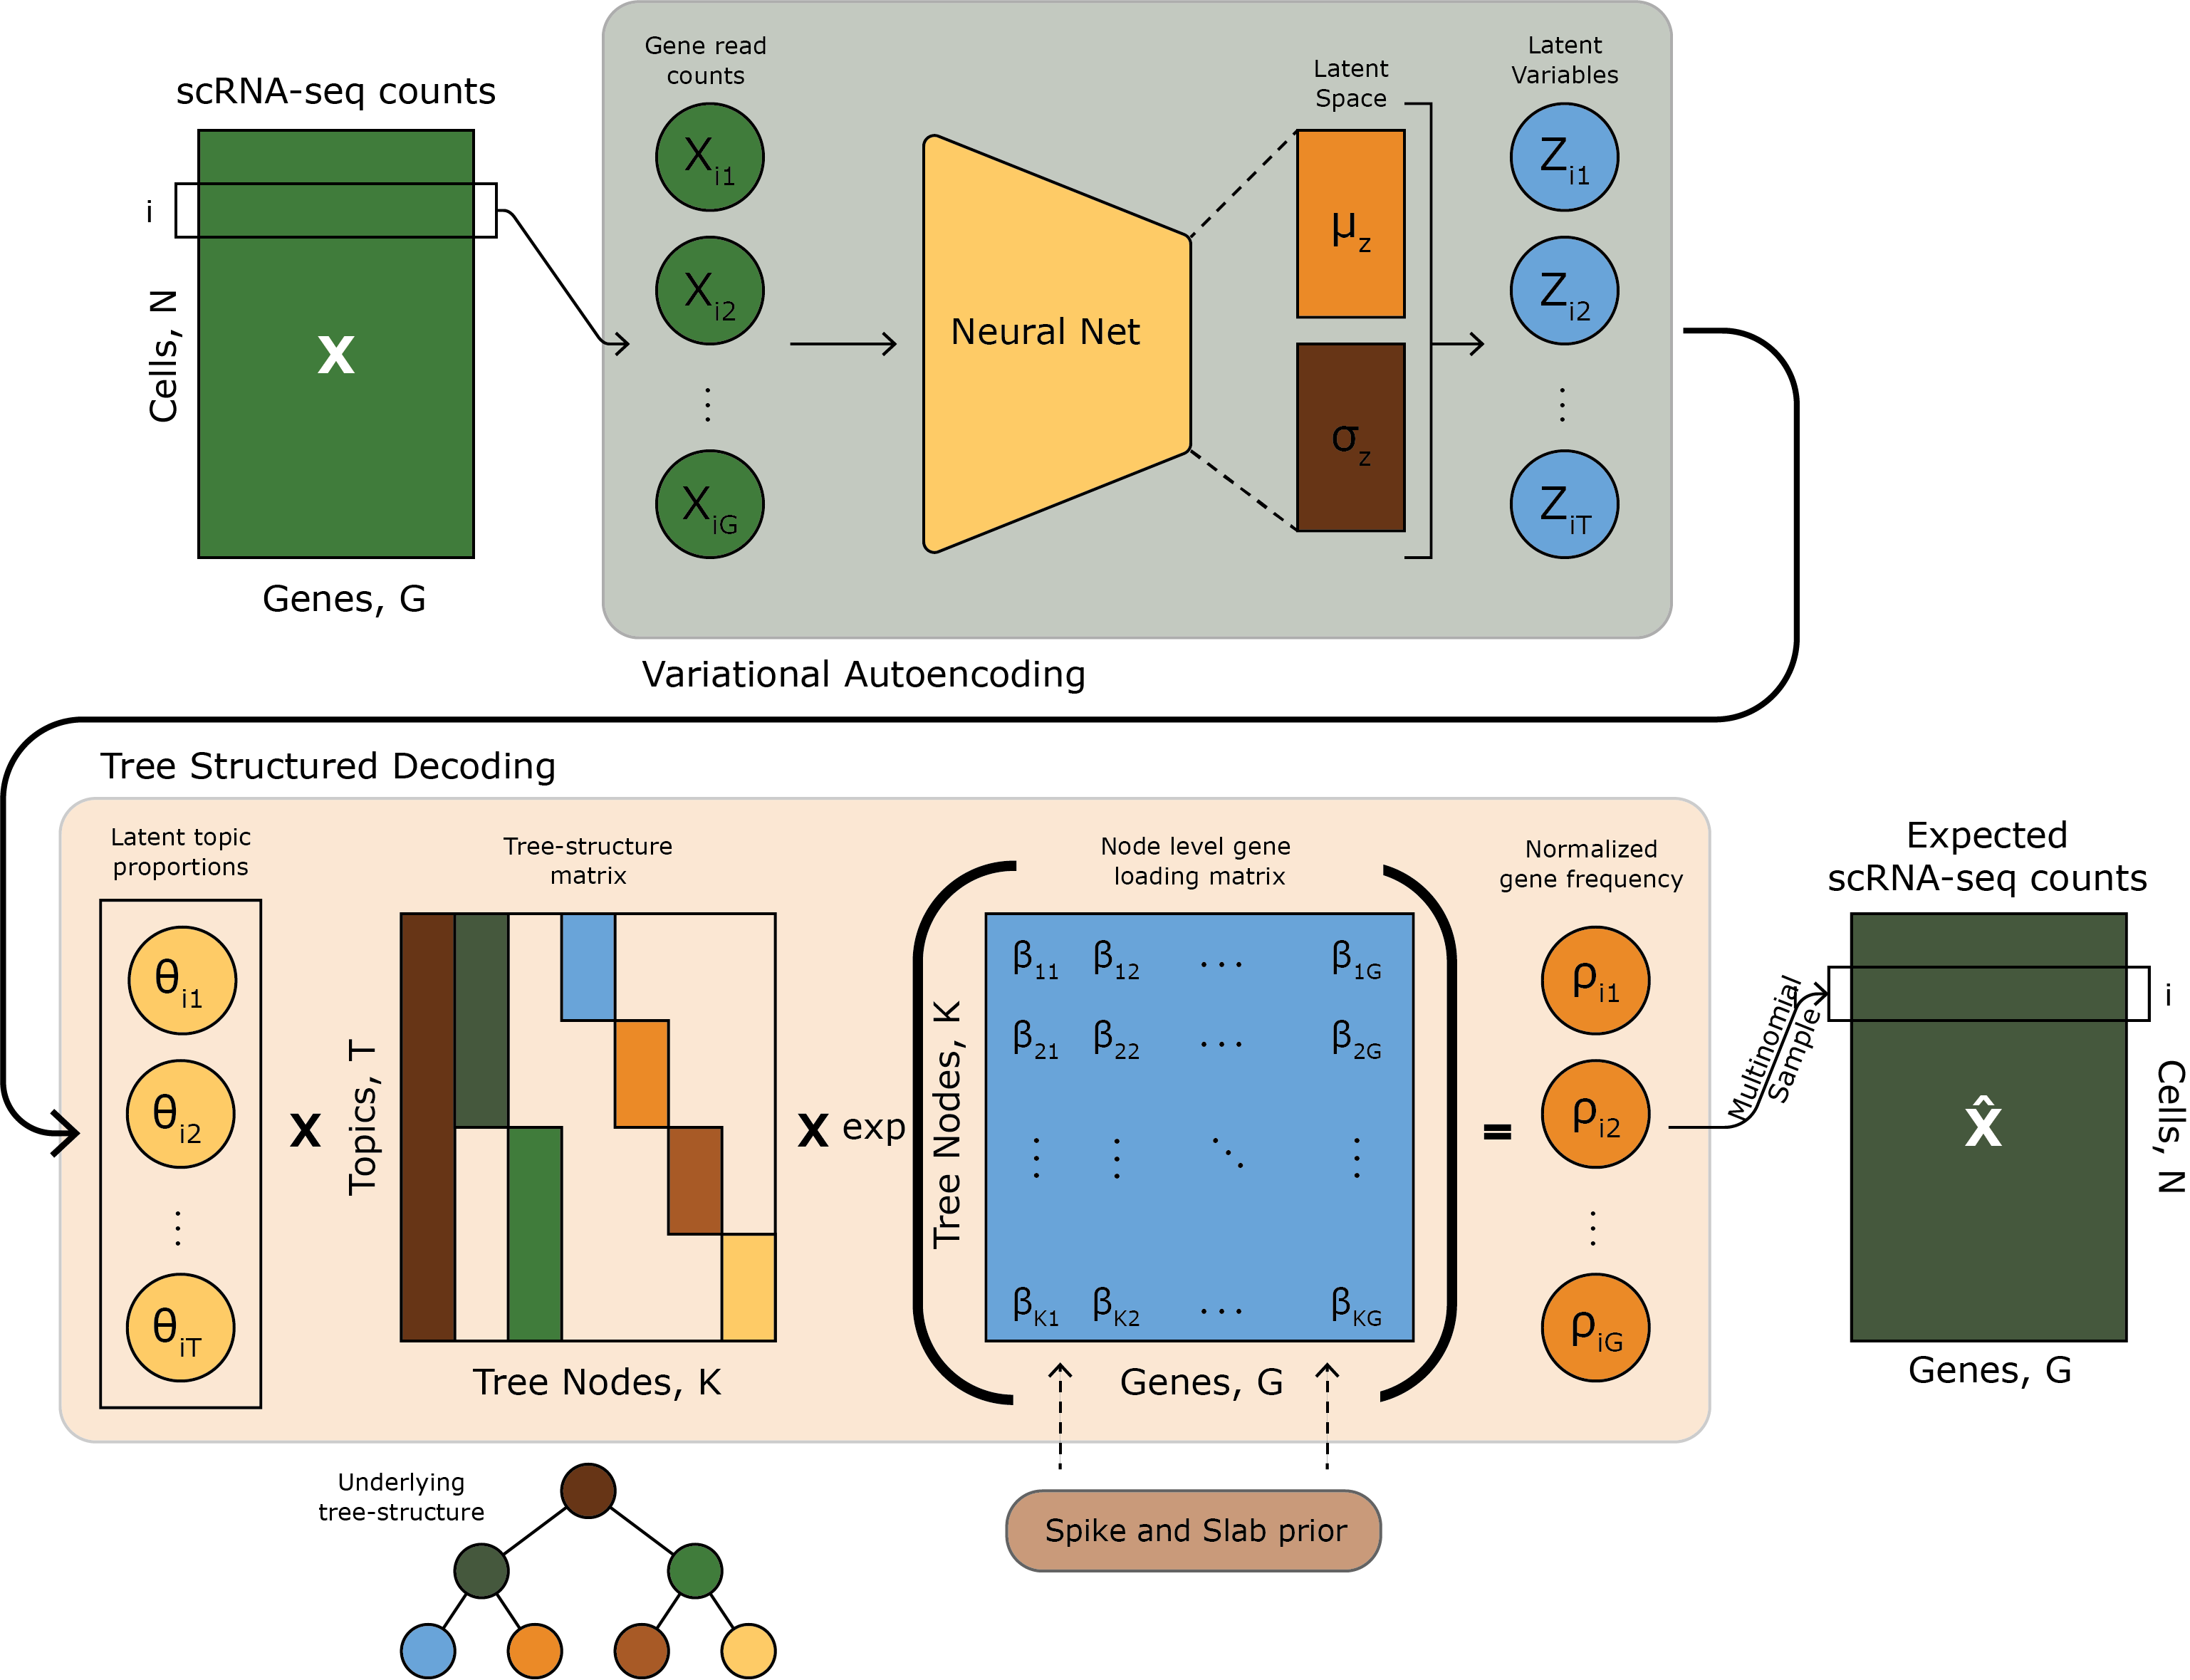
\includegraphics[width=\textwidth]{Figures/LaRCH_overview_0.png}
    \caption{\textbf{Overview of the LaRCH method} scRNA-seq data is encoded in latent features using a VAE. Original input data is then reconstructed through a generalized linear decoder containing the underlying PBT structure.}
    \label{fig:LaRCH}
\end{figure}

LaRCH uses an ETM \cite{etm1} approach built on a VAE \cite{Kingma2013-if,Kingma2014-pp,Kingma2015-mo} framework borrowed from neural network architectures with additional tree-node layer that aggregates sparse gene expression effects. Within a typical ETM, cells are represented as a mixture of latent topics each describing a gene expression profile of raw scRNA-seq count data. LaRCH introduces an additional layer of latent nodes that lie within a PBT structure (Fig. \ref{fig:LaRCH}). As a result, cells are viewed as a mixture of latent topics, each corresponding to a summation of tree nodes along a path from the root node to a given leaf node of the underlying tree. From this structure, it is inferred that topics that lie in close proximity on the tree share a number of properties while those further apart are also more distant in their features. As a more specific example, two topics corresponding to paths terminating at sibling leaf nodes would share all features captured in their common parent nodes, only diverging at the last branching point in their paths. Cells within these two topics would be said to share a large number of gene expression features represented by their shared parent nodes in their topic paths. 

The LaRCH model is comprised of an encoder and decoder component. The encoder transforms raw single-cell gene expression count data into the latent topic space through a neural net. In this model, rather than choosing the number of latent topics to represent the data, the depth of the latent-node tree $D$ is pre-determined, therefore the resulting number of total latent tree nodes is $2^D - 1$, and the latent topic space that the gene count data is transformed to is of dimension $2^{D-1}$. This latent representation is then converted to a topic proportion representation using the softmax function. 

Where LaRCH differs from a typical ETM lies in the decoder. The decoder contains a gene embedding matrix $\beta$ for each tree node as model parameters. Gene embedding values represent relative gene expression frequencies for a given tree node. Additionally, the tree-structured relationships at the topic level are represented mathematically using a structural matrix. The learned gene embedding matrix, structural matrix, and inferred topic proportions are passed to a GLM to estimate the cell specific gene frequencies for each data point. These gene frequencies are then used to compute likelihood values for expected gene counts.


\subsection{Data generative scheme}

To apply the LaRCH topic model, each cell is treated as a document, the set of genes in the dataset as the vocabulary of size $G$, and each scRNA-seq read as a token of a gene from the vocabulary. Each cell $i$ of $N$ cells is then represented as a mixture of $T$ latent topics in our model. 

In a classic ETM, each topic has a corresponding distribution over the gene space $\beta \in \mathbb{R}^{T \times G}$ \cite{etm1}. This is altered by introducing an additional latent tree node layer to the embedding process. $K$ latent nodes lie in a PBT structure of depth $D$, where $K = 2^D - 1$. Each of the $T$ latent topics, where $T = 2^{D-1}$, corresponds to a path from the root node to a leaf node of the PBT. Each tree node now has an embedding over the gene space $\beta \in \mathbb{R}^{K \times V}$ and each topic also has an embedding made up of the tree nodes along its corresponding path $\bar{\beta} =A\exp(\beta)$, where $A$ is a $T \times K$ matrix that captures the PBT structure. From this, two topics with similar paths in the tree-structured node will share gene embeddings while the paths are identical, then differ once the paths split. 

The formal data-generating process for each cell $i$, where $i = 1, \dots, N$, in the scRNA-seq dataset is:
\begin{enumerate}
    \item Draw latent topic proportion $\theta_i$ for cell $i$ from:
    \begin{equation}
        \theta_i = \text{softmax}(z_i) = \frac{\exp(z_{it})}{\sum_{t = 1}^T \exp(z_{it})}, z_i \sim \mathcal{N}(0, \textbf{I})
    \end{equation}
    \item Determine the categorical distribution $\rho_i$ of genes for cell $i$ based on $\theta_i$:
    \begin{equation}
        \tilde{\rho}_i = \theta_iA\exp(\beta), \rho_i \sim \text{Dirichlet}(\tilde{\rho}_{i1}, \tilde{\rho}_{i2}, \dots, \tilde{\rho}_{iG})
    \end{equation}
    \item Draw gene $g$ for each read of a cell from a multinomial distribution to give total gene counts over $R$ reads:
    \begin{equation}
        X_i|\rho_i \sim \text{Multinomial}(R, \rho_i)
    \end{equation}
    This gives the probability distribution: 
    \begin{equation*}
        p(X_i|\rho_i)\propto \prod_{g\in G} \rho_{ig}^{X_{ig}}
    \end{equation*}
    Where $\sum_{g}\rho_{ig} = 1$ for all $i \in 1, \dots, N$ and $\rho_{ig} \geq 0$ for all cells $i$ and genes $g \in [G]$
\end{enumerate}

Gene expression counts are said to follow independent multinomial probabilities (a bag of words assumption). Compared to other deep learning methods based on Poisson, Negative Binomial, and Gaussian distributions, a multinomial likelihood better preserves scale-invariant properties mitigating batch effects on the trained model. 

Here $z_i$ is the $1 \times T$ latent topic embedding of cell $i$, $\theta_i$ is the $1 \times T$ topic mixture of cell $i$ where $\sum_{t = 1}^T\theta_{i,t} = 1$, $\beta$ is a $K \times G$ gene embedding matrix for latent nodes, $A$ is a $T \times K$ matrix representing the tree-structure of nodes, $\rho_i$ is the $1 \times G$ cell specific distribution of gene reads, and $X_i$ is the $1 \times G$ count vector of genes. 

\subsection{Informing Model Parameters Through Bayesian Priors}
\subsubsection{A Dirichlet Prior to Inform Multinomial Sampling}

A Dirichlet prior is introduced to inform the categorical distribution of genes for each given cell, $\rho_i \sim \text{Dir}(\tilde{\rho}_i)$. This allows for direct transformation from the parameters $\tilde{\rho}$ to a distribution vector from which to sample multinomial values. The Dirichlet parameters are formulated as a GLM,
\begin{equation*}
    \tilde{\rho}_{ig} = \sum_{t = 1}^T\theta_{it}\sum_{k = 1}^K A_{tk}\exp(\beta_{kg}) - Db_g
\end{equation*}

This GLM captures the additive effects of nodes within each topic and the proportional additive effects of topics within each cell on the relative gene expression profile. 

An additional gene-specific bias parameter $b_g$ is used to represent invariant effects across all latent nodes. Since this parameter is present for each node, at the topic level, the additive effect of this parameter is $Db_g$. This is a free parameter without any specified prior distribution.
 
Since the multinomial and Dirichlet distribution share a conjugate relationship, the composite variable $\rho$ can be integrated out to obtain the posterior predictive likelihood, 
\begin{align*}
    p(x_i | \theta_i, \{\beta_{kg}\}, \{b_g\}) &= \int p(x_i | \rho_i)p(\rho_i | \theta_i, \{\beta_{kg}\}, \{b_g\})d\rho_i\\
    &= \frac{\Gamma(\sum_g \tilde{\rho}_{ig})\Gamma(\sum_g X_{ig} + 1)}{\Gamma(\sum_g \tilde{\rho}_{ig} + X_{ig})}\prod_g\frac{\Gamma(X_{ig} + \tilde{\rho}_{ig})}{\Gamma(\tilde{\rho}_{ig}) \Gamma(X_{ig} + 1)}\\
    &\propto \frac{\Gamma(\sum_g X_{ig} + 1)}{\prod_g \Gamma(X_{ig} + 1)}\frac{\prod_g\Gamma(X_{ig} + \tilde{\rho}_{ig})}{\Gamma(\sum_g \tilde{\rho}_{ig} + X_{ig})},
\end{align*}

where $\tilde{\rho}_{ig} = \sum_{t = 1}^T\theta_{it}\sum_{k = 1}^K A_{tk}\exp(\beta_{kg}) - Db_g$, and $\Gamma(\cdot)$ is the Euler's gamma function.

\subsubsection{Using a Bayesian Prior to Induce Model Sparsity}
Since scRNA-seq data is typically sparse with only a few non-zero features and shared expression of many highly expressed genes in general, the trained model used to represent this data should reflect this. To induce sparsity and increase interpretability in the gene embedding model parameters, $\beta$, a Bayesian spike-and-slab distribution prior \cite{Mitchell1988-yj} is used to inform their values. Within the spike-and-slab prior distribution, it is assumed that the majority of gene-embedding values $\beta_{kg}$ are statistically zero with some probability $1-\pi$. This concentration around zero is called the "spike" component of the distribution. The "slab" portion of the distribution is explained by a normal distribution centred around 0 with variance $\tau$. 
\begin{equation}
    \beta_{kg} \sim \pi \mathcal{N}(0,\tau) + (1 - \pi)\delta_0 (\beta_{kg})
\end{equation}




\subsection{Variational Inference}
Since exact inference of the posterior probability of latent topics $p(\theta_i | x_i)$ is computationally intractable in high dimensional spaces, stochastic variational inference is used as a scalable approach to finding approximate distributions \cite{Kingma2013-if}. 

The variable estimation scheme as described in Kingma \textit{et al.} is used\cite{Kingma2013-if}. In this reparameterization technique, latent variable inference is cast into an optimization problem in a deep belief network. This can then be solved using back-propagation steps with respect to model parameters. 

Variational inference is used to estimate two sets of parameters, the cell-specific latent topic proportions $q(\theta_n)$ and the node-specific gene-embedding parameters $q(\beta_{kg})$. For each set of parameters, the minimized Kullbeck-Leibler (KL) divergence is used to approximate the actual data likelihood probability. This is equivalent to maximizing the evidence lower bound (ELBO) for the total data likelihood, $\mathcal{L}$.

\begin{align}
    \ln p(\textbf{X}) & \geq 
    \mathbb{E}_q \left[\ln \frac{ p(\textbf{X}, \Theta, \beta)}{q(\Theta, \beta | \phi, \xi)}\right] \triangleq \mathcal{L}\\
    \sum_{i\in [N]}\int_{\theta, \beta}p(x_i, \theta_i, \beta) d\theta_i d\beta_i & \geq\mathbb{E}_q\left[\ln \frac{p(\textbf{X} | \Theta, \beta) p(\theta_i) p(\beta | \pi, \tau)}{q(\Theta | \phi)q(\beta | \xi)}\right]    \\
     \label{ELBO} = \mathbb{E}_q\left[\sum_{i\in [N]}\ln p(x_i | \theta_i, \beta)\right] &+ \mathbb{E}_q \left[\sum_{i\in [N]} \ln \frac{p(\theta_i)p(\beta | \pi, \tau)}{q(\theta_i|\phi)q(\beta|\xi)}\right] \\ 
     = \mathbb{E}_q \left[\sum_{i\in [N]}\ln p(x_i | \theta_i, \beta)\right] &+ \sum_{i\in [N]} \left[ \mathbb{E}_q \left[\ln \frac{p(\theta_i)}{q(\theta_i|\phi)}\right] + \mathbb{E}_q \left[\ln \frac{p(\beta | \pi, \tau)}{q(\beta|\xi)}\right]\right]\\
     \label{KL-elbo} = \mathbb{E}_q \left[\sum_{i\in [N]}\ln p(x_i | \theta_i, \beta)\right] &- \sum_{i\in [N]} \left[\text{D}_{\text{KL}}(q_\theta \parallel p_\theta) + \text{D}_{\text{KL}} (q_\beta \parallel p_\beta)\right]
\end{align}

Where $\phi$ and $\xi$ are used to denote all parameters of the latent state or parameter distributions, $\pi$ and $\tau$ are the probability of inclusion and variance parameters, respectively. Stochastic gradient steps with respect to the variational parameters $\phi$ and $\xi$ are taken in the variational inference algorithm, optimizing the ELBO objective (\ref{ELBO}) in order to find approximate posterior distributions. Variational inference is implemented in \texttt{Pytorch} using \texttt{torch.autograd} \cite{pytorch, pytorchdiff} to calculate gradients. 

\subsubsection{Approximation of latent topic proportions $\theta$}

Latent topic proportions, $\theta$ cannot be exactly evaluated, so are instead approximated by summing over the posterior predictive log-likelihood using sampled instances of $\theta^{(s)}$ and $\beta^{(s)}$ for each minibatch sample $s \in [S]$

\begin{equation}
    \mathbb{E}_q \left[\sum_{i\in [N]} \ln p(x_i|\theta_i, \beta)\right] \approx \frac{1}{S} \sum_{s \in [S]} \ln p(x_s | \theta^{(s)}, \beta^{(s)})
\end{equation}

The mean $\mu$ and variance $\sigma$ functions for latent variable inference are parameterized in the encoder model which takes the original high-dimensional scRNA-seq data $x$. $\theta^{(s)}$ is then posteriorly sampled using the reparameterization trick of the Logistic Normal distribution as follows: 
\begin{enumerate}
    \item Sample random error $\epsilon_s \sim \mathcal{N}(0,1)$
    \item Reparameterize latent topic variables $z_s \leftarrow \mu(x_s) + \sigma(x_s) \circ \epsilon_s$
    \item Transform latent variables to latent topic proportions: \\$\theta_t^{(s)} \leftarrow \frac{\exp(Z_{st})}{\sum_{j = 1}^T \exp(Z_{sj})}$
\end{enumerate}

Assuming $z_s \sim \mathcal{N}(0, I)$ \textit{a priori} for all $s$, the corresponding variational parameters $\phi \equiv (\mu, \sigma)$ is used to derive the KL divergence between the prior and variational distributions as the second term of (\ref{KL-elbo}): 
\begin{equation}
    \mathbb{E}_q \left[\ln \frac{q(Z_{st} | \phi)}{p(Z_{st})}\right] = \text{D}_{\text{KL}}(q_\theta \parallel p_\theta) = \sum_{t = 1}^T \frac{1}{2}[\mu_{st}^2 + \sigma_{st}^2 - \ln \sigma_{st}^2 - 1]
\end{equation}

\subsubsection{Approximation of global spike-and-slab parameters $\beta$}

Fully-factored spike-and-slab distributions are used as variational distributions for node-specific gene embedding parameters, $\beta_{kg}$, to derive the final term of (\ref{KL-elbo}), the negative KL loss of the global parameters, $\beta$.

When $\beta_{kg}$ is 'on', denoted by a latent indicator variable $h_{kg} = 1$ with probability $\alpha_{kg}$, $\beta_{tg}$ is parameterized by a Gaussian distribution:

\begin{equation*}
    q(\beta_{kg}| h_tg =1) = \mathcal{N}\left(\mu_{kg}^\beta, \nu_{kg}^\beta\right)
\end{equation*}

with probability $\alpha_{kg} \triangleq p(h_{kg} = 1)$; otherwise, $\beta_{kg}$ is set to zero:
\begin{equation*}
    q(\beta_{kg}|h_{kg} = 0) = \delta_0(\beta_{kg})
\end{equation*}

with probability $1-\alpha_{kg}$.

From the variational parameters $\xi \equiv (\alpha, \mu, \nu)$, the variational distribution is characterized as:

\begin{equation}
    q(\beta_{kg}) = \prod_{g\in G} \alpha_{kg}\mathcal{N}(\mu_{kg}, \nu_{kg})
\end{equation}

with 

\begin{equation}
    \mathbb{E}_q[\beta_{kg}] = \alpha_{kg}\mu_{kg} \label{eq:betahat_est} 
\end{equation}
\begin{equation}
    \mathbb{V}_q[\beta_{kg}] = \alpha_{kg}(1-\alpha_{kg})\mu_{kg}^2 + \alpha_{kg}\nu_{kg} \label{eq:betahat_var}
\end{equation}

This give the full reparameterization of $\beta$ as follows:
\begin{enumerate}
    \item Sample random error $\epsilon\sim\mathcal{N}(0,1)$
    \item Reparameterize node-specific gene embedding values $\beta_{kg} \leftarrow \mathbb{E}_q[\beta_{kg}] + \mathbb{V}_q[\beta_{kg}]^{\frac{1}{2}}*\epsilon - b_g$
\end{enumerate}

Assuming $h_{kg} = 1$ with probability $\pi_0$ and $\beta|h=1 \sim \mathcal{N}(0, \tau_0)$ \textit{a priori}, the KL loss is derived as follows:

\begin{align}
    -D_{KL}(q||p) = &\frac{\alpha_{kg}}{2}\left[1 + \ln \frac{\nu_{kg}}{\tau_0} - \frac{1}{\tau_0}(\mu_{kg}^2 + \nu_{kg})\right] + \\
    &\left[\alpha_{kg}\ln\frac{\pi_0}{\alpha_{kg}} + (1 - \alpha_{kg}\ln\left(\frac{1 - \pi_0}{1 - \alpha_{kg}}\right)\right]
\end{align}

\subsection{Model Implementation}

LaRCH is implemented in Python, using the \texttt{PyTorch} machine learning library \cite{pytorch}. The model makes use of the \texttt{torch.autograd} function to perform stochastic variaitonal inference \cite{pytorchdiff}.

\subsection{Code Availability}

Code containing the most up-to-date version of the \texttt{LaRCH} package, documentation, data simulation scripts of the simulation scheme presented in \ref{cha:datasim}, and a model pipeline can be found at \url{https://github.com/causalpathlab/LaRCH}.

\newpage
\section[Modeling Simulated Data]{Modeling Simulated Data from Bulk RNA-seq Expression}

Simulated single-cell gene expression data of immune cell subtypes was generated based on bulk-sequenced gene expression profiles from the Database of Immune Cell Expression \cite{DICE1}. This generated data was then used to train an instance of the LaRCH model in order to test its efficacy. 

\subsection{Bulk Gene Expression Profile Generation}
The DICE database bulk gene expression profiles are measured from human PBMCs obtained from leukapheresis samples. Immune cell types of interest were isolated from PBMC samples prior to total RNA isolation using fluorescence-activated cell sorting (FACS) based on fluorescent antibody staining either directly or following pre-enrichment using human B cell or memory CD4+ T cell isolation kits for B cell and CD4+ T cell samples, respectively \cite{DICE1}. FACS-sorted naive CD4+ and CD8+ T cells underwent an additional \textit{ex vivo} CD3/CD28 activation step for their respective activation conditions. 

Total RNA purified from FACS-sorted cell samples was then bulk sequenced and mapped against the hg19 reference genome and the GENCODE annotation v19 as the gene reference model. The expression profiles used in the data simulation scheme are expressed in transcripts per million (TPM) units. A full outline of the sample processing and RNA sequencing steps for this data can be found in Schmiedel et al. \cite{DICE1}.



\subsection{Data Simulation Scheme}
\label{cha:datasim}
The simulation scheme used to generate realistic single-cell gene expression data for $N$ cells is as follows:
\begin{enumerate}
    \item Determine the desired noise proportion $\rho$ and total transcript count $R$. $\rho$ represents the proportion of the gene expression distribution for a given 'cell' that is explained by a null distribution, $\pi_0$, common to all cell types. $1-\rho$ then represents the proportion of the gene expression distribution for a given 'cell' that is explained by a cell-type specific distribution $\hat{\pi}_t$. 
    \item Determine the null and cell type-specific gene expression distributions, $\pi_0$ and $\hat{\pi}$, respectively:
    \begin{equation}
        \pi_0 \sim \text{Dirichlet}(1, \dots, 1), 
        \hat{\pi}_{tg} = \frac{\text{bulk}_{tg}}{\sum_g \text{bulk}_{tg}}
    \end{equation}
    Where bulk$_{tg}$ is the bulk expression profile for cell type $t$ at gene $g$.
    \item Determine a cell type distribution across the simulated data sample, $m$:
    \begin{equation*}
        m \sim \text{Dirichlet}(1,\dots, 1)
    \end{equation*}
    \item For a cell $i$, where $i = 1, \dots, N$:
    \begin{enumerate}
        \item Randomly sample cell type $t_i$ according to $t_i \sim \text{Categorical}(m)$
        \item Gene expression distribution for cell type $t_i$:
        \begin{equation}
            \pi_{t_i} = (1 - \rho) * \hat{\pi}_{t_i} + \rho * \pi_0
        \end{equation}
        \item Sample gene transcript counts $X_i$:
        \begin{equation*}
            X_i \sim \text{Multinomial}(R, \pi_t)
        \end{equation*}
    \end{enumerate}
\end{enumerate}


\begin{figure}
    \centering
    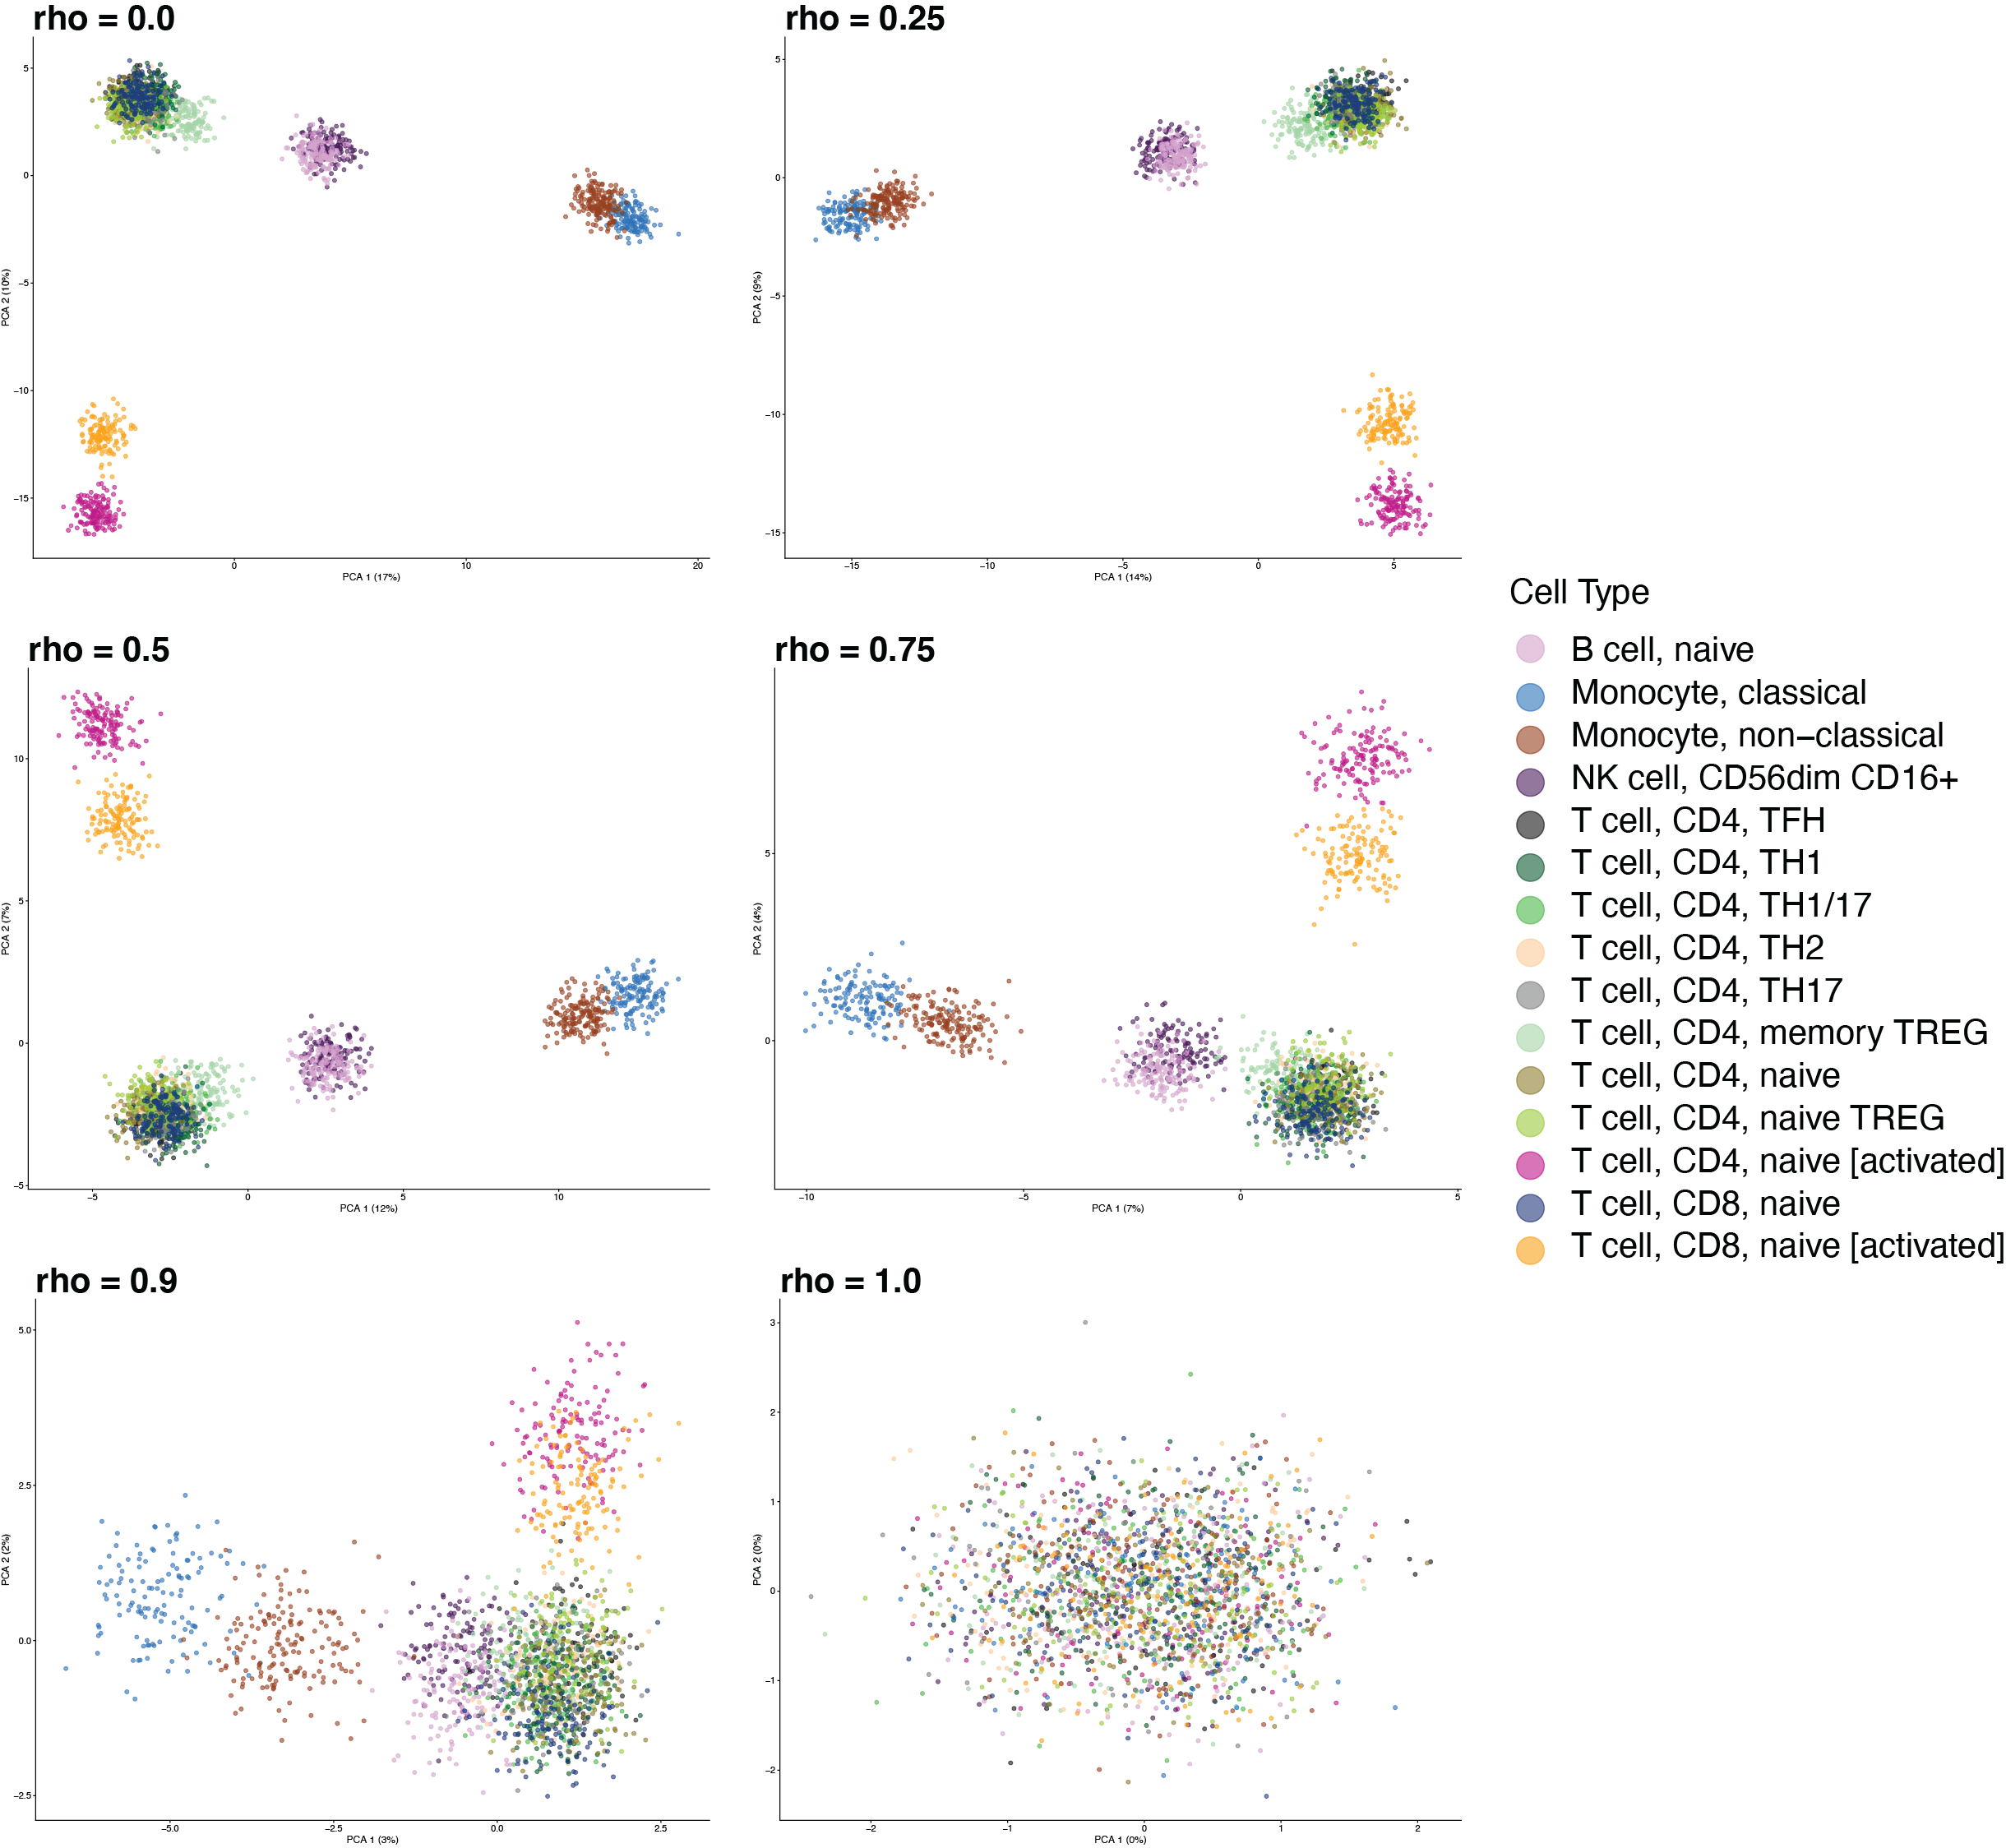
\includegraphics[width=\textwidth]{Figures/sim_data_PCA.png}
    \caption{\textbf{Simulated scRNA-seq datasets exhibit realistic distribution of expression patterns across various noise levels} Shown are the plots of first two PCs for generated immune cell scRNA-seq datasets from the simulation scheme. Datasets generated using various noise proportions $\rho =$ \{0.0, 0.25, 0.5, 0.75, 0.9, 1.0\} are shown and coloured by cell type.}
    \label{fig:ct-pca}
\end{figure}
\subsection{Resulting Simulated Data}
Pseudo scRNA-seq datasets of $N = 2000$ cells and total transcript count $R = 2500$ with varying noise proportions $\rho$ are obtained from the simulation scheme (Fig. \ref{fig:ct-pca}). Total gene count value $R$ is chosen to approximate UMI count values seen in real scRNA-seq data \cite{Hafemeister_2019}. As expected, as $\rho$ is increased, simulated gene expression profiles of immune cell types become less distinct from one another and at $\rho = 1$, the simulated cell population is entirely homogeneous. 

This simulation scheme is able to generate realistic scRNA-seq data that captures the similarities and differences between the given cell types. From the principal component (PC) visualization in the first two PCs, it is seen that classical and non-classical monocytes are distinct from the simulated lymphocyte populations in the first PC (Fig. \ref{fig:ct-pca}). Similarly, activated T cell populations are separated along the second PC. The population of inactivated T cells (CD4+ and CD8+ T cells) are clustered together in the first two PCs suggesting only minor differences in the gene expression profiles of these cells. In the third and fourth PCs, B cells and NK cells distinguish themselves from T cell subsets and each other while T cell subsets begin to separate (Fig. \ref{fig:ct-pca-supp}).

For analysis, a simulated dataset with parameters $\rho = 0.5$ is used. At this $\rho$ value, cell types are still preserved and can be well distinguished while maintaining a level of randomness that accounts for the noise seen in real scRNA-seq samples. 




\subsection{Cell Type Specific Latent Topic Profiles}

\begin{figure}
    \centering
    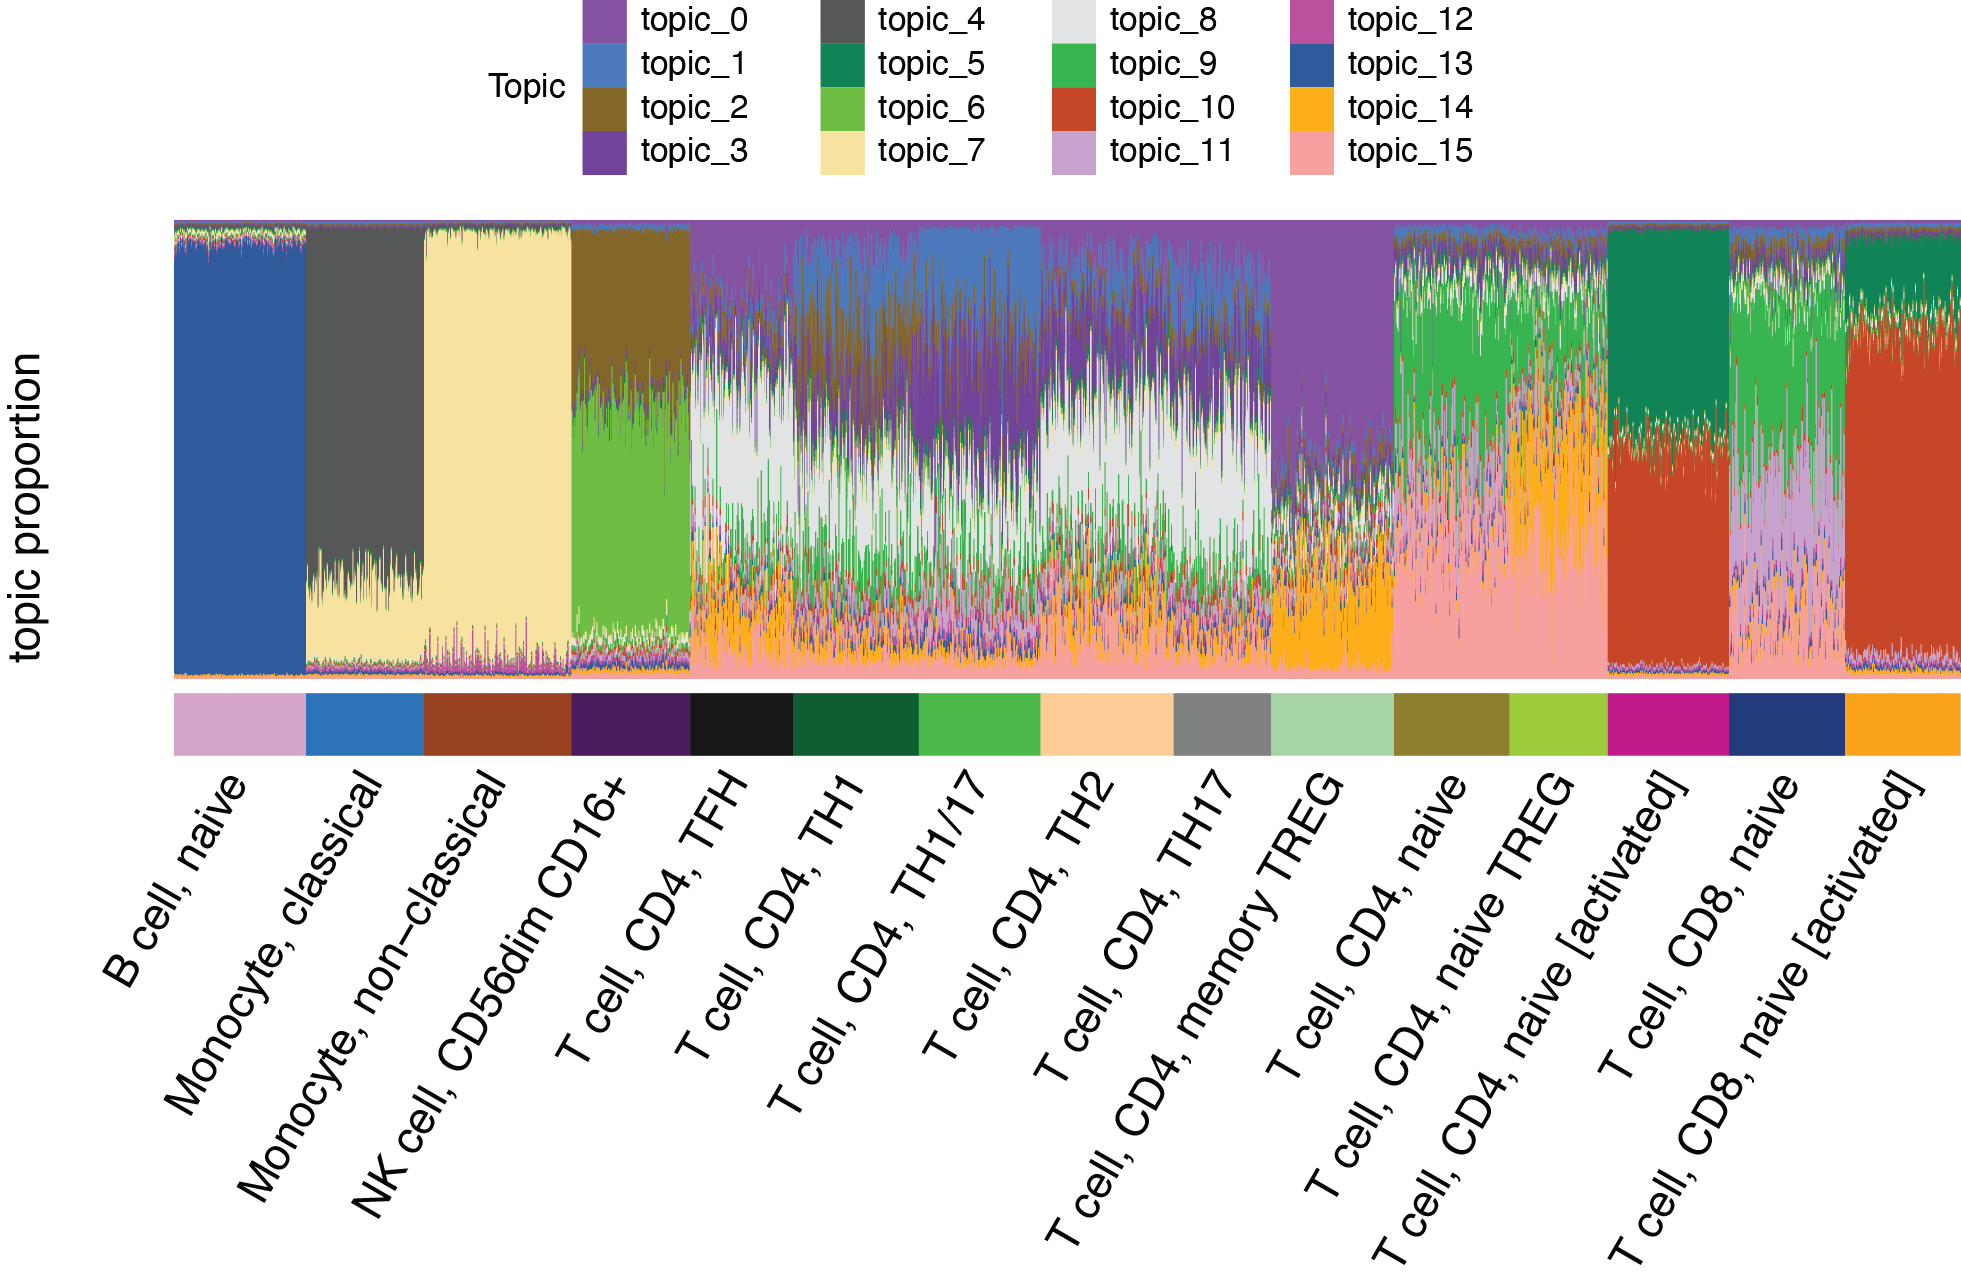
\includegraphics[width=\textwidth]{Figures/structure_plot.png}
    \caption{\textbf{Topic proportions of simulated immune cell gene expression shows distinct latent profiles between cell types} Structure plot of estimated topic proportion $\theta$ values for each cell in the simulated data set. Cells are annotated below by simulated cell type.}
    \label{fig:struct_plt}
\end{figure}

\begin{figure}
    \centering
    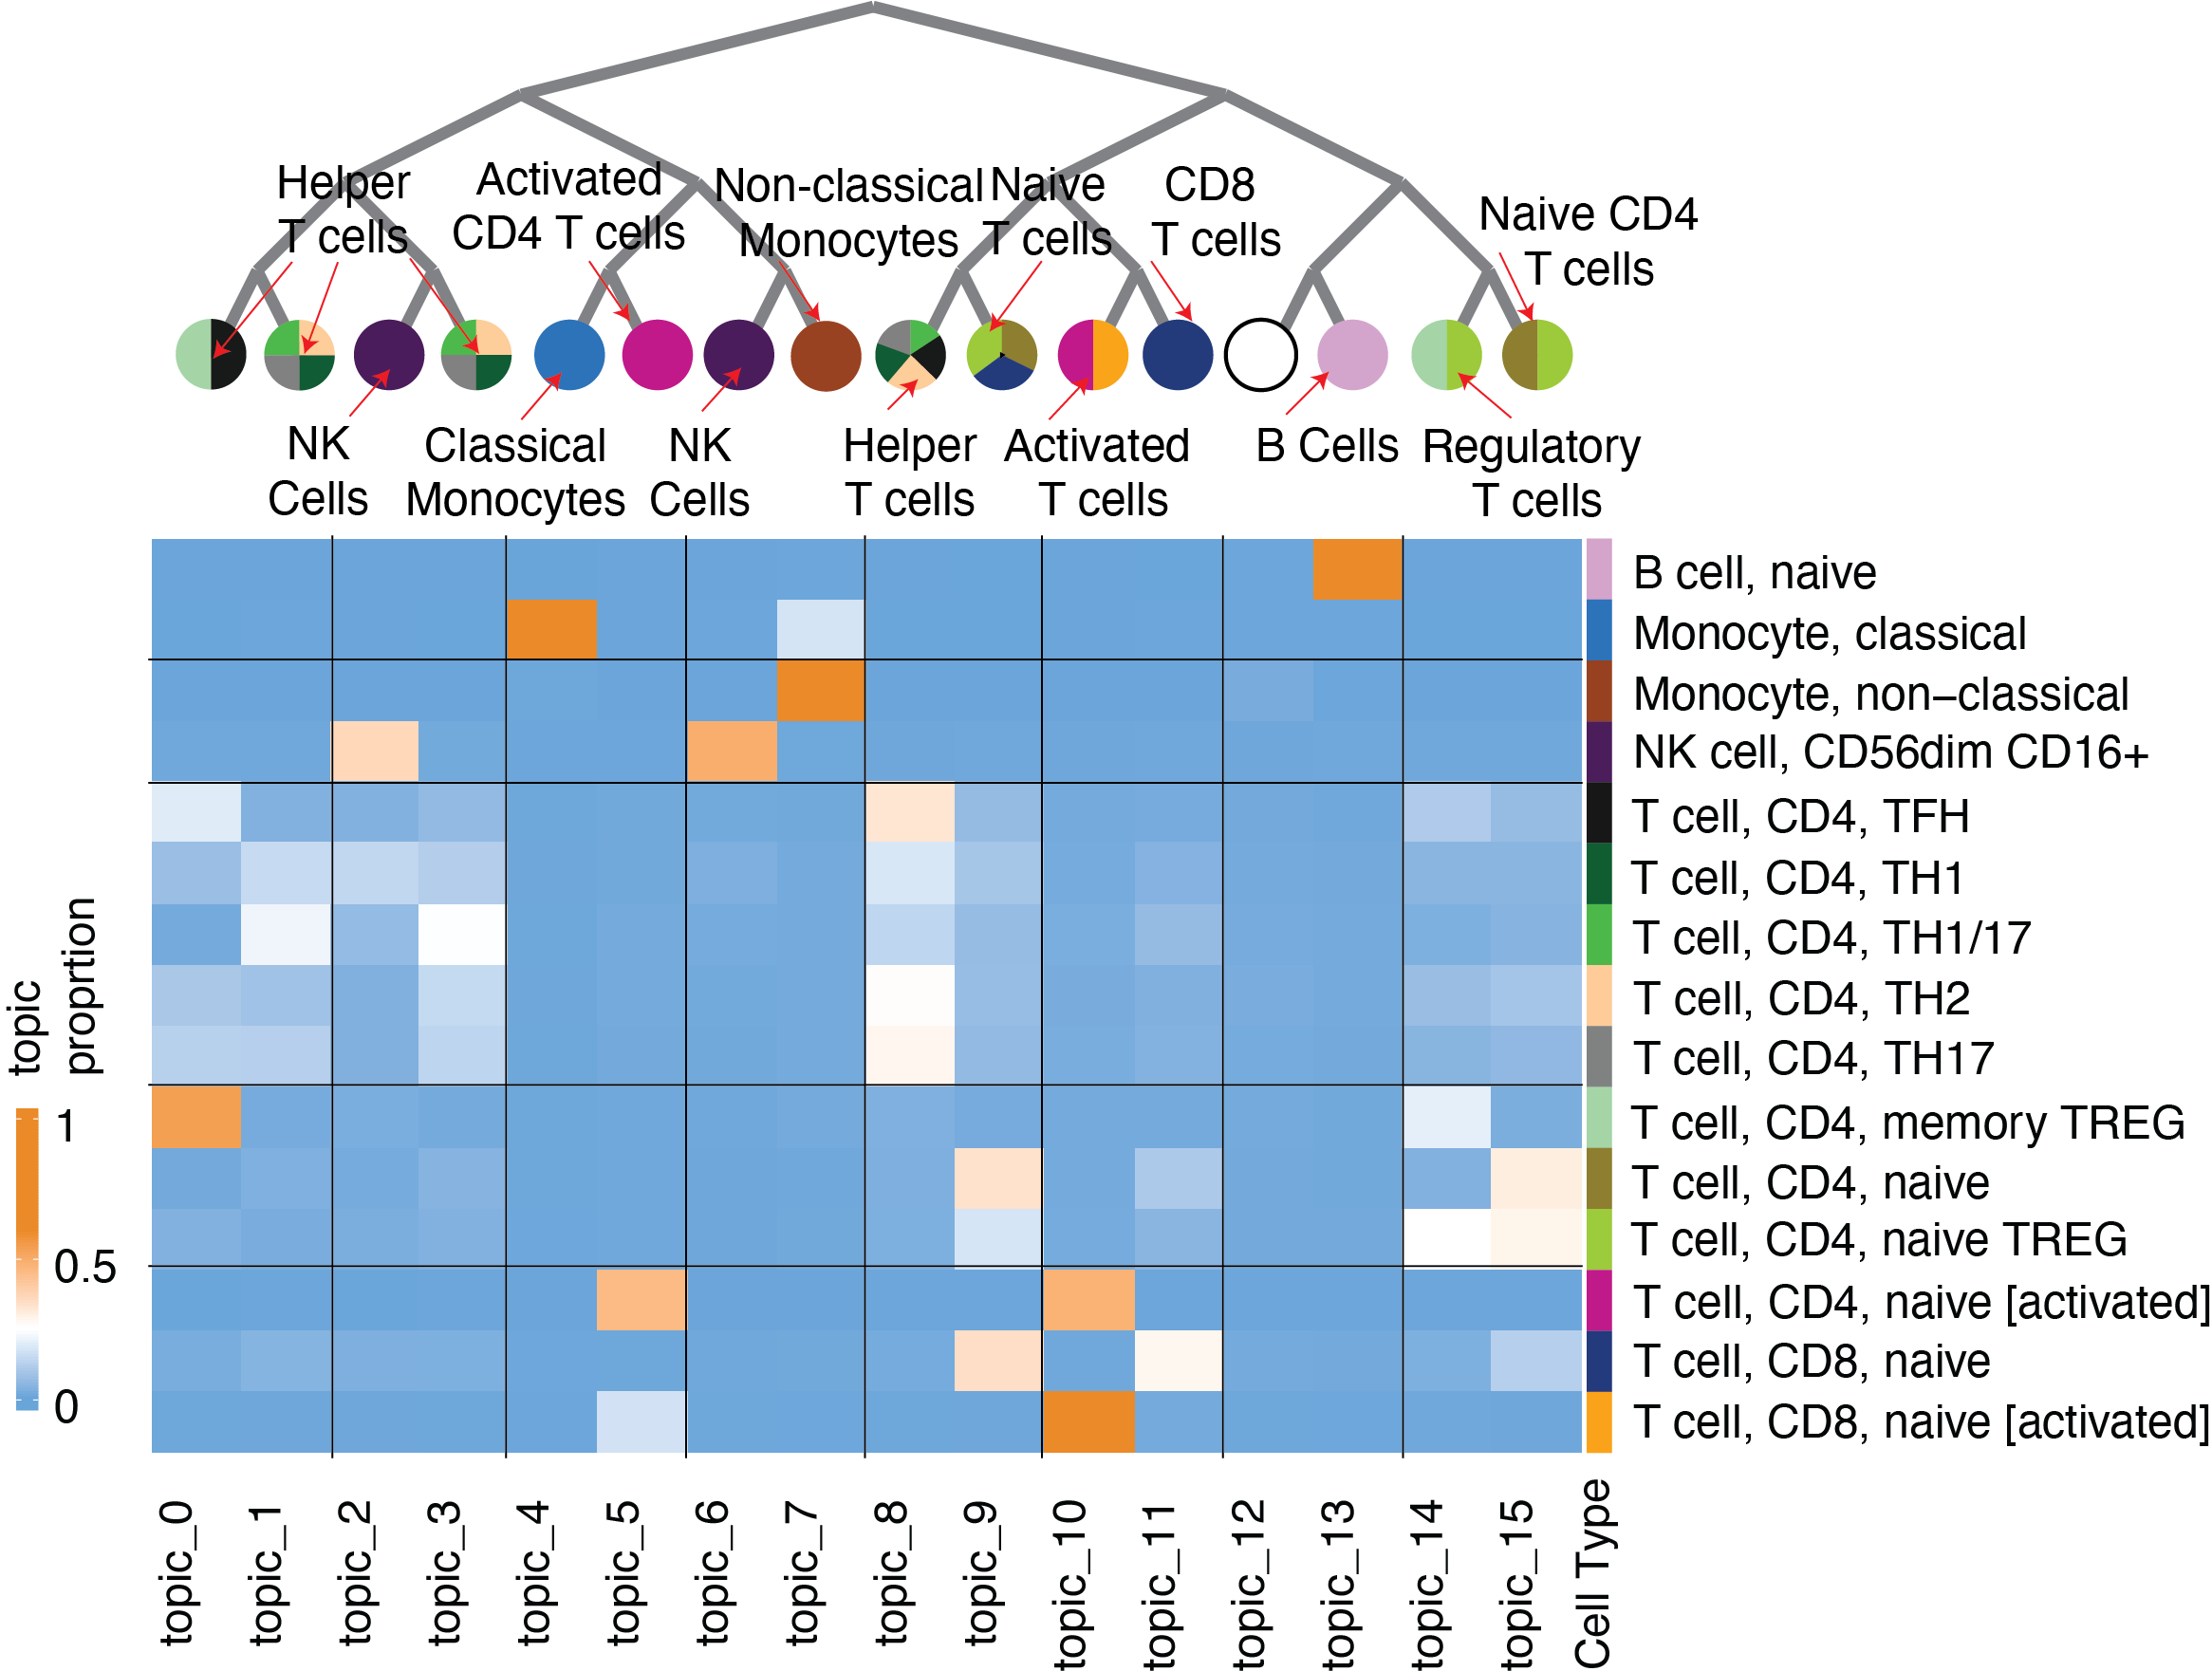
\includegraphics[width=\textwidth]{Figures/hier_hm.png}
    \caption{\textbf{Latent topic profiles can be used to reconstruct tree-structured relationships between cell subsets} The top panel shows the reconstructed tree structure from average latent topic profiles calculated for each cell subset. Below is a heatmap of the mean latent topic proportion profiles across each immune cell subset.}
    \label{fig:hier_hm}
\end{figure}

The LaRCH model was trained on a simulated immune cell scRNA-seq dataset with simulation parameters:
\begin{itemize}
    \item Number of cells $N = 2000$
    \item Noise proportion $\rho = 0.5$
    \item Read depth $R = 2500$
\end{itemize} 
and model parameters:
\begin{itemize}
    \item tree depth $D = 5$
    \item prior inclusion probability $\pi_0 = 0.1$
    \item prior normal variance $\tau_0 = 1$
    \item batch size $|s| = 128$ for $s \in [S]$
    \item learning rate $lr = 0.01$
    \item local KL weight term $kl\_weight = 1.0$
    \item beta KL weight term $kl\_weight\_beta = 1.0$
\end{itemize}

The model is able to recover the simulated cell types and represent each cell subset with a unique topic profile (Fig. \ref{fig:struct_plt}). Biologically similar cell types share topics. This is seen most prominantly amongst helper CD4+ T cell subsets which contain mixtures of topic 1, 3, and 8 (Fig. \ref{fig:hier_hm}). This suggests that the these cell subsets share overlapping expression features. The minor differences in proportions of each topic for each cell subset demonstrates that each helper T cell subset expresses the genetic features captured by each topic to varying levels. Topic 14 is highly represented in regulatory CD4+ T cell subsets, suggesting a regulatory signature being captured in the leaf node within this topic. Similarly, topic 15 is seen in naïve CD4+ T cells, possibly capturing a naïve signature.

Using the topic average latent topic representations of cell subsets, the underlying tree structure is reconstructed qualitatively (Fig. \ref{fig:hier_hm}). Topics with high representation of particular subsets are labeled as a marker topic for said subset. The reconstructed cell hierarchy shares some noticeable similarities to the lineage tree representation of immune cell subsets (Fig. \ref{fig:immune-cells}). 

The latter half of the tree representation contains only cells within the adaptive immune system. Monocytes, which branch from the other subsets at the earliest point in the differentiation process, are solely contained within topics 4 and 7 which share 3 nodes along their paths. Activated CD4+ T cells share a path with classical monocytes, suggesting some activation features captured in their shared nodes. 

Similarly, NK cells, which are involved in both innate and adaptive immune function, are represented in topic 7, sharing a node path with non-classical monocytes and it is likely that innate immune response gene signatures are captured within their shared paths, especially in nodes 4 and 10 which are not shared by any other subsets. NK cells are also represented by topic 2 which shares a node path with topic 3 which represents a number of helper T cell subsets. The shared nodes between these topics (nodes 1, 3, 8) likely contain gene embeddings related to adaptive immune response.

Topics 8 through 11 solely represent T cell subsets, capturing overlapping T lymphocyte gene expression patterns. More distinct cell types are contained within unique branches of the tree, such as B cells which are the only cell type represented in the branch containing topics 12 and 13.

Topic 14 captures features of regulatory T cell subsets which topic 15 captures those of naïve CD4+ T cells. This suggests that the nodes that constitute the shared path between these two topics (nodes 0, 2, 6, and 14) contain embeddings of genes related to CD4+ T cell function that are shared between all these T cell subsets, while node 29, the leaf node of topic 14 contains gene embeddings related to regulatory function and node 30, the leaf node of topic 15 is related to naïve expression profiles. 



\subsection{Using Latent Features in Place of Other Dimensionality Reduction Techniques for Downstream Analysis}
\begin{figure}
    \centering
    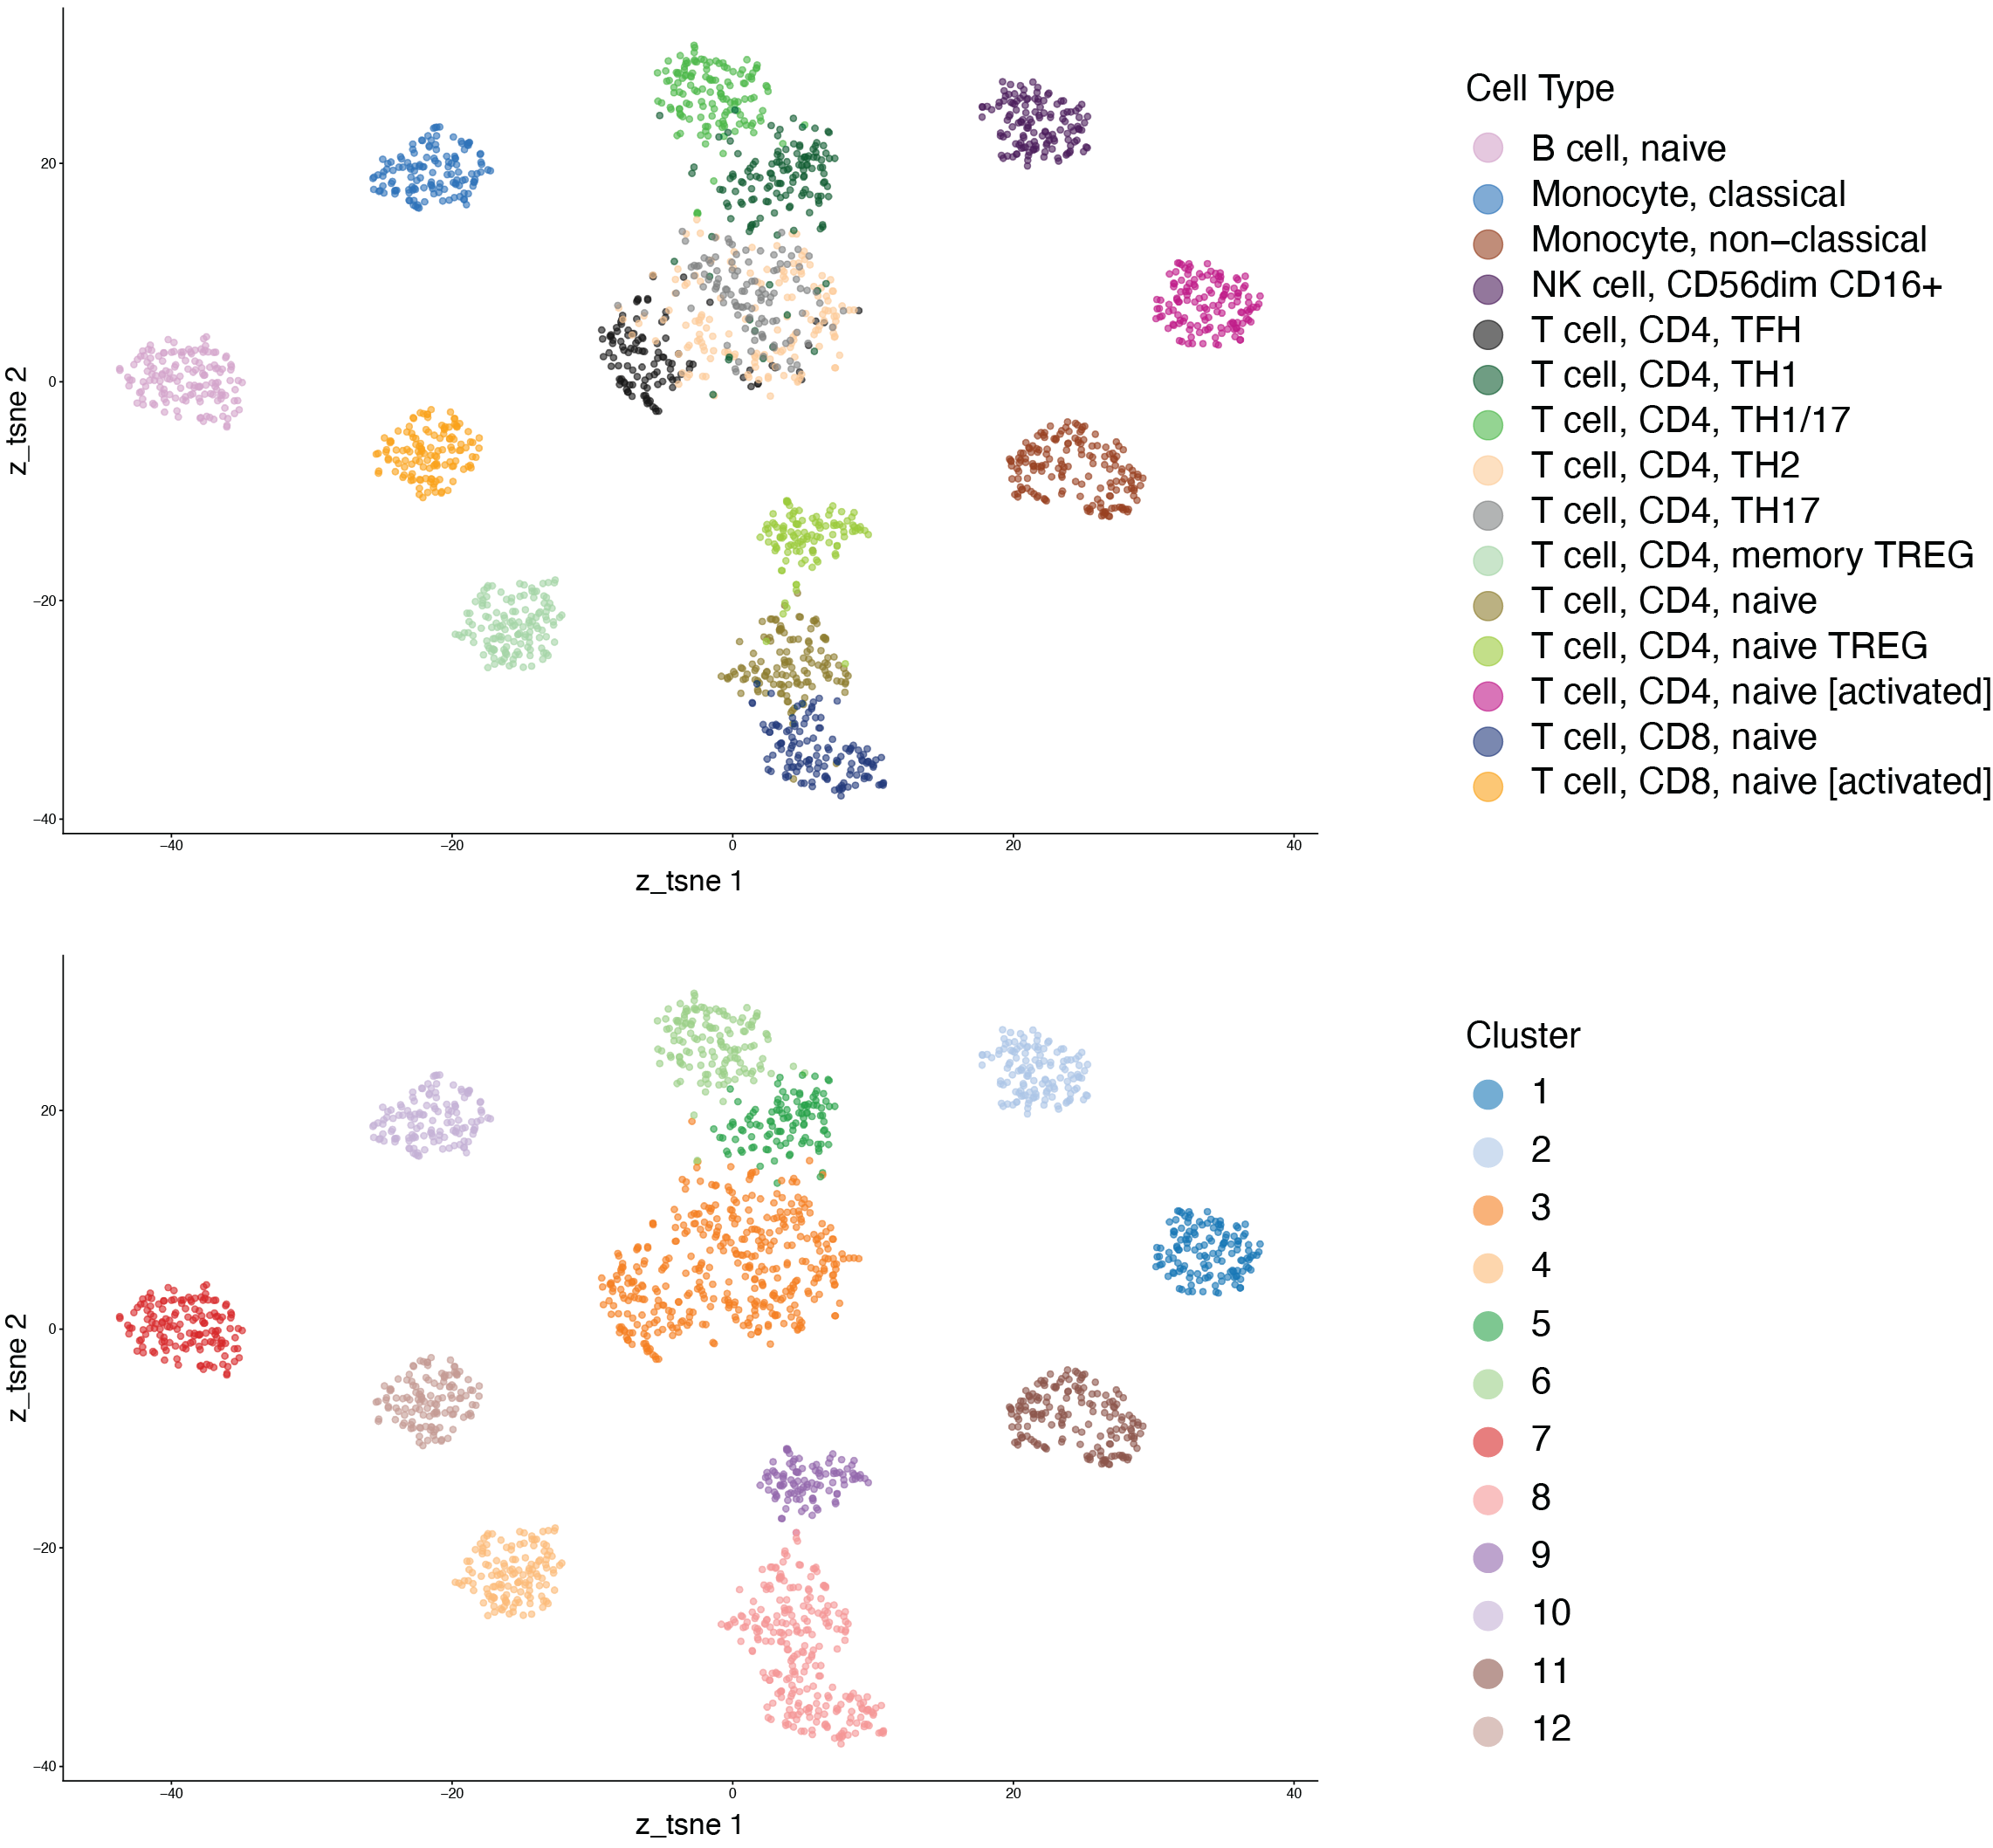
\includegraphics[width=\textwidth]{Figures/cluster_tsne.png}
    \caption{\textbf{Louvain lustering on latent topic space recovers groups of cells corresponding to their simulated cell type} The top panel shows the simulated cells in tSNE space coloured by original simulated cell type. The bottom panel shows the clusters generated using louvain clustering on the latent topic representation of cells. For visualization, tSNE dimensions were generated from the latent topic space.}
    \label{fig:sim_clusters}
\end{figure}

To test the efficacy of the LaRCH model and its ability to perform cell type deconvolution from single-cell gene expression data, clustering was performed using the latent topic features estimated from simulated data. 

The Louvain method of community detection \cite{louvain} was used to extract cell type clusters from a K-nearest neighbour graph ($k = 10$ was used) constructed using the latent topic features to calculate distance between data points. In general, the resulting cell clusters separate the various simulated cell types, missing only some granularity between closely related cell types (Fig. \ref{fig:sim_clusters}). In this case, the clustering done is unable to distinguish between certain subsets of T cells. The helper T cell subsets of T follicular helpers, Th17s, and Th2s are all contained within cluster 3 from figure \ref{fig:sim_clusters}, it is seen that these cells lie closely in the t-distributed stochastic neighbor embedding (tSNE) reduced dimension space, showing that the simulated transcriptional profiles of these cell are very similar. Additionally, cluster 8 contains the naïve subsets of both CD4+ and CD8+ cell types. The grouping of these cell types within the latent feature space suggests an overlap in overall gene expression profile and cellular function between cell types. Changing Louvain clustering parameters ($k = 5$) creates a more granular clustering that more accurately separates individual cell types, but this also runs the risk of over-clustering. 

\begin{figure}
    \centering
    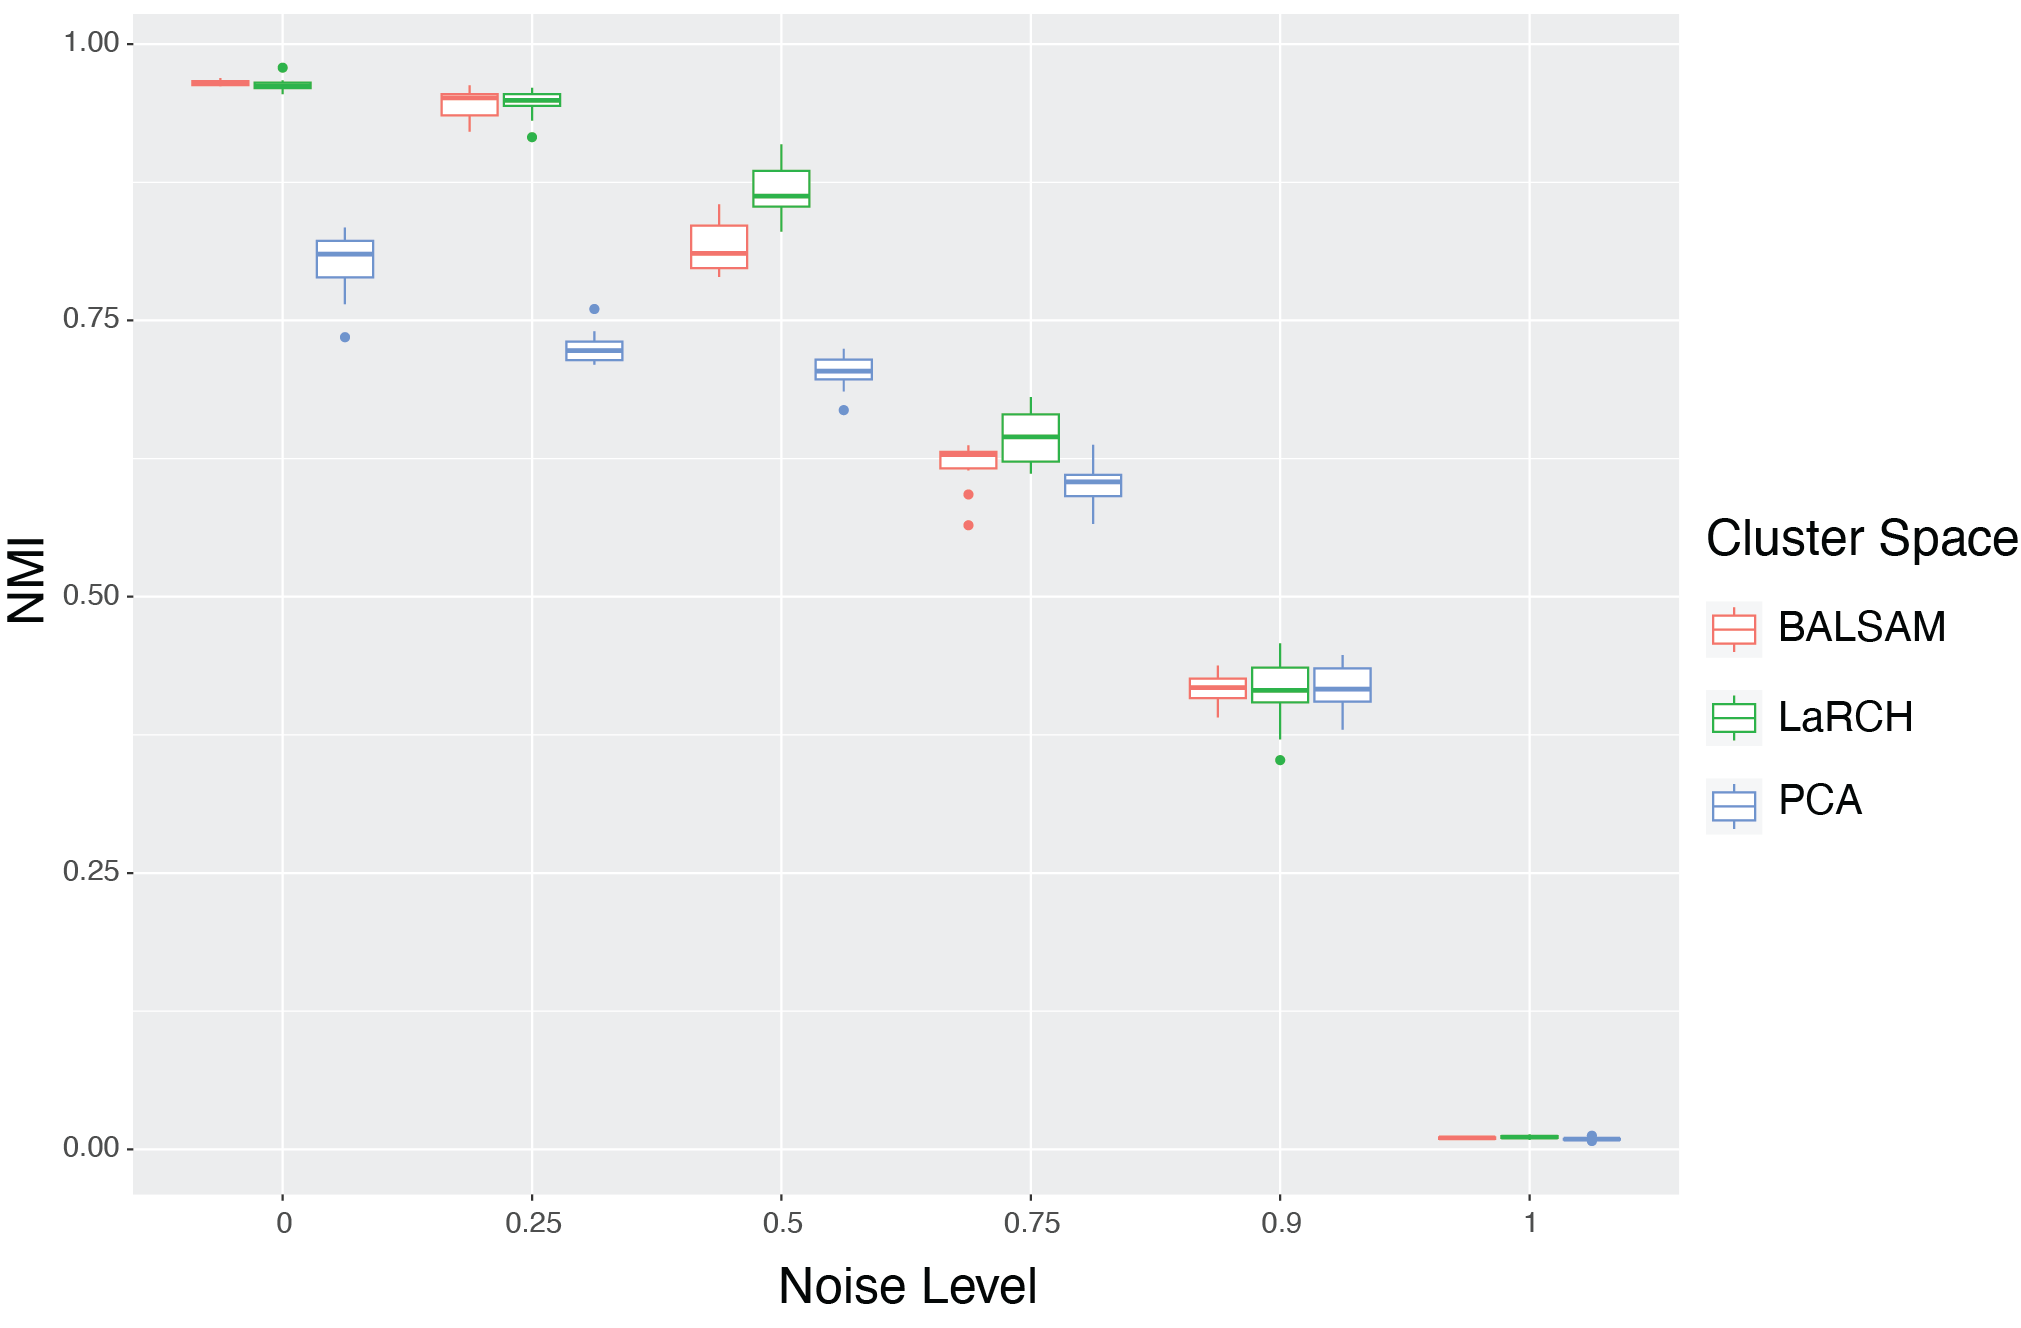
\includegraphics[width=\textwidth]{Figures/nmi_comp.png}
    \caption{\textbf{Using the LaRCH latent space for clustering consistently outperforms clustering on PCA and flat latent topic space} NMI calculated from clustering results from each dimensionality reduction technique and the original simulated cell types across various noise levels. At each noise level, 10 datasets were simulated with different starting seeds.}
    \label{fig:nmi}
\end{figure}

Clustering results from latent topic features as the clustering space were compared to clusters obtained from the first 50 PCs as well as BALSAM \cite{ZHANG2023100388} with 16 latent topics, the same number of latent topics as a LaRCH model with depth $D = 5$. BALSAM is a comparable ETM that utilizes the same encoder-decoder scheme as LaRCH without the underlying tree structure. At each noise level ($\rho =$ 0, 0.25, 0.5, 0.75, 0.9, 1), 10 datasets were simulated with different starting seeds. The Louvain method of community detection \cite{louvain} was then used to detect clusters from the K-nearest neighbour graphs ($k = 10$ was used) constructed from each reduced dimension space. The normalized mutual information (NMI) was calculated from each clustering result and original simulated cell types to compare clustering accuracy (Fig. \ref{fig:nmi}). 

At all noise proportions, clustering from the LaRCH latent feature space outperforms PCA clusters. At low noise proportions, BALSAM and LaRCH are comparable in NMI while at mid-level noise proportions ($rho = 0.5$ and $\rho = 0.75$), LaRCH performs slightly better than BALSAM, showing that the underlying tree-structure provides additional insight on cell type features to the latent topics that are not captures in a flat model. At $rho = 0.9$, where the simluated data is primarily noise and no longer realistic in its representation of a real scRNA-seq dataset, the NMI drops below 0.5 and all clustering methods struggle. 



\chapter[Modeling Cellular Hierarchies\dots]{Modeling Cellular Hierarchies in a Real scRNA-seq Dataset}
\label{cha:sle}
As a practical application of the LaRCH model, the model is trained on a real single-cell RNA-seq dataset used to study the cell-type specific molecular and genetic associations of SLE \cite{sledata}. In this section, details of the scRNA-seq data are described and the resulting model trained on the dataset is used to explore various aspects of the disease pathogenesis of SLE.

\section{Single-cell RNA-seq data from a large SLE dataset}

The scRNA-seq dataset used to train the model is from a 2022 paper from Perez \textit{et al}. \cite{sledata}. This dataset consists of single-cell transcriptome data of 1.2 million PBMCS from 99 healthy control individuals and 162 individuals with SLE. 

\subsection{Dataset Details}

PBMC samples used in this analysis were collection from SLE cases in the California Lupus Epidemiological Study (CLUES) cohort. Matched healthy control samples were collected from the UCSF Rheumatology Clinic and the Immune Variaton Project (ImmVar) \cite{sledata}.

Single-cell gene expression profiles from pooled antibody-stained and unstained PBMCs was generated using 10x Genomics' Chromium Single Cell 3' V2 chemistry and processed with the 10x Cell Ranger pipeline. Filtered scRNA-seq read count data was obtained directly from accession number \href{https://www.ncbi.nlm.nih.gov/geo/query/acc.cgi}{GSE174188} in the Gene Expression Omnibus (GEO). Additionally, patient metadata, cell type annotation, and UMAP projections from the original study were used for the data analysis in this chapter.

\newpage 
\section{Deconvolution of Immune Cell Subtypes}

\begin{figure}
    \centering
    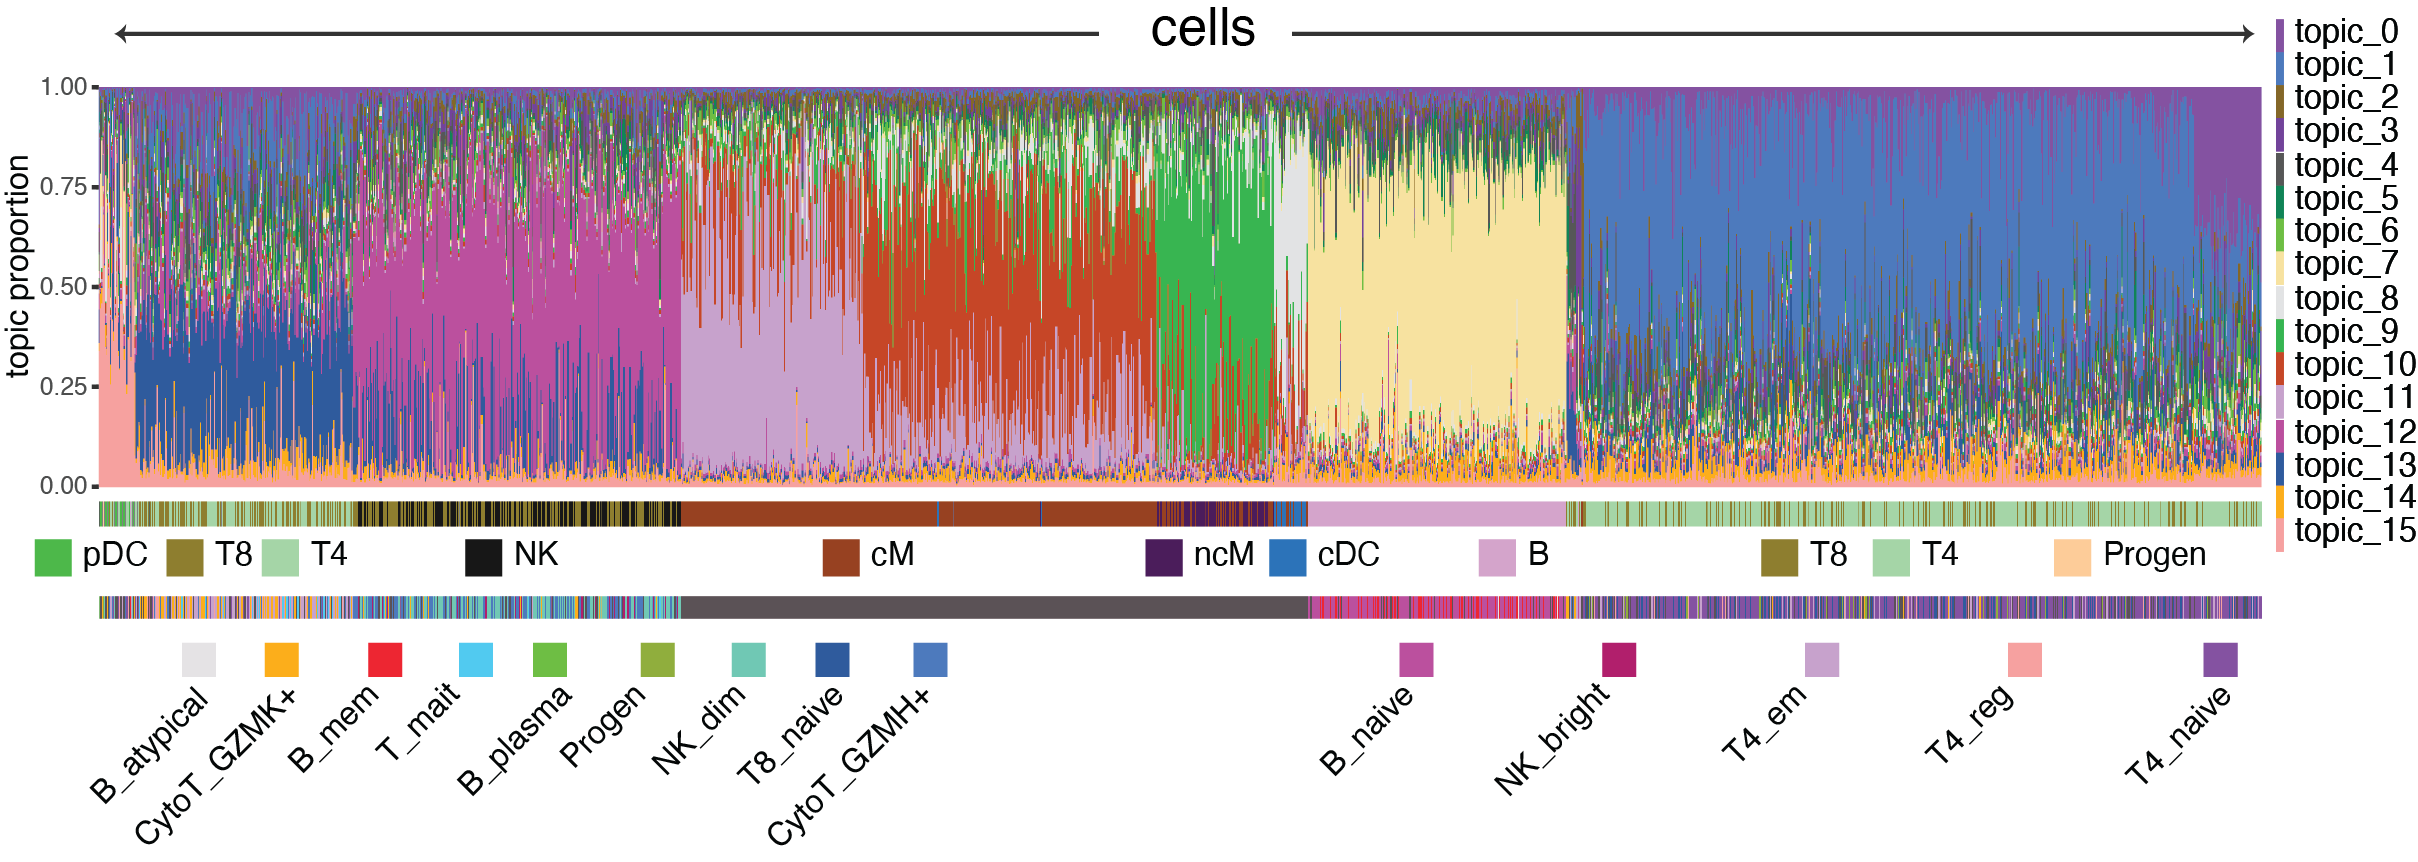
\includegraphics[width=\textwidth]{Figures/struct_plt.png}
    \caption{\textbf{Distinct topic proportions of PBMCs in a scRNA-seq dataset of SLE and healthy individuals correspond to cell type labels} Structure plot of estimated $\theta$ values for a subsample of 10,000 cells in the data set. Cells are annotated below by labelled cell types obtained from Perez \textit{et al.} \cite{sledata}}
    \label{fig:sle_struct}
\end{figure}

Estimated topic proportion profiles show distinct groups of cells within the latent space that align closely with the cell types determined in the original Perez \textit{et al.} paper \cite{sledata} (Fig.\ref{fig:sle_struct}). The topic representation of cells is able to pick up more granularity that potentially describes further distinct cell types, namely in the cells labelled as 'classical monocytes' where there are two distinct groups in the topic space primarily represented by either topic 10 or topic 11, suggesting classical monocyte-labeled subsets could be composed of subsets with differing cell function. 

\begin{figure}
    \centering
    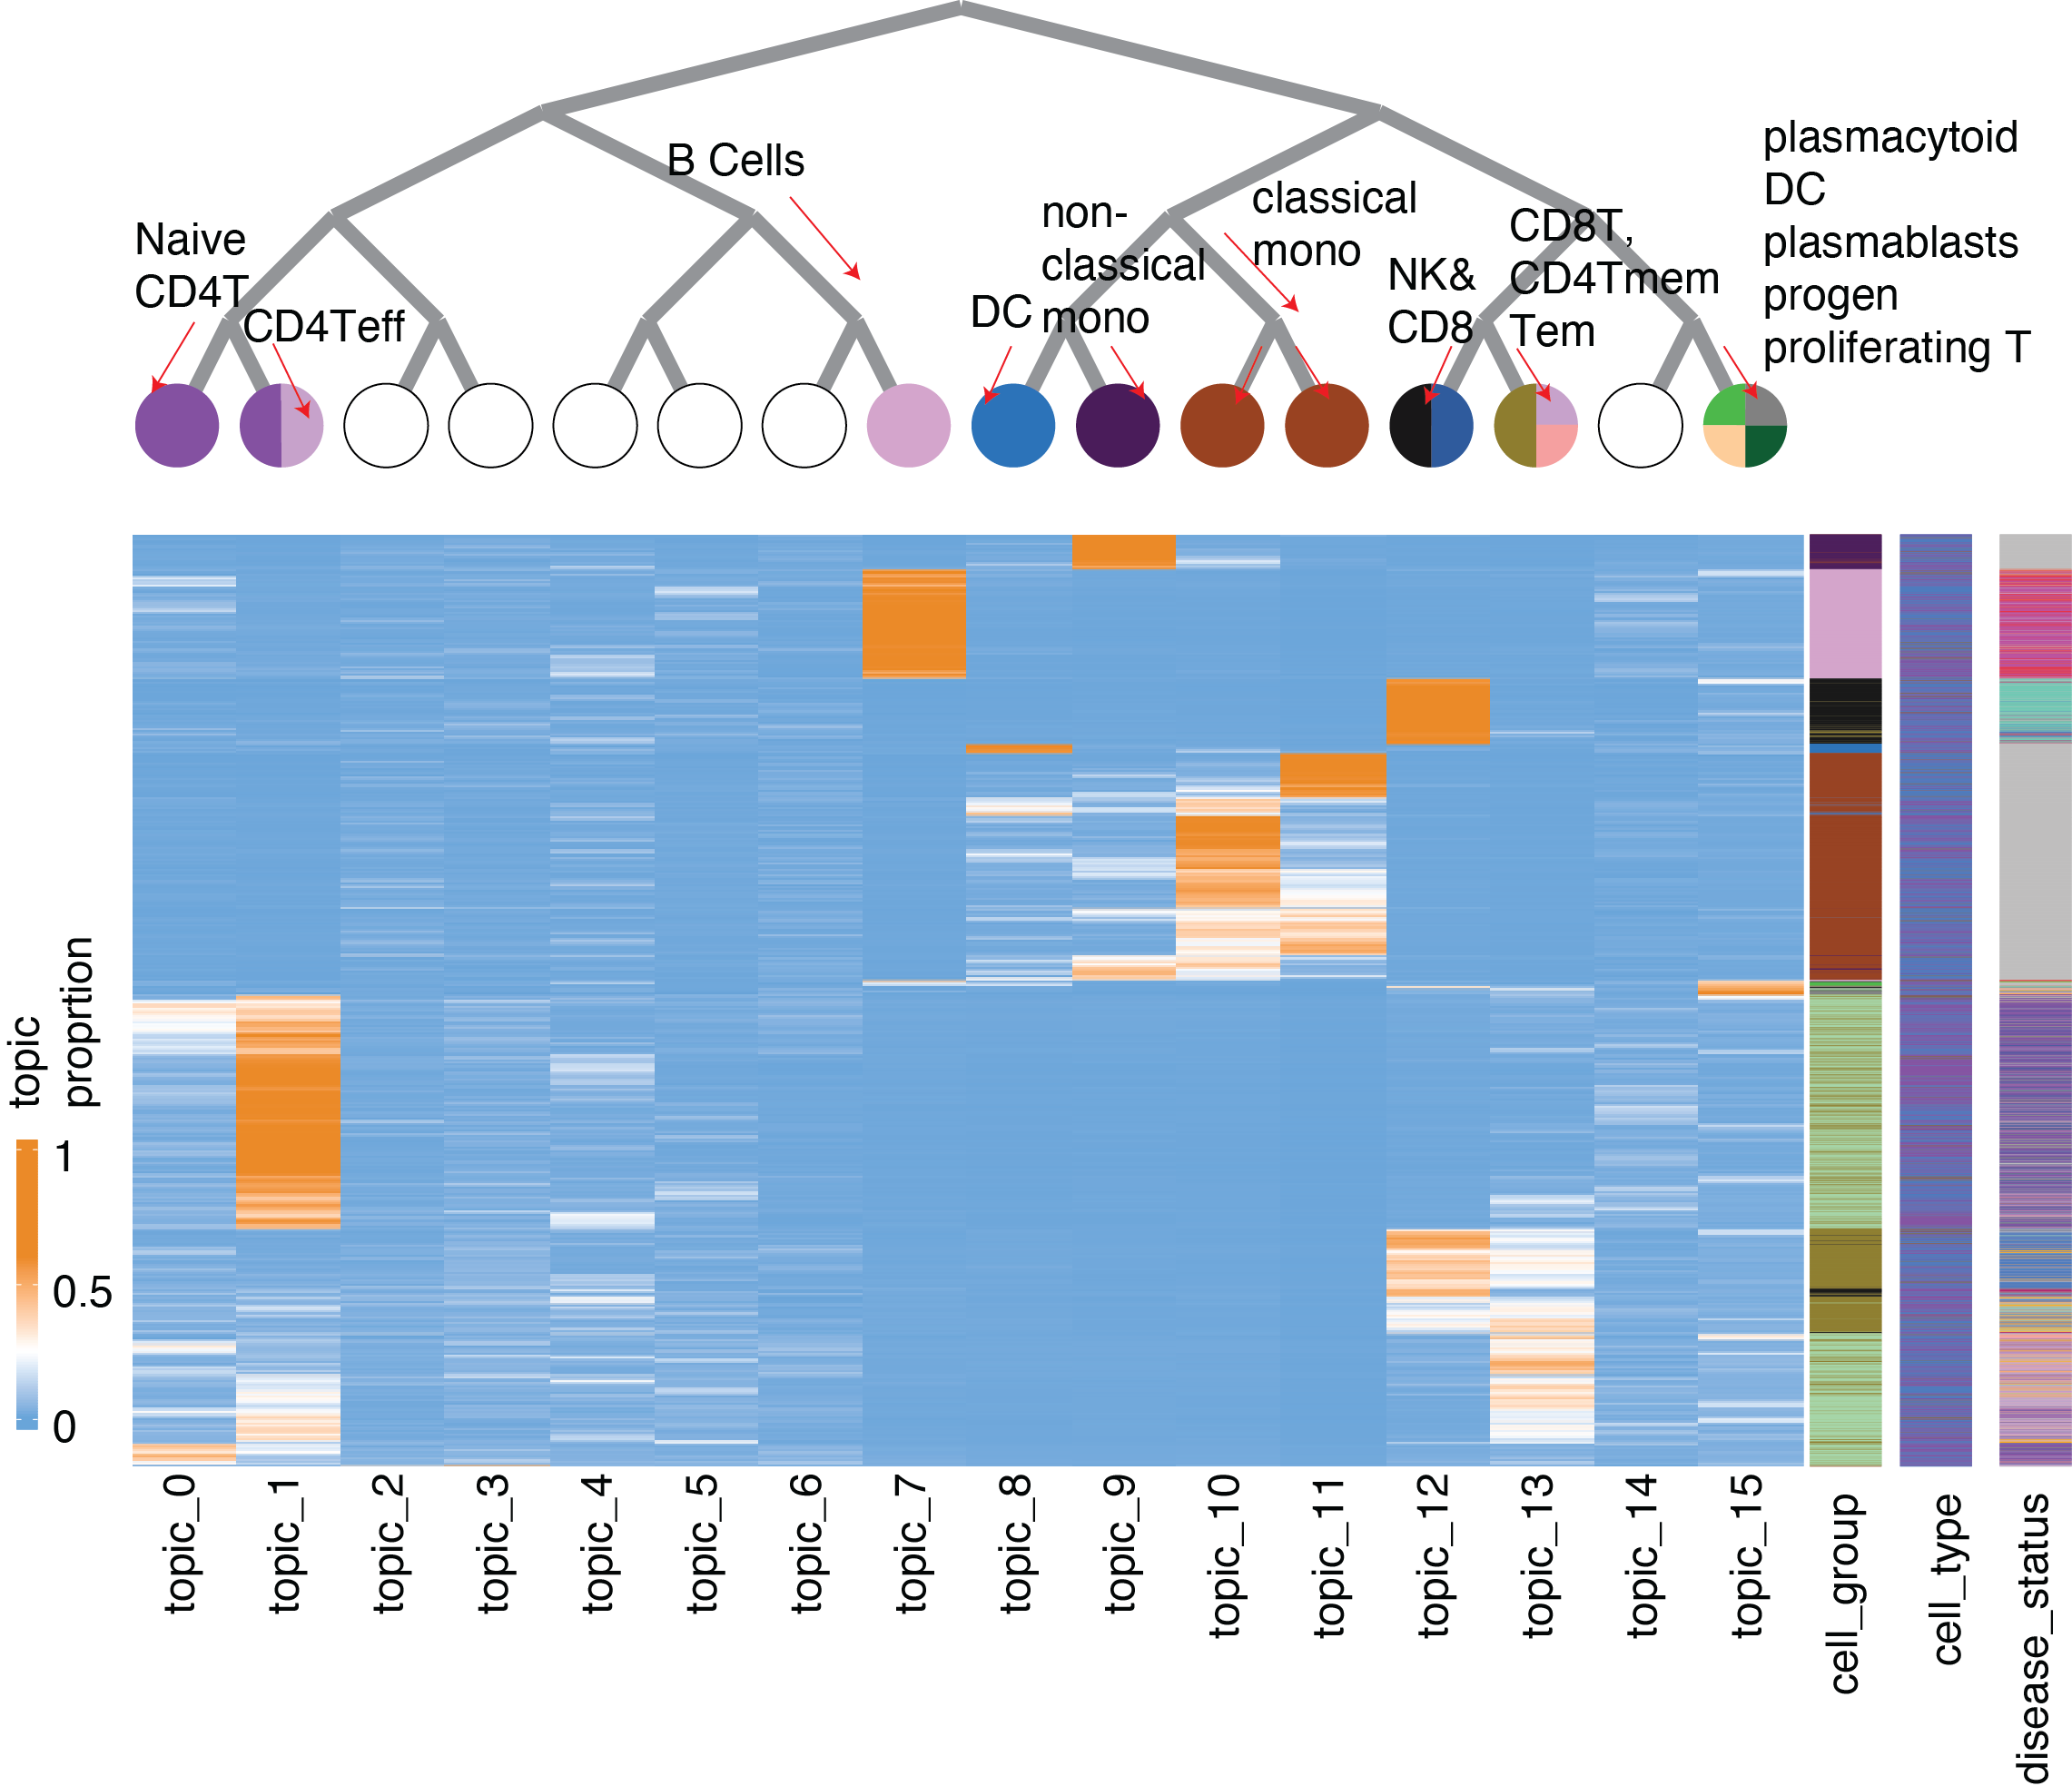
\includegraphics[width=\textwidth]{Figures/hier_tree.png}
    \caption{\textbf{Tree-structure relationships between cell types are reconstructed using latent topic profiles of a real scRNA-seq dataset} The top panel shows the reconstructed tree structure based on average latent topic profile representations of cell types. Below is a heatmap of the latent topic proportion profiles across a subset of 10,000 cells from the dataset.}
    \label{fig:sle_tree}
\end{figure}

As with the simulated data, a tree structure outlining the hierarchical relationships between cell types is qualitatively assembled using the average latent profiles of immune cell subsets. Similar to the simulated data setting, the constructed tree structure from the real data set aligns with the canonical understanding of immune cell differentiation (Fig.\ref{fig:sle_tree}). B cells lie within their own distinct branch of the tree. Myeloid cells, including monocytes and dendritic cells are contained within the tree branch with topics 8 through 11. Topic 15 captures a number of intermediate immune cell-states, including progenitor and proliferating lymphoid cells, proliferating dendritic cells, and plasmablasts. Naive CD4+ T cells are primarily represented by topic 0 and 1, while the remaining CD4+ subtypes are represented by topic 13 along with non-naive CD8+ T cells. NK cells and naive CD8+ T cells are found in topic 12. 

\subsection{Cell Clustering}
\begin{figure}
    \centering
    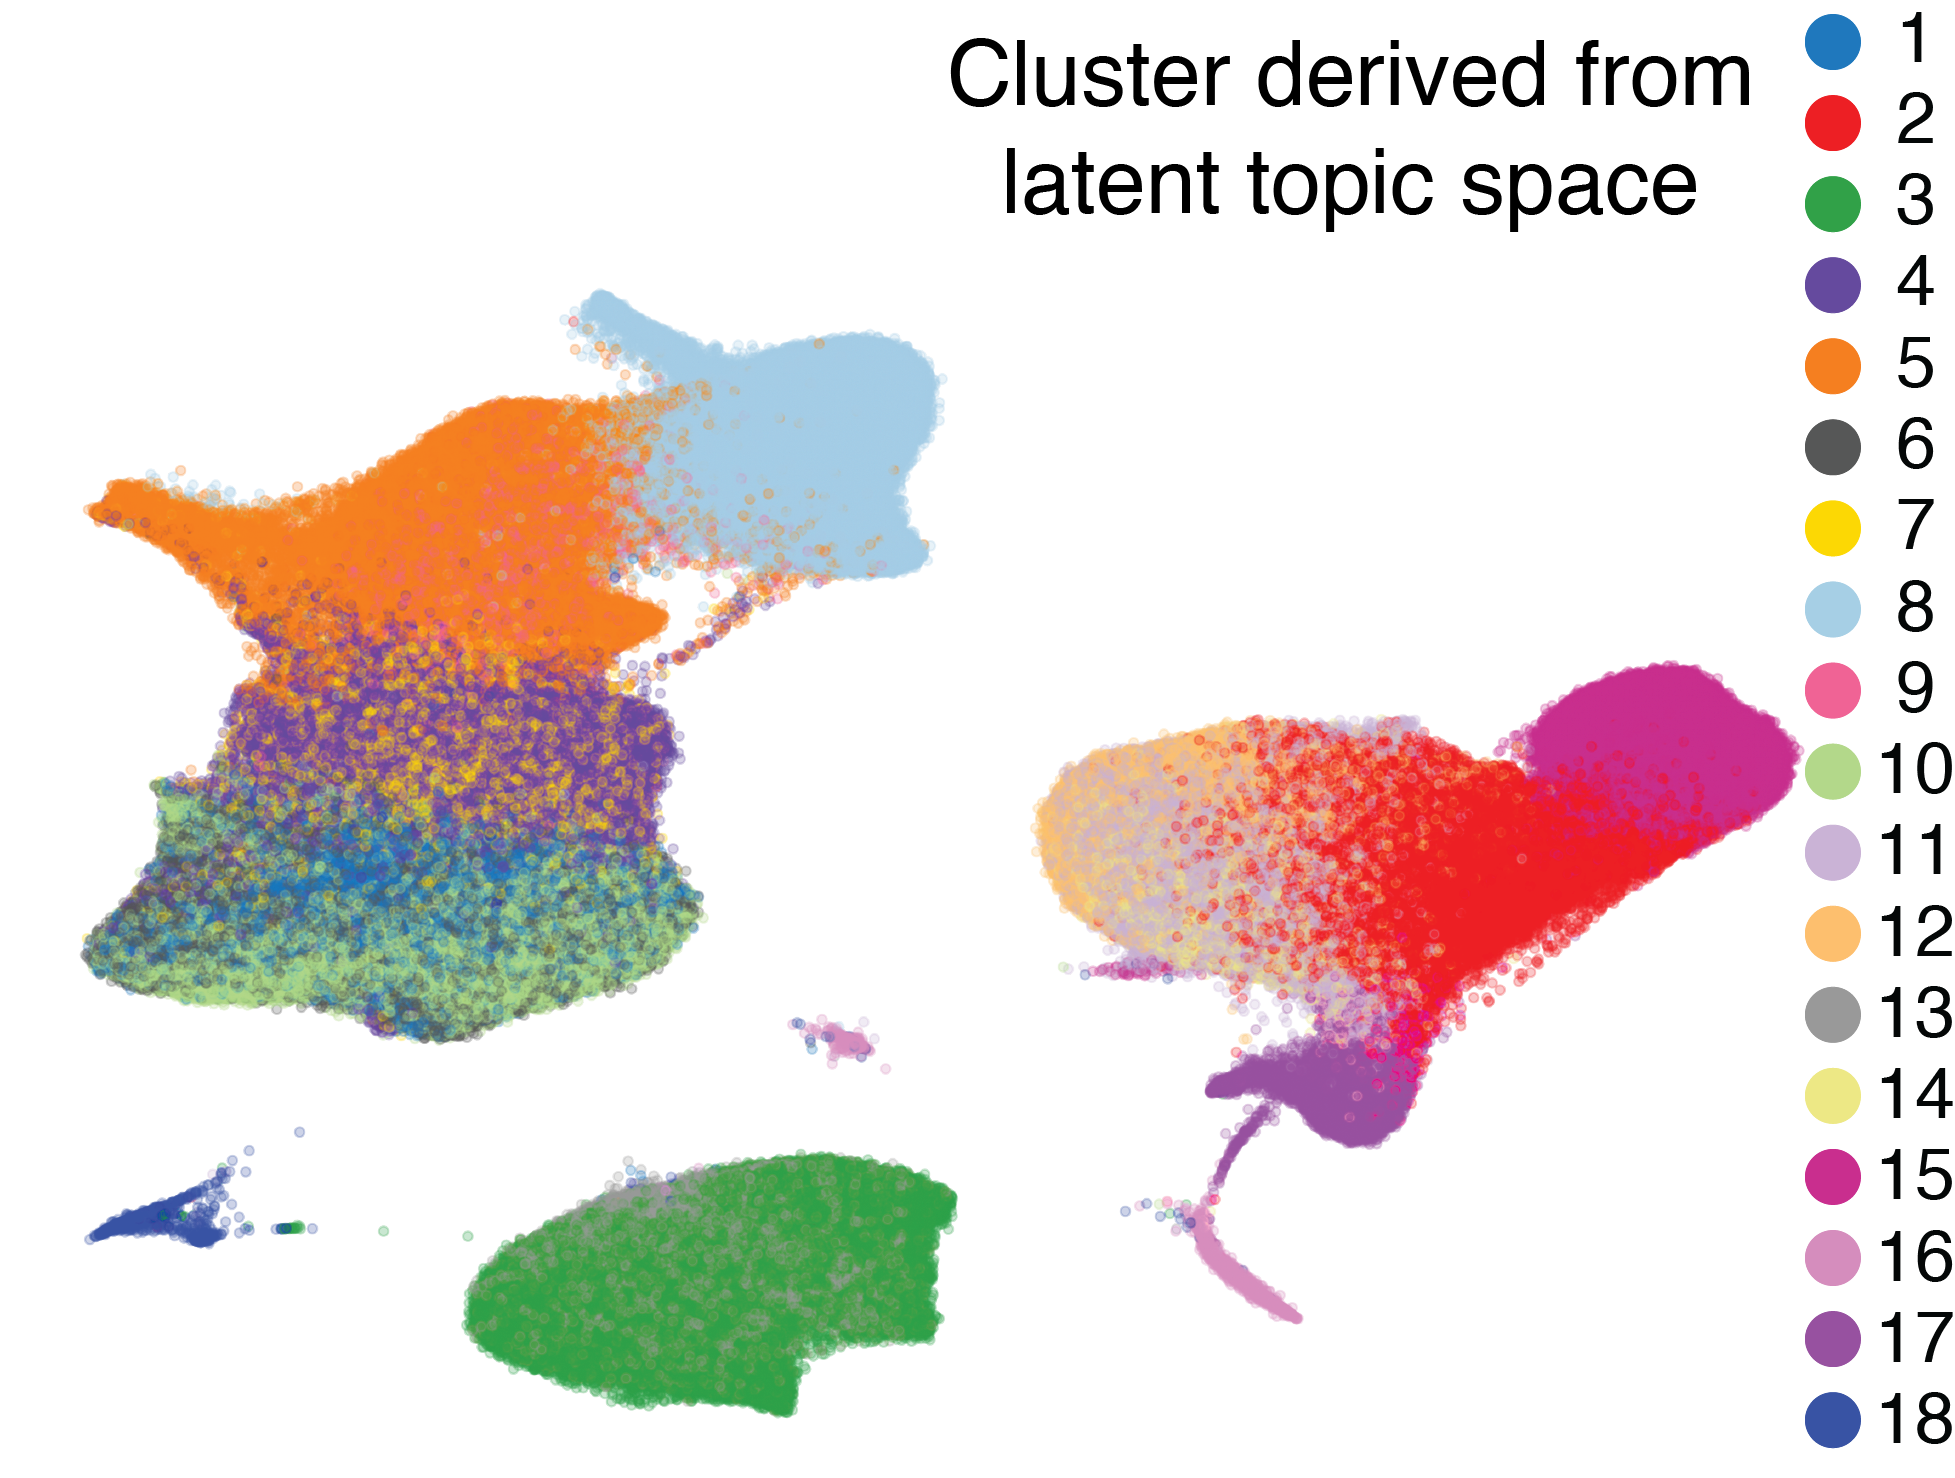
\includegraphics[width=\textwidth]{Figures/cluster_umap.png}
    \caption{\textbf{Clustering on latent topic space recovers groups of immune cells belonging to related immune subsets} UMAP projection of scRNA-seq data are coloured by Louvain clusters derived from the latent topic space. UMAP projection values obtained from the original Perez \textit{et al.} study \cite{sledata}}
    \label{fig:cluster_umap}
\end{figure}

\begin{figure}
    \centering
    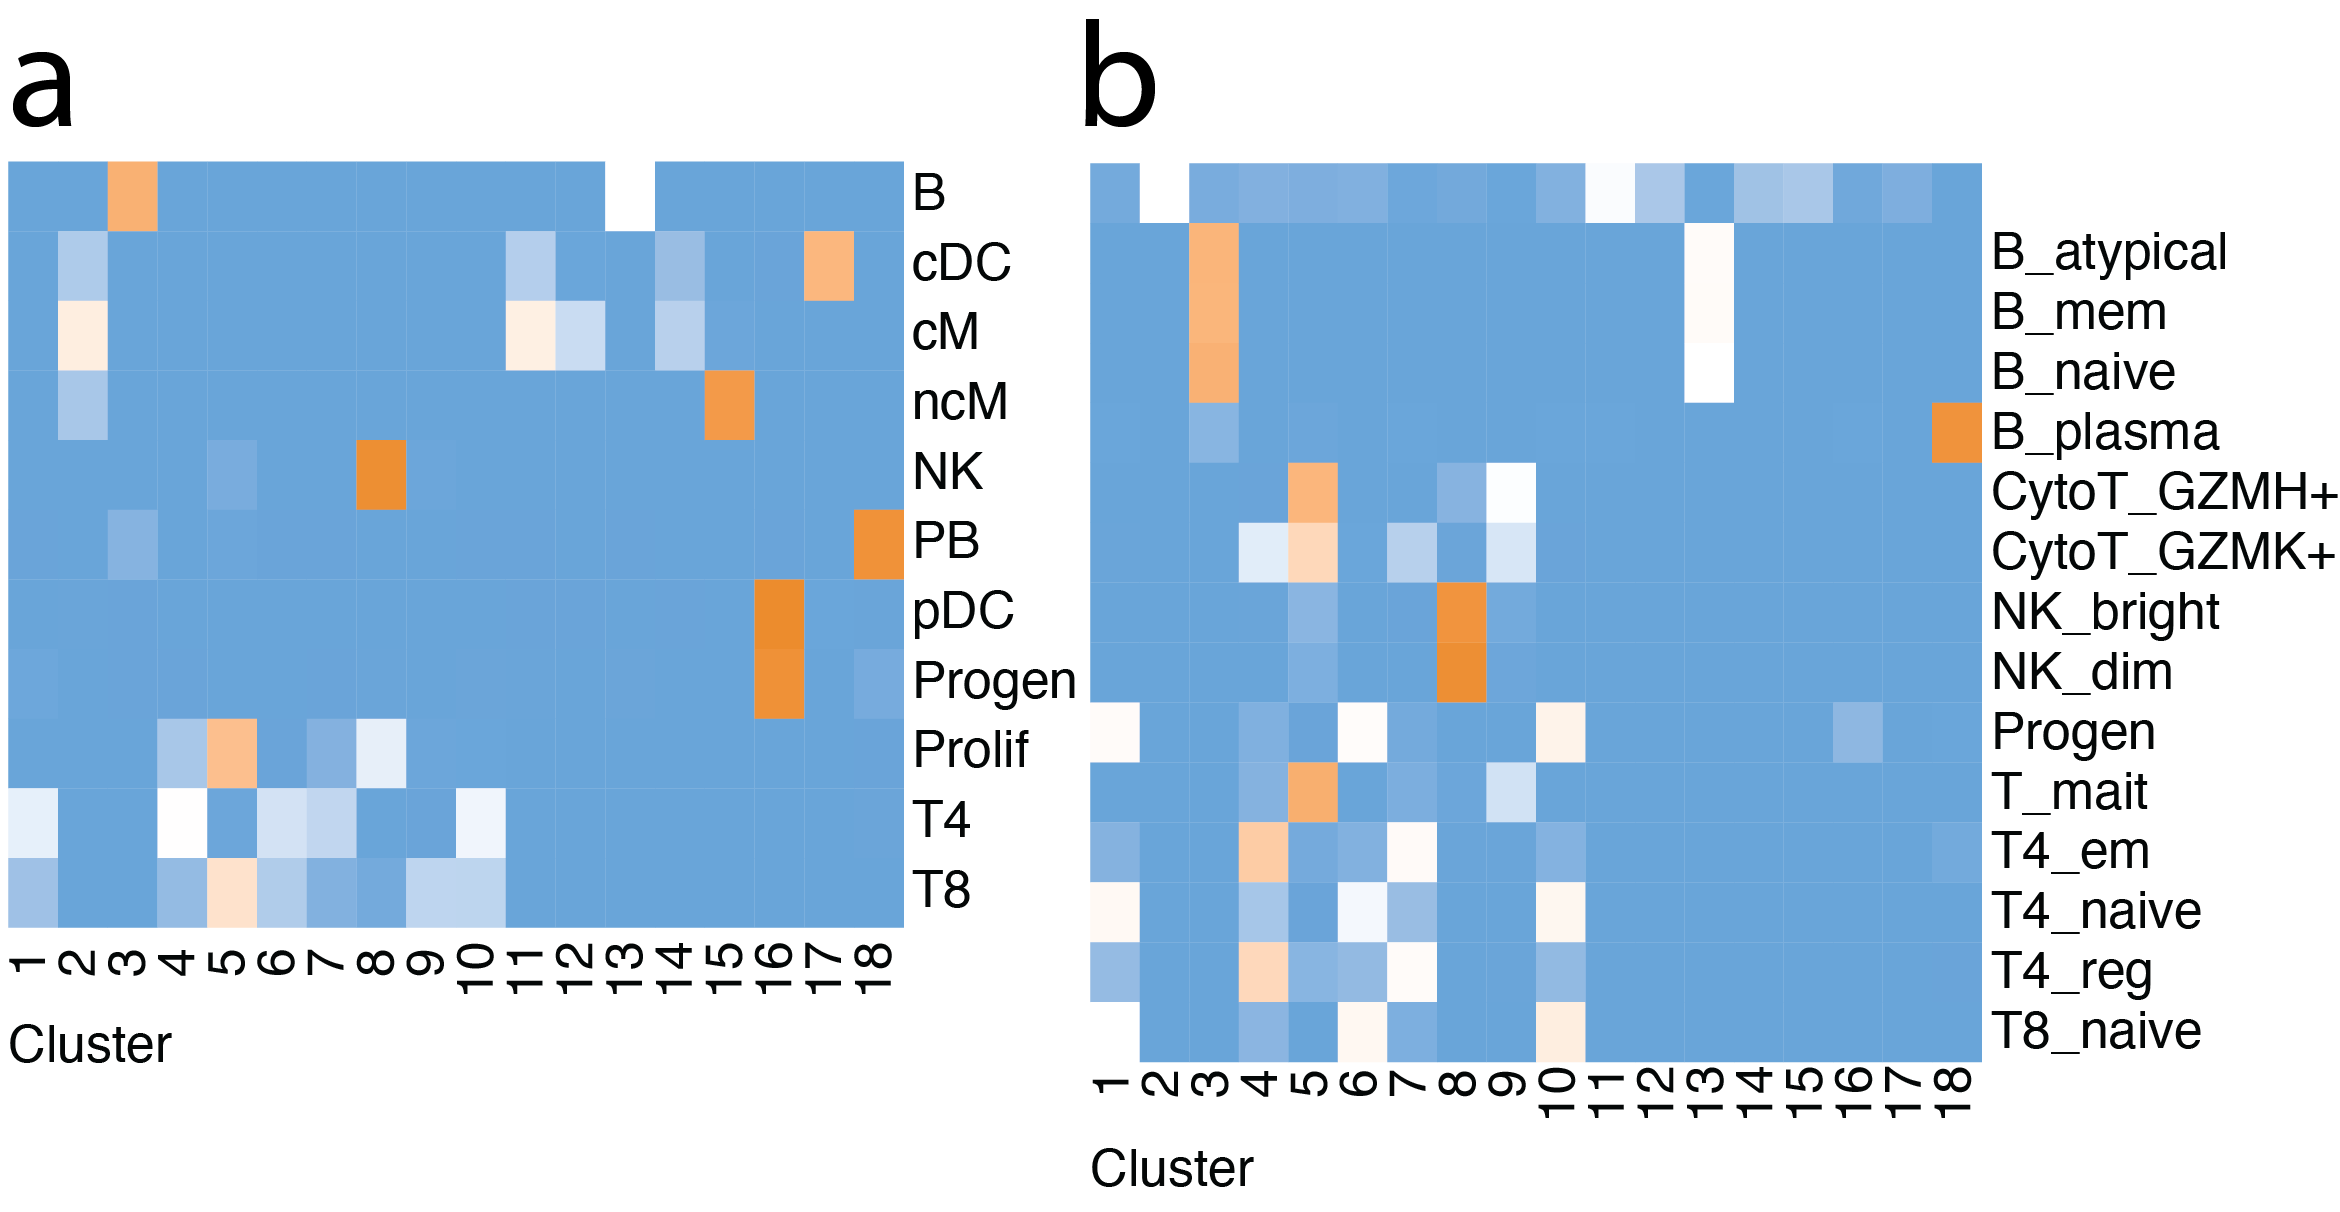
\includegraphics[width=\textwidth]{Figures/cluster_ct.png}
    \caption{\textbf{Overlap exists between latent topic clusters and original cell labels} a) Heatmap depicting the similarity matrix between louvain clusters obtained from latent topic space and cell group labels. b) Heatmap depicting  the similarity matrix between louvain clusters obtained from latent topic space and cell type labels. 
    Cell clusters are represented along the columns of the heatmap while cell labels are represented along the rows. 
    Cell group and cell types are described in \cite{sledata}. Cell groups describe more general immune cell subsets while cell types describe specific immune cell subsets.}
    \label{fig:cluster_ct}
\end{figure}

Louvain clustering \cite{louvain} using $k=30$ nearest neighbours in the latent topic space results in clustering that aligns with cell groups described by Perez \textit{et al.} \cite{sledata} (Fig.\ref{fig:cluster_umap}, \ref{fig:cluster_ct}a), but quickly loses the ability to clearly distinguish cell the more specific cell types (Fig.\ref{fig:cluster_ct}b). For this purpose, similarity is measured as the proportion of cells with a specified label contained within a cluster, mathematically this is: 
\begin{align*}
    &\text{Similarity}(\text{cell\_label}_j, \text{cluster}_k) = \\ &\frac{\sum_{i = 0}^N \mathbb{I}(\text{cell\_label}(\text{cell}_i) = \text{cell\_label}_j) * \mathbb{I}(\text{cluster}(\text{cell}_i) = \text{cluster}_k)}{\sum_{i = 0}^N \mathbb{I}(\text{cell\_label}(\text{cell}_i) = \text{cell\_label}_j)}
\end{align*} 
Where $N$ is total number of cells in the dataset and cell\_label(cell$_i$) and cluster(cell$_i$) return the assigned cell label and cluster for cell$_i$, respectively.

Since the original cell types are assigned from Louvain clustering on UMAP reduced dimensions and canonical marker gene expression, it is unclear as to which clustering method produces higher-quality immune function-relevant cluster assignments. 

\newpage
\section{Disease Dependent Differences in Expression}

\begin{figure}
    \centering
    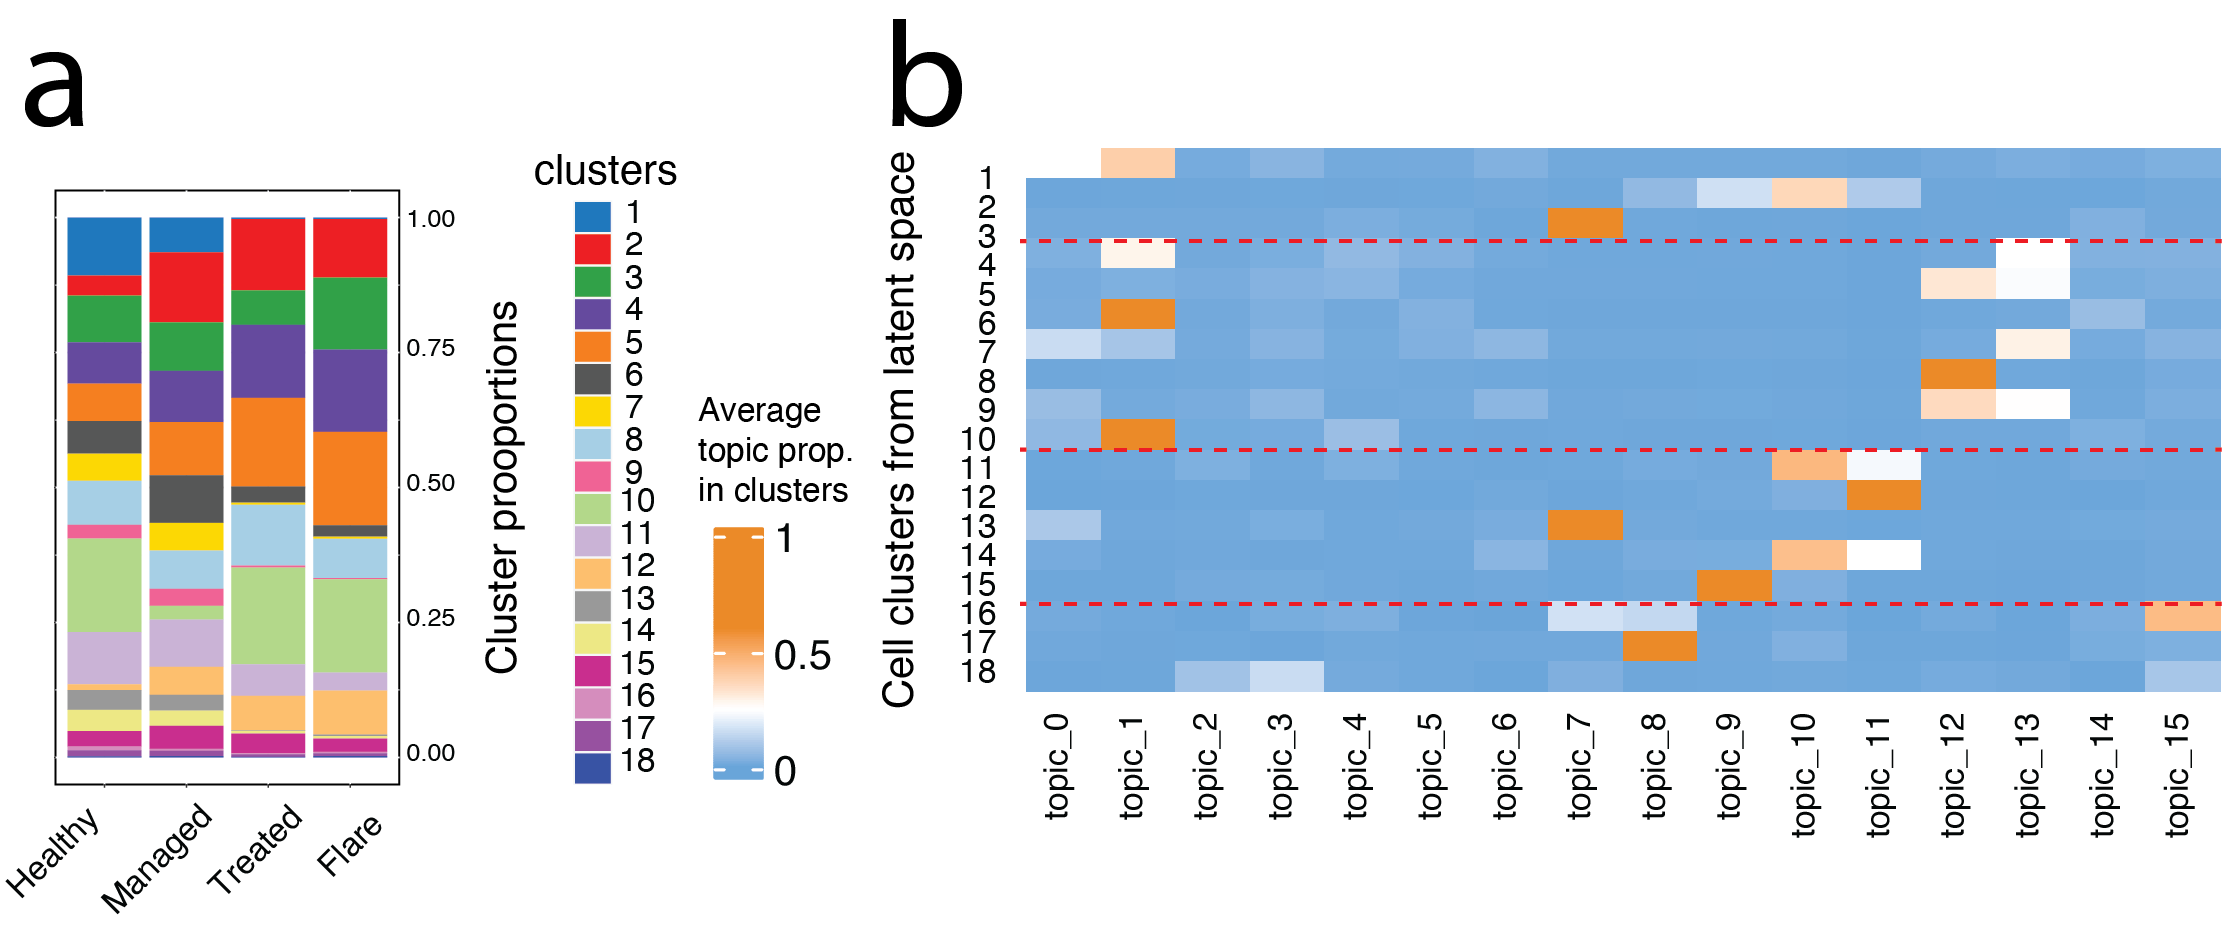
\includegraphics[width=\textwidth]{Figures/disease_strat_sftmx.png}
    \caption{\textbf{Cluster composition within samples is disease status dependent} a) Cell cluster proportion breakdown by SLE disease status shows cell composition within samples. b) Heatmap showing the median values of latent topic proportions across cells within each Louvain cluster. Clusters are shown along the rows of the heatmap.}
    \label{fig:diseasestrat}
\end{figure}

From the provided metadata of the scRNA-seq dataset in Perez \textit{et al.} \cite{sledata}, the trained model was analyzed in a disease-stratified fashion. Using the same Louvain clusters determined in the previous section (Fig.\ref{fig:cluster_umap}), differentially represented clusters were found depending on SLE disease status (Fig.\ref{fig:diseasestrat}a). Clusters 1, 6, 7, 9 and 11 capture primarily cells from healthy individuals or individuals with managed SLE. Cells in clusters 2 and 12 make up a significantly greater portion of cells from individuals with any level of SLE compared to healthy individuals. Some clusters make up a greater portion of cells from individuals with active disease phenotypes of SLE (treated vs. flare), such as clusters 4 and 5. Finally, cluster 10 appears in each condition except for individuals with managed SLE. The differences in cluster representation suggest that the cellular makeup of PBMCs is associated with disease status. 

To understand how each cluster relates to the estimated latent topic representation of cells, the average topic profile for cells in each cluster is constructed (Fig.\ref{fig:diseasestrat}b). From this, it is shown that many clusters that are differentially represented across disease conditions actually share many features, suggesting that cells in different clusters may correspond to the same general cell type, but have some minute differences in gene expression. For example, clusters 4 and 7 both have strong representations by topics 1 and 13 but cells in cluster 7 have a higher representation in topic 0. Cells in these clusters are shown to be most closely aligned with effector memory and regulatory CD4+ T cells (Fig.\ref{fig:cluster_ct}), yet are distinctly different in their latent topic profiles. 

\begin{figure}
    \centering
    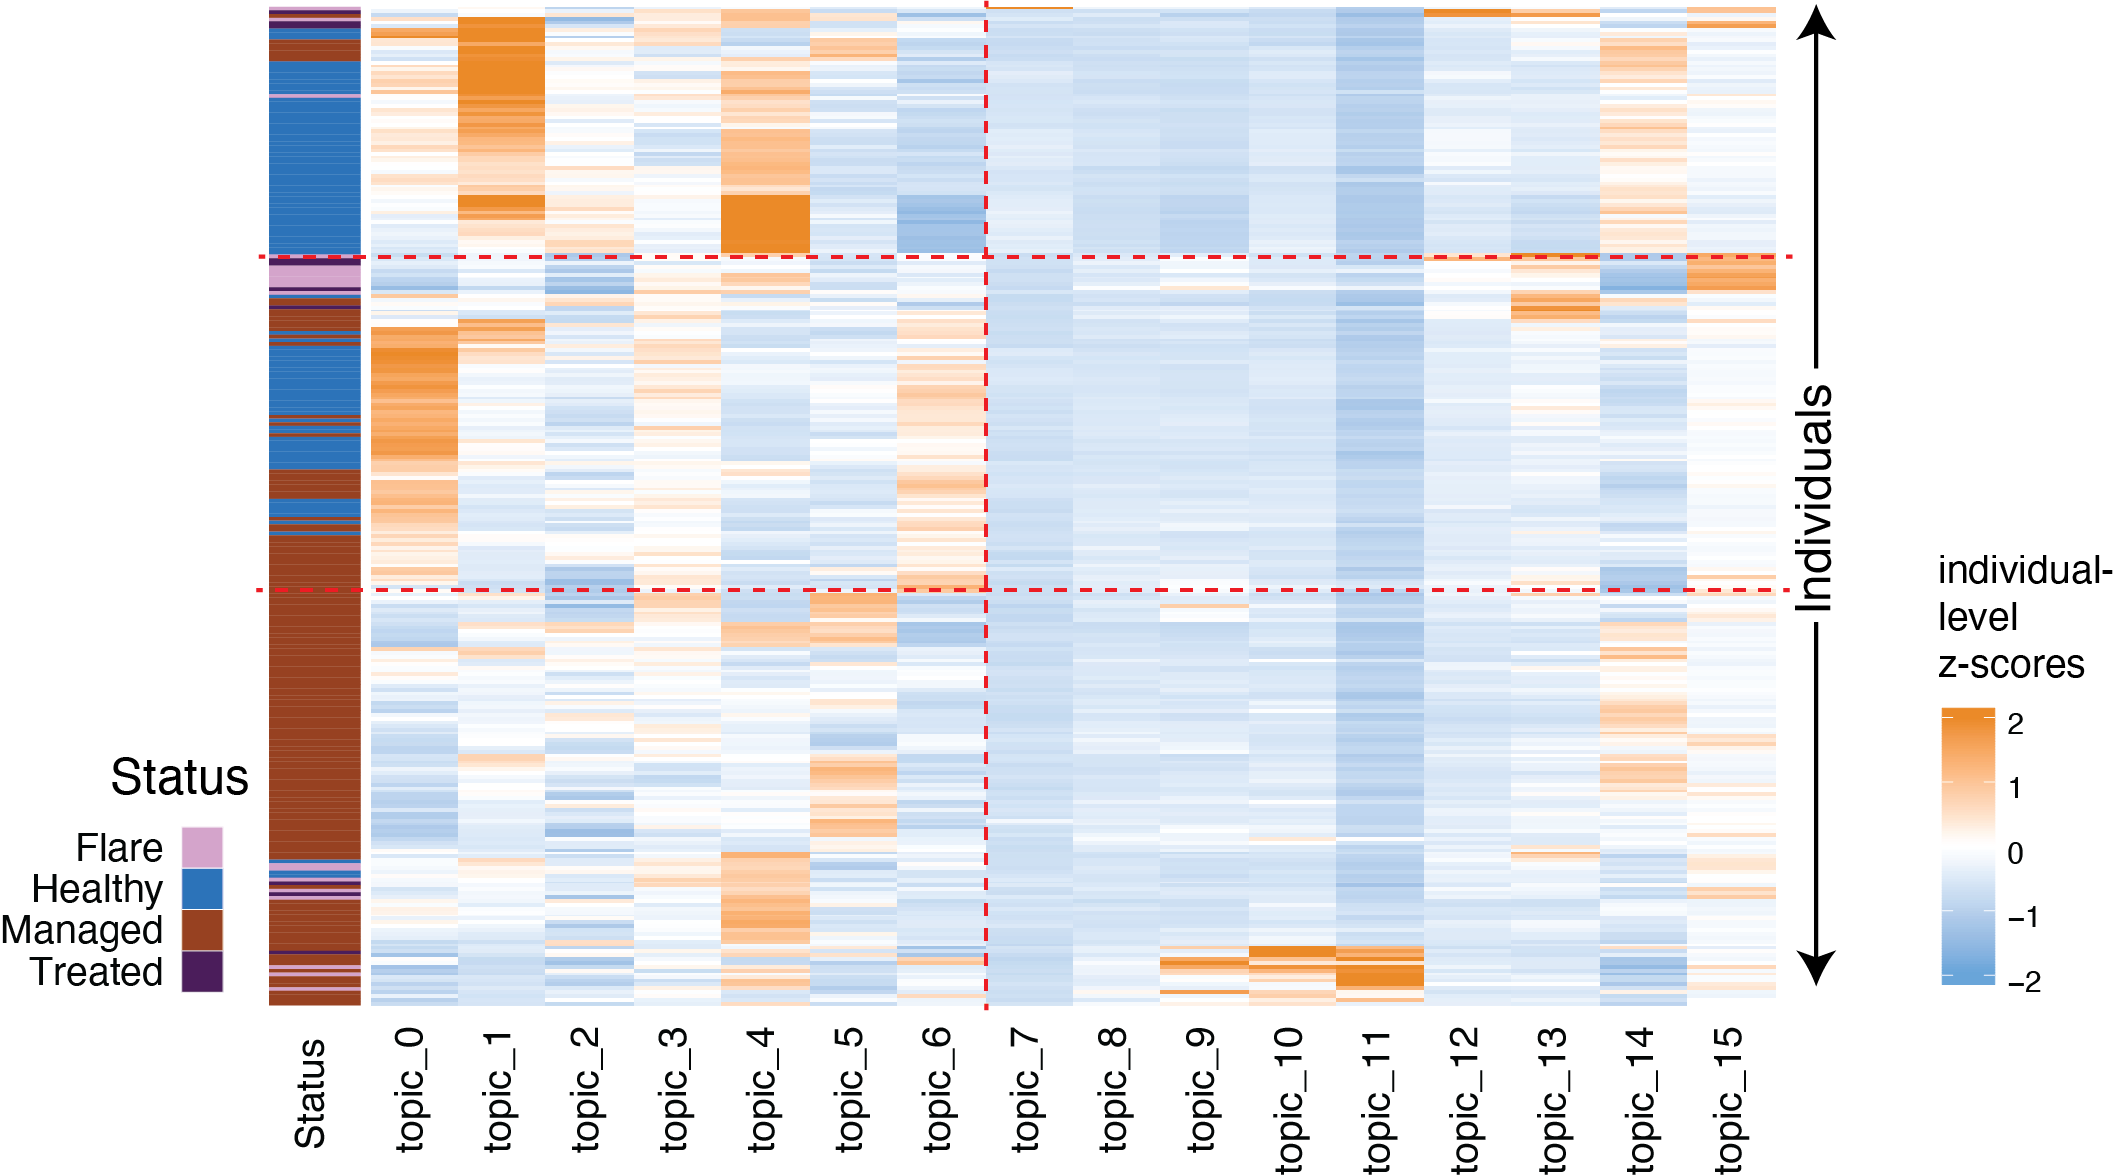
\includegraphics[width=\textwidth]{Figures/ind_median_latent_prof.png}
    \caption{\textbf{Individuals with identical disease status generally share latent topic patterns} Heatmap shows median latent topic profiles calculated for each individual included in the study. Rows represent each individual and are annotated by disease status.}
    \label{fig:ind_latent_prof}
\end{figure}

\begin{figure}
    \centering
    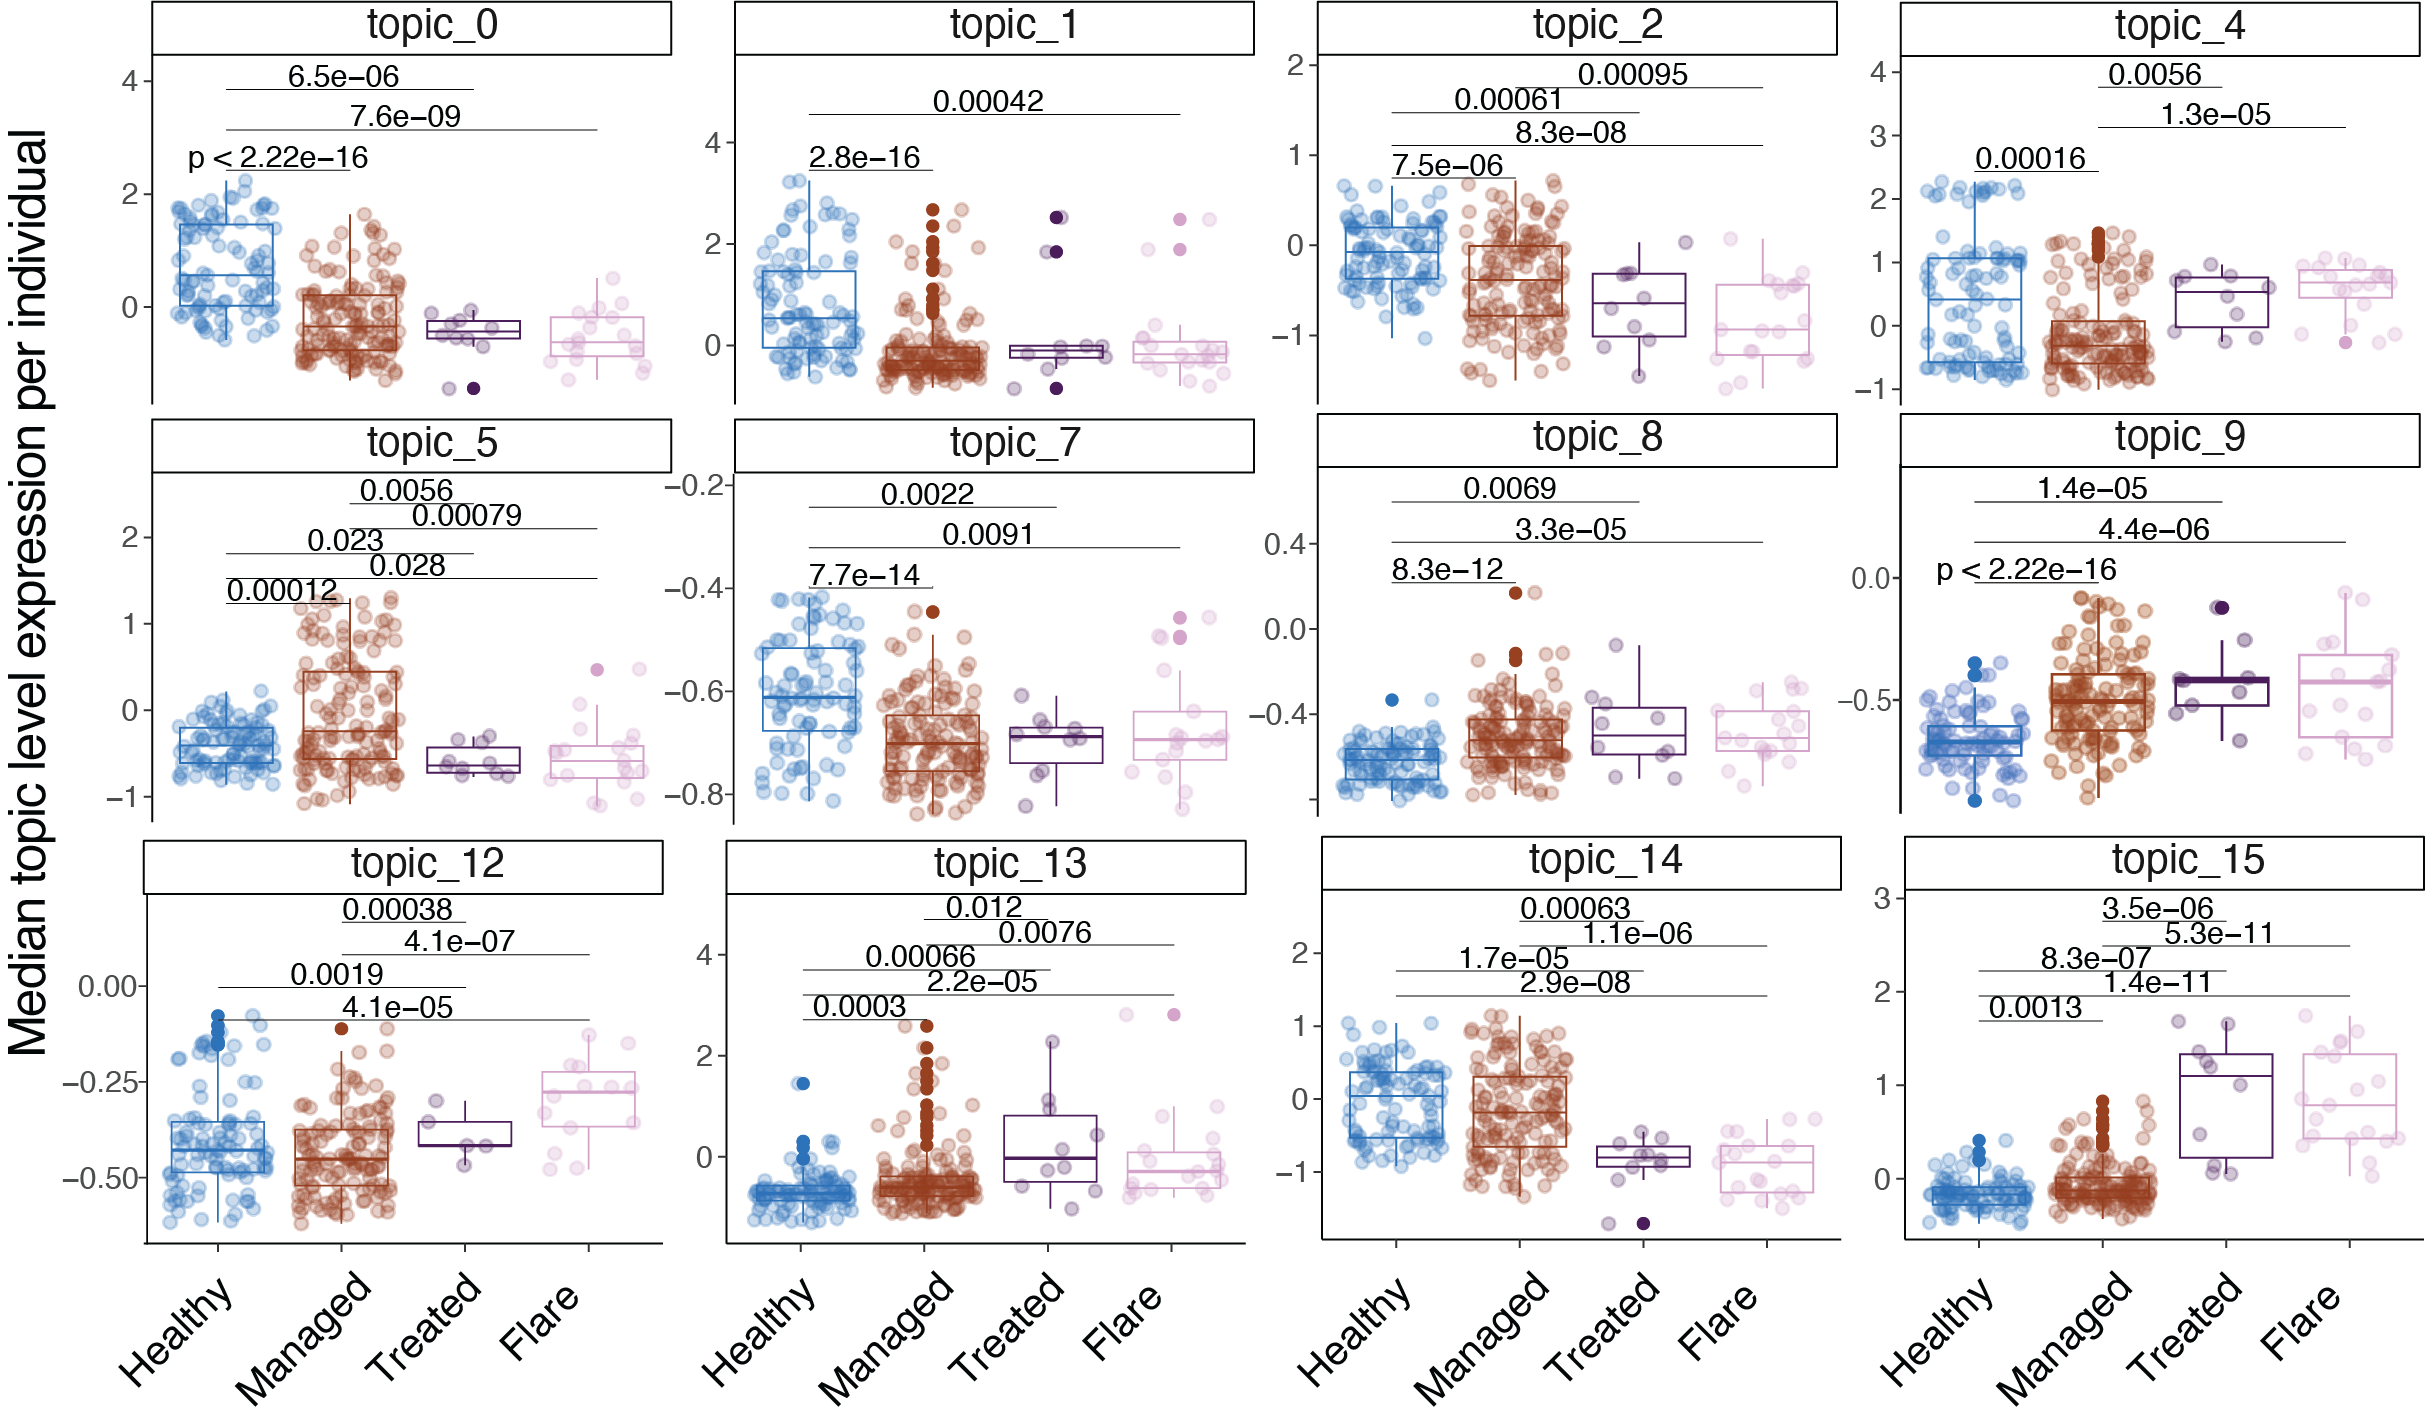
\includegraphics[width=\textwidth]{Figures/median_bxplt.png}
    \caption{\textbf{Disease status dependent differences exist in topic representation} Boxplots of median topic expressions per individual grouped by disease status. Topics with significant differences in median topic values between healthy and SLE individuals are shown. Significance between median expression values are calculated using Wilcoxon rank-sum tests between disease status individuals.}
    \label{fig:ind_bxplt}
\end{figure}

To better understand differences in topic representation as an effect of disease phenotype, the median topic profile for each individual included in the study is constructed (Fig.\ref{fig:ind_latent_prof}). From the latent profiles, a large variance in topic profiles across individuals is seen, yet individuals with similar profiles tend to share the same disease status. Wilcoxon rank-sum tests were performed on median latent topic values of individuals between disease status groups (Fig.\ref{fig:ind_bxplt}). Of note, topics 0 and 1 are  significantly differentially represented in healthy individuals compared to individuals with SLE of any status. Topic 0 separates cells found in cluster 7 from those in cluster 4, while topic 1 is seen in all clusters containing CD4+ T cells. Topic 12, which is represented in clusters corresponding to NK cells, CD8+ T cells and proliferating lymphocytes(Fig.\ref{fig:cluster_ct}, Fig.\ref{fig:diseasestrat}b), is significantly higher in individuals with treated and flare SLE conditions compared to healthy and managed SLE. Healthy individuals and those with managed SLE have a significantly higher level of topic 14 than those with an active SLE status, while the inverse is true for topic 15, suggesting a higher prevalence of intermediate immune cell states in individuals with active SLE while healthy and managed individuals have a higher prevalence of B cells and certain naive T lymphocytes (Fig.\ref{fig:cluster_ct}, Fig.\ref{fig:diseasestrat}b). Showing the differences in topic levels across disease statuses informs our investigation into the differentially regulated biological gene sets suggested by the latent-node level gene embeddings of the model. 

\newpage
\section{Functional Analysis of Latent Nodes}

\subsection{Node-level Gene Clustering}

\begin{figure}
    \centering
    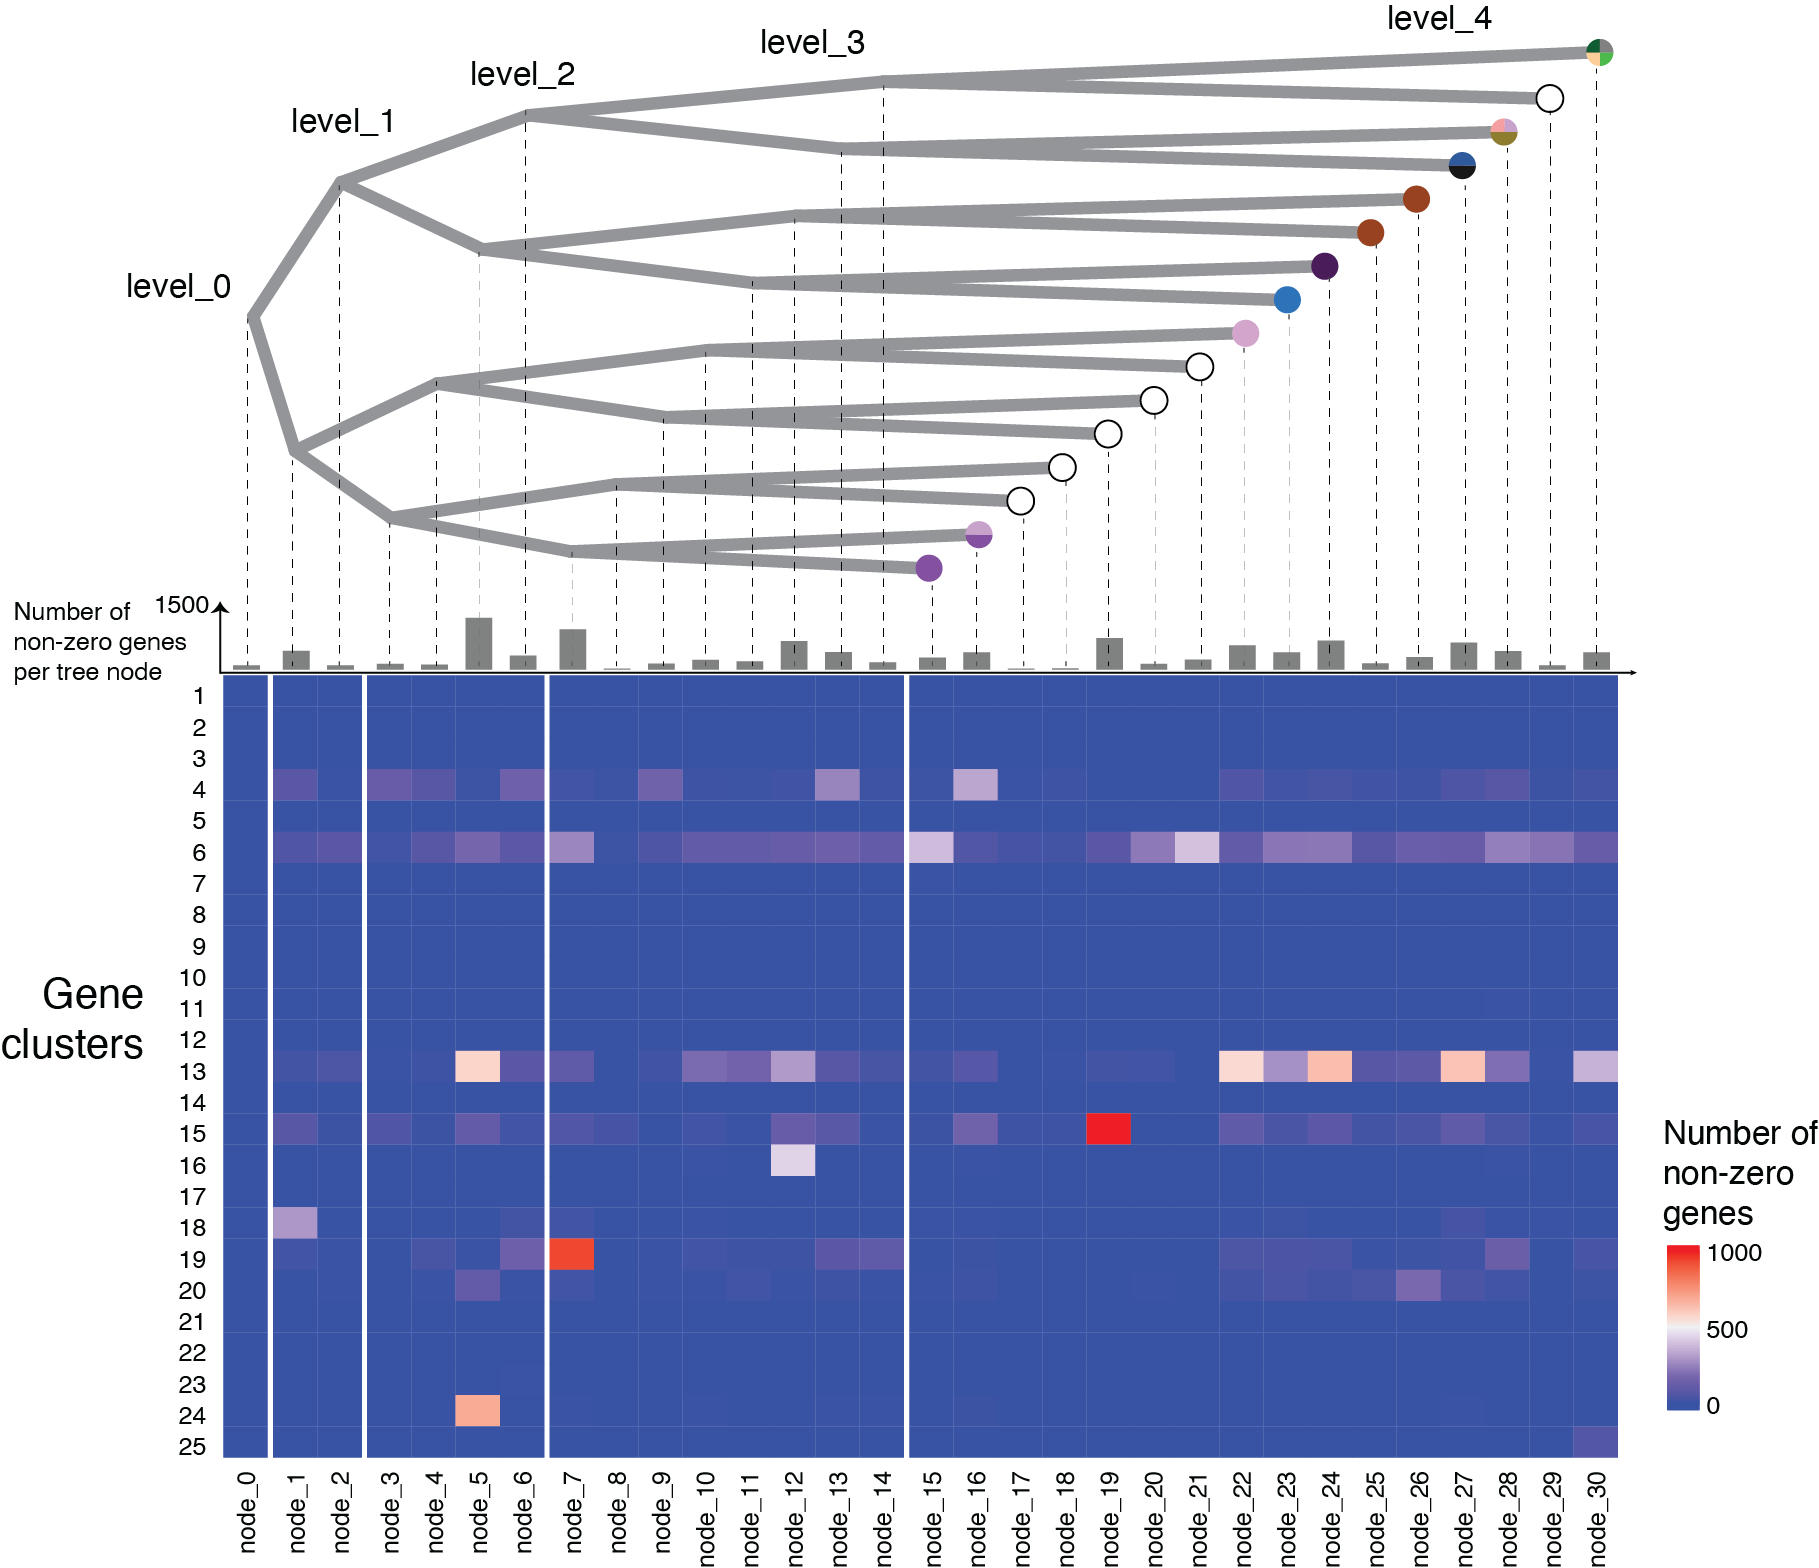
\includegraphics[width=\textwidth]{Figures/node_clusters.png}
    \caption{\textbf{Clustering of genes based on node-level embeddings show overarching gene programs} Heatmap shows number of significantly non-zero genes within each node that belong to gene clusters. Total numbers of non-zero genes per tree node are annotated above.}
    \label{fig:nodeanalysis}
\end{figure}

Further investigation was conducted on the number of genes that effectively define cell-type specific disease mechanisms using learned node-level gene vectors from LaRCH, namely $\hat{\beta}$ parameters before the tree-based topic-level aggregation. It is assumed that Bayesian variable selection prior can put zero values to unnecessary (or statistically weak) associations for irrelevant genes. Counting only the number of genes significantly deviating from zero, the number of genes needed for each tree node and level was counted (Fig. \ref{fig:nodeanalysis}). For brevity, genes were clustered into 25 distinctive gene modules by applying the Louvain clustering method on the 10-nearest neighbour gene-gene interaction graph (Fig.\ref{fig:nodeanalysis}). The Bayesian spike-and-slap prior ensured that the node-level gene programs are determined by a subset of genes between 50 to 1800 genes, with a median number of 429. Albeit, more genes were found on nodes 5 (cluster 24) and 7 (cluster 19), which correspond to T- and B-cell groups, respectively.

\subsection{Gene Set Enrichment Analysis of Node-Level Gene Embeddings}

\begin{figure}
    \centering
    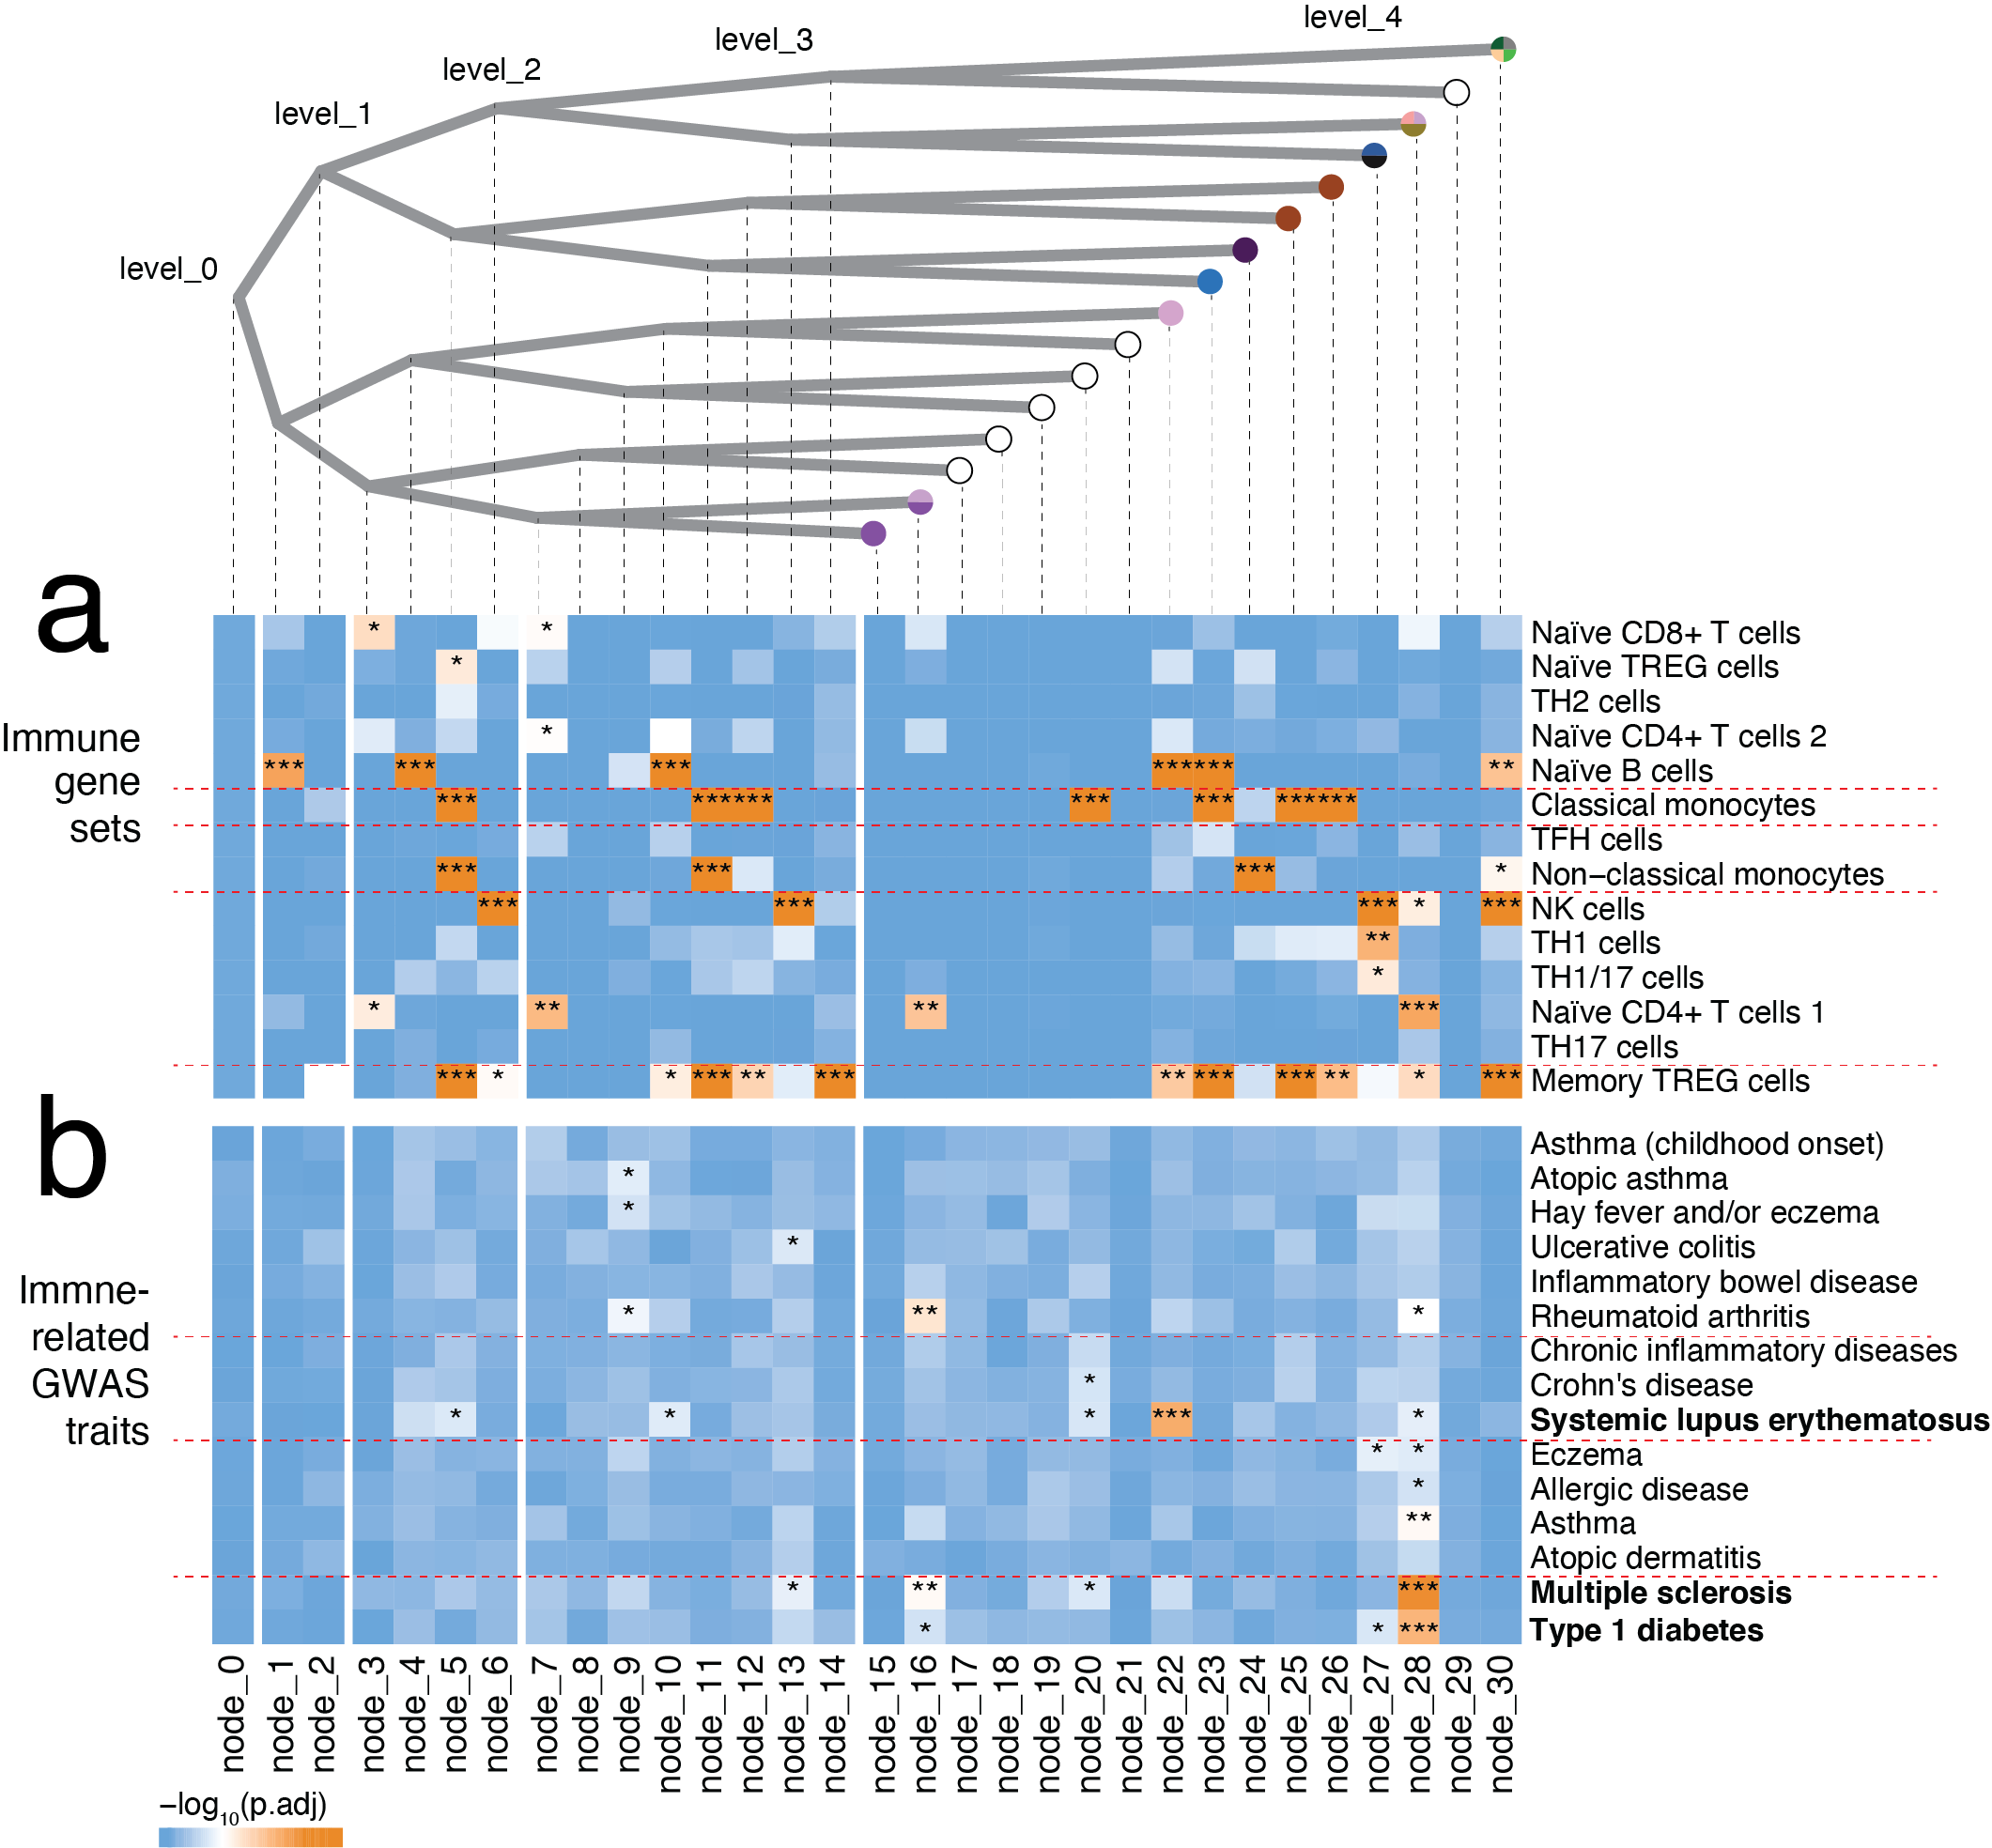
\includegraphics[width=\textwidth]{Figures/gsea.png}
    \caption{\textbf{Gene set enrichment analysis shows immune subset and disease relevant features described by latent node features} Heatmap shows the $-\log(p)$ enrichment significance of each gene set per node. Significance annotations are as follows: $*** - p < 0.0001, ** - p < 0.001, * - p < 0.01$.}
    \label{fig:gsea}
\end{figure}

Enrichment analysis of cell-type specific differentially expressed gene sets based on gene embedding values allows for further annotation of cell type relationships to latent topics. Ranked gene set enrichment analysis was performed using the \texttt{fgsea} R package \cite{fgsea} with the estimated embedding values $\hat{\beta}$ as the fgsea score. Gene sets used for enrichment analysis were obtained from the DICE database \cite{DICE1}, the NHGRI-EBI Catalog of human genome-wide association studies \cite{gwas_cat}, ImmuneSigDB \cite{godec2016compendium}, and the hallmark gene sets within MSigDB \cite{liberzon2015molecular}.

Gene sets related to immune function were found to be enriched in a number of relevant latnet nodes, suggesting functional phenotypic features represented through latent topic representation (Fig. \ref{fig:immune_gsea}). B cell-related genes are enriched at the early stages of the node tree, suggesting a distinct model lineage that these cells follow (Fig.\ref{fig:gsea}a). an enrichment of B cell-related genes in node 23 is also seen, along with classical monocyte and memory regulatory T cell-related genes. In Fig.\ref{fig:sle_tree}, topic 8 (made up of nodes 0, 2, 5, 11, and 23) was determined to correspond to dendritic cells, which canonically share lineage paths with both monocytes and lymphoid cells \cite{immunediff}. Topic 1 (made up of nodes 0, 1, 3, 7, and 16), which is significantly greater in healthy individuals (Fig.\ref{fig:ind_bxplt}), is enriched in genes relating to naive T cells, suggesting a loss of naive cells and concomitant increase in activated T cells in individuals with SLE. Gene sets of less prevalent sub-types, such as Th17 and Th2 helper T cell subsets, are not found to be significantly enriched in any node as they are difficult to distinguish amidst a heterogeneous sample. 

Enrichment analysis of GWAS (GWAS) gene sets pertaining to immunological disease reveals node-level differences in disease manifestation (Fig.\ref{fig:gsea}b). Disease-relevant gene sets are mainly found to be enriched in nodes at deeper levels of the tree, suggesting that disease manifestations are cell-type specific, rather than common features across many cells. GWAS genes relating to SLE are enriched primarily in node 22, which corresponds to topic 7. This node also is related to B cell function (Fig.\ref{fig:nodeanalysis}b), which is in line with the fact that SLE is often characterized by abnormal autoreactive B cells \cite{slebcells}. Node 28, corresponding to topic 13, is enriched in gene sets relating to other autoimmune diseases, such as multiple sclerosis and type-1 diabetes, as well as memory Treg cells, naive CD4+ T cells, and NK cells. Autoreactive T cell function is the primary driver of these diseases \cite{ms, t1d} and the corresponding topic 13 is enriched in individuals with SLE (Fig.\ref{fig:ind_bxplt}), suggesting an additional role of autoreactive T cells in SLE pathogenesis. 

\newpage
\section{Node-level Marker Genes}

Node-level gene embedding values allow for the identification of significant marker genes that contribute to the gene expression signature of cells represented by specific latent topics. From the node-level marker genes, biological meaning can be extracted to provide insight on cell-type specific features associated with SLE.

\subsection{Marker Gene Significance Testing}

Significant marker genes for each latent node were obtained using  parameters learned in the decoder component of LaRCH. $\hat{\beta}$ and $\mathbb{V}[\hat{\beta}]$, calculated using (\ref{eq:betahat_est}) and (\ref{eq:betahat_var}), were fed directly into the \texttt{ashr} R package described in the Stephens \textit{et al.} \cite{ashr}. This package uses an emprical Bayes approach for large-scale hypothesis testing and false discovery rate estimation. Significant genes are selected as those with \texttt{qvalue} $< 0.05$. The number of significant genes per node is detailed in table \ref{tab:sig_genes}. Unique significant genes are used to identify gene features that separate a specific latent tree node from its parent and sibling nodes, therefore playing a role in driving the differentiation from one topic path to another. A significant gene is considered unique to a node if it does not also appear as a significant gene it its parent a direct sibling node. These gene counts are summarized in table \ref{tab:unique_sig_genes}.

\subsection{Marker Genes of Interest}
\begin{figure}
    \centering
    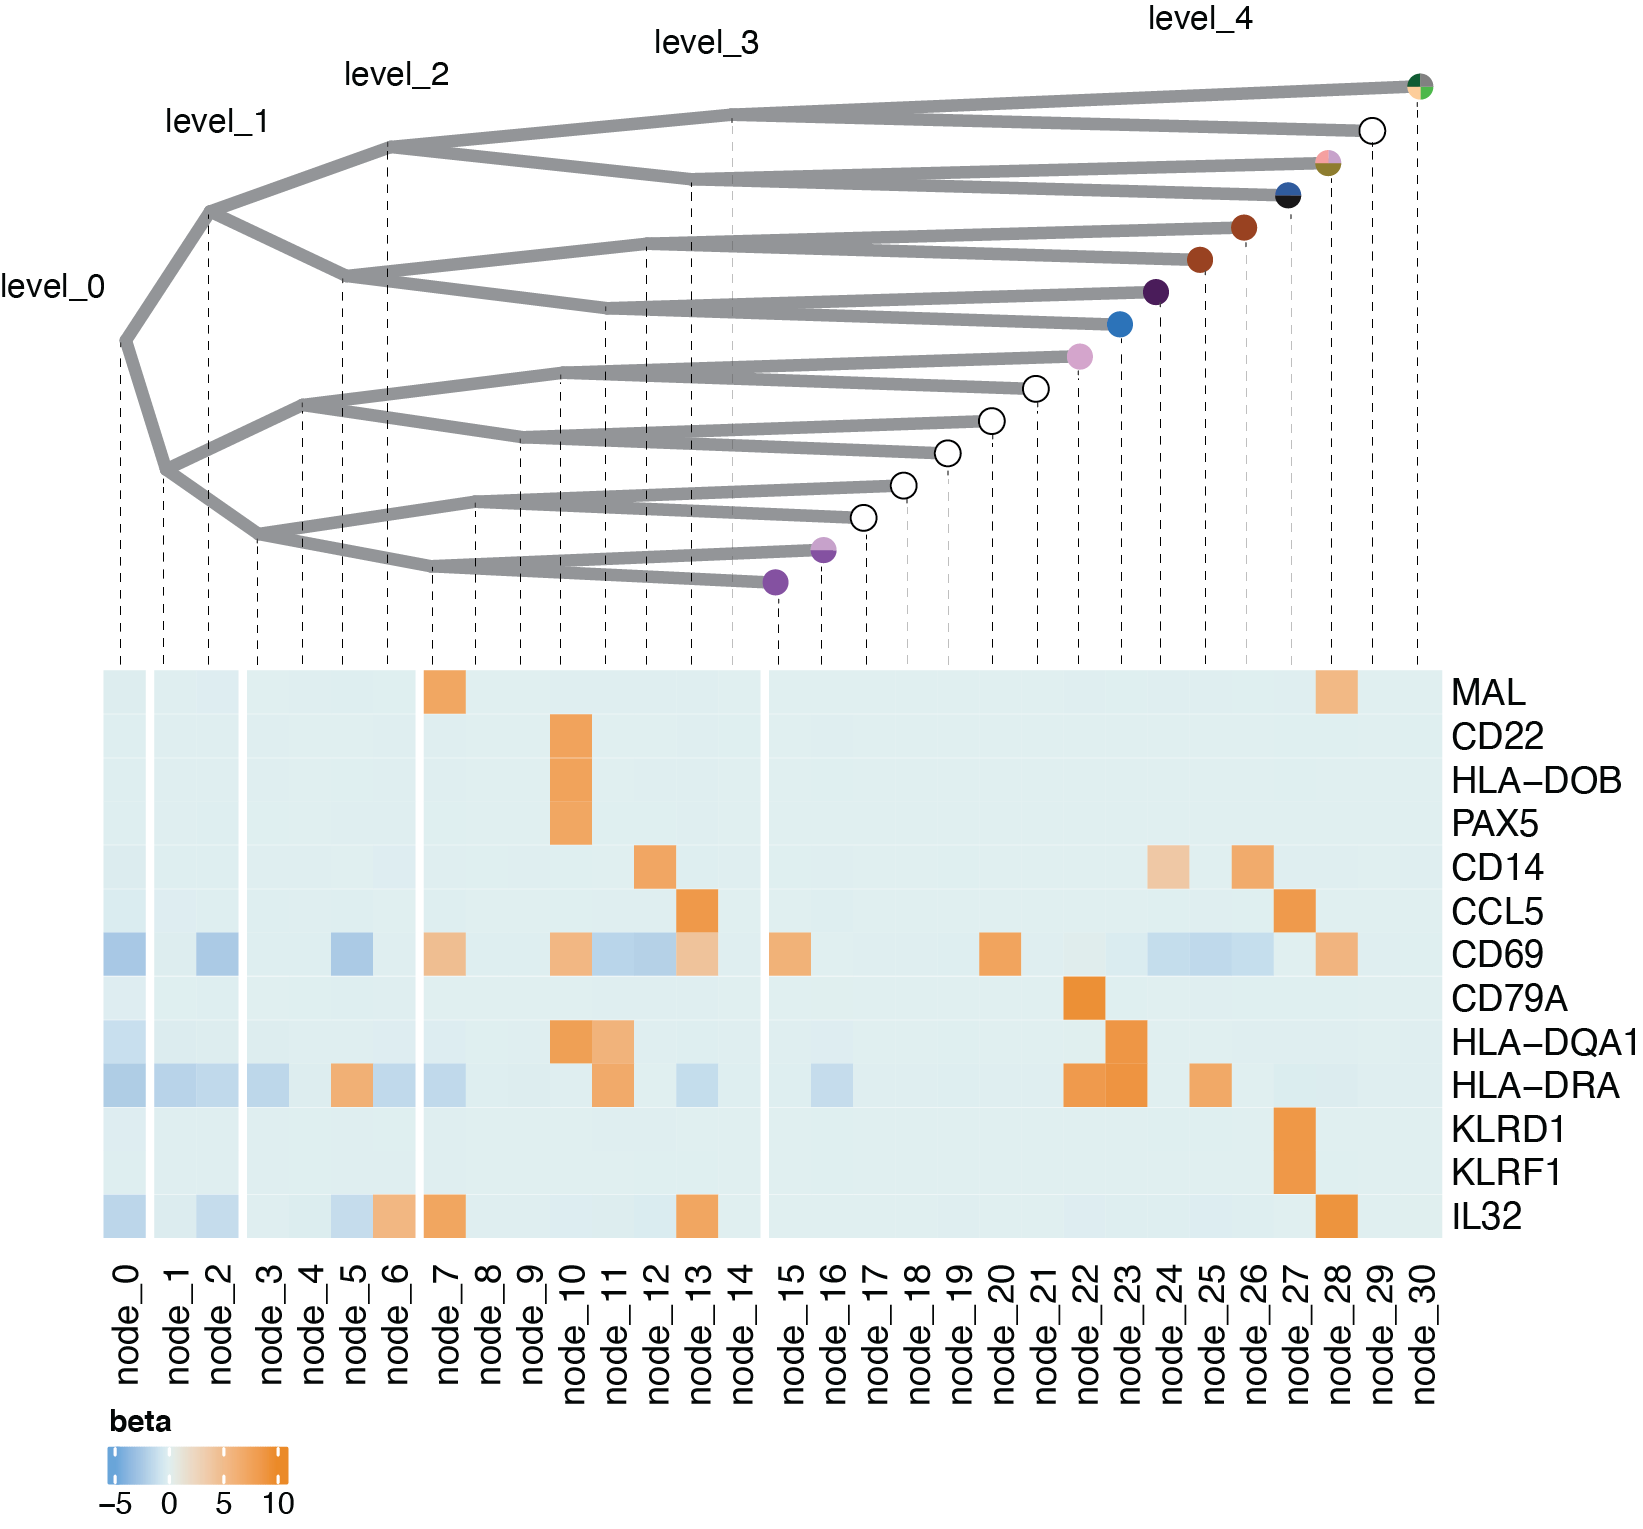
\includegraphics[width=\textwidth]{Figures/markers.png}
    \caption{\textbf{Canonical immune subset markers are captured in latent tree nodes of the topic model} Heatmap shows estimated node-wise gene embedding values $\hat{\beta}$ of genes previously identified as marker gene for immune cell subsets.}
    \label{fig:marker_genes}
\end{figure}

From the list of significant genes for each tree node, the top ten genes with the greatest absolute $\hat{\beta}$ value from each node are selected for further investigation. The top 80 genes from this list are shown in figure \ref{fig:top_beta_hm}.

\subsubsection{Significant Node-level Immune Marker Genes}
Within this list are several known immune cell type markers (Fig. \ref{fig:marker_genes}). 

MAL is a protein coding gene that is selectively expressed during T cell differentiation \cite{alonso1987cdna}. It is seen in  nodes 7 and 28, which correspond to topics 0, 1, and 13. This is in accordance with the labeling of these topics as representing T cell subsets in figure \ref{fig:sle_tree}. CD69 is a membrane-bound type II C-lectin receptor and is a marker of lymphocyte activation \cite{cibrian2017cd69}. It is identified as a marker gene in a number of nodes, all which correspond to topics containing lymphocyte subsets (0, 1, 7, 12, 13). Interestingly, this gene is also down regulated in nodes associated with monocyte subsets.

NK cells are identified by KLRD1 and KLRF1, two killer cell lectin like receptors which are markers of node 27, the leaf node of topic 12 \cite{cozar2021tumor}.

In nodes corresponding to topic 7, which is almost exclusively present in B cells, a number of B cell markers are present. In node 10 and 22, the two final nodes in the path of topic 7, CD22, HLA-DOB, PAX5, and CD79a are uniquely expressed in B cells. \cite{moyron2002expression, nagarajan2002class, chu2001cd79, desouki2010pax} HLA-DRA is identified as a marker gene in node 22 along with a number of other tree nodes that correspond with topics 8-11 which are associated with dendritic cells and monocytes. HLA-DRA is a HLA class II molecule that is a component of the major histocompatibility complex (MHC) II and is expressed on the surface of various antigen presenting cells (APCs) including B lymphocytes, dendritic cells, and monocytes \cite{VANDENELSEN200467}. CD14, a well known marker of monocyte \cite{goyert1986biochemistry}, is a top gene in nodes 12, 24, and 26 which correspond to topics 9, 10, and 11, topics associated with monocytes. 

From the analysis in this chapter, node-level immune cell markers are congruent with cell type assignments presented in Perez \textit{et al.} \cite{sledata}. The presentation of immune cell type marker genes as significant genes in tree nodes demonstrates the ability for the LaRCH model results to inform cell type assignments to scRNA-seq datasets using their latent topic representations. 

\subsubsection{Significant Node-level Genes with Potential SLE Disease Association}
\label{cha:genes}
\begin{figure}
    \centering
    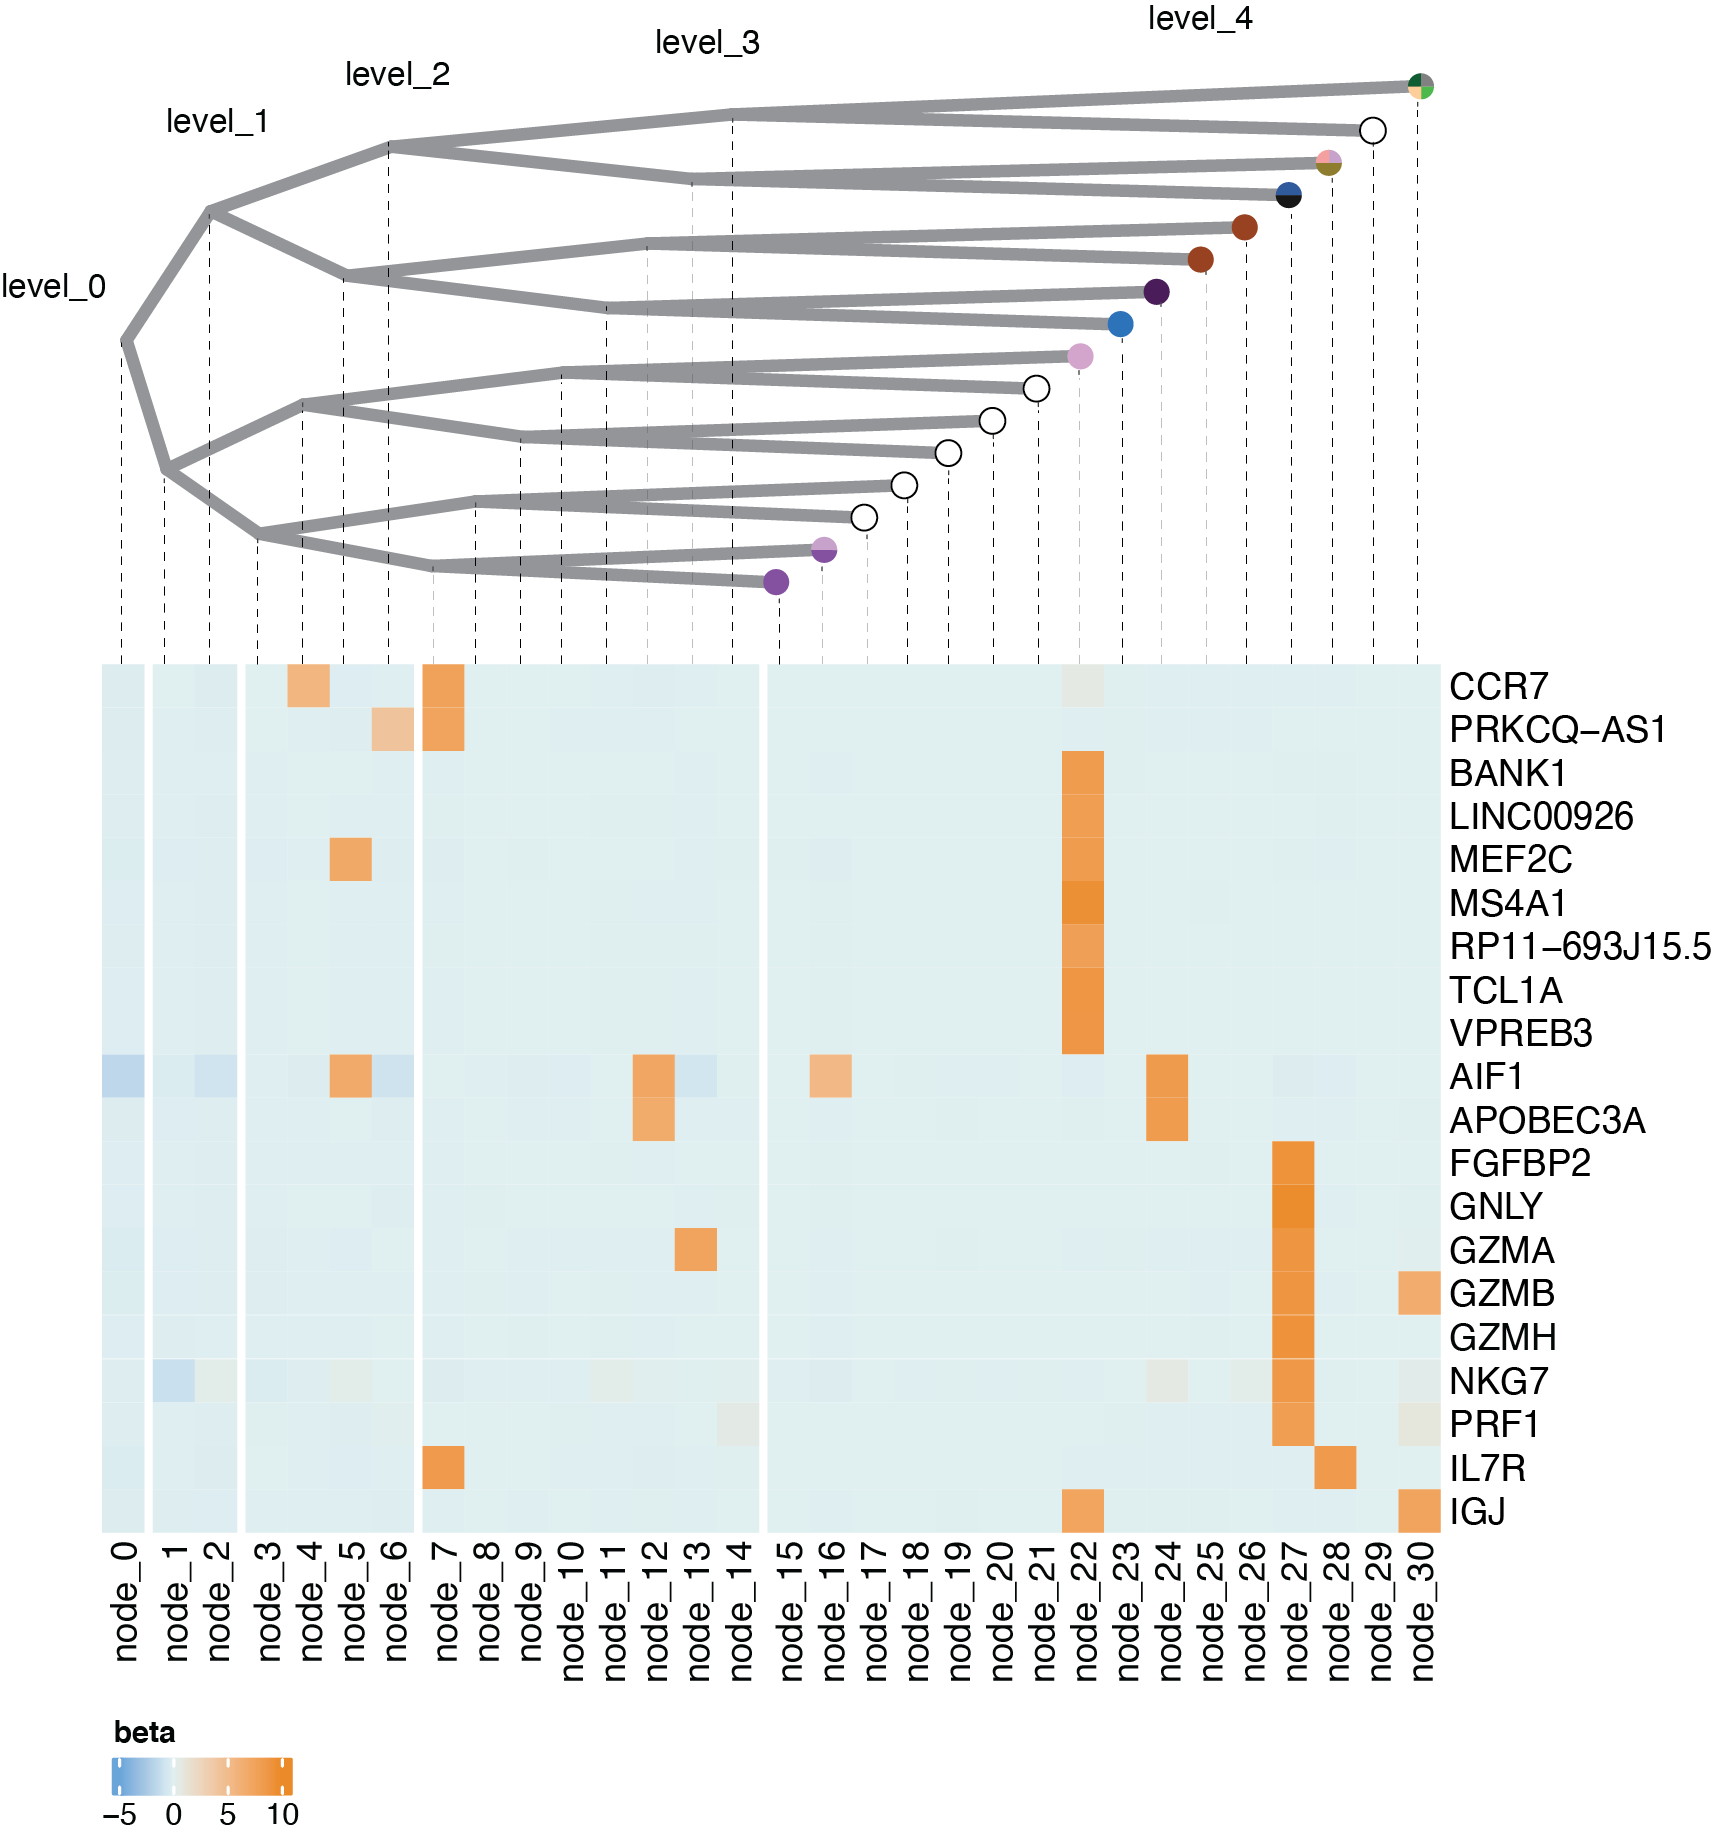
\includegraphics[width=\textwidth]{Figures/immune_genes.png}
    \caption{\textbf{Node-level gene embeddings reveal potential genes of interest with regards to SLE pathogenesis} Heatmap shows estimated node-wise gene embedding values $\hat{\beta}$ of genes with relevant immune function to SLE disease mechanisms.}
    \label{fig:immune_genes}
\end{figure}

Analysis of significant genes outside of canonical immune subset markers paired with the SLE disease status dependent differential topic representation provides insight into potential cell-type specific mechanisms associated with disease phenotypes. 

Patients experiencing SLE flares show significantly elevated representation of topic 12 \ref{fig:ind_bxplt}. This topic is associated with CD8+ T lymphocytes and nodes in this topic contain GZMH, GZMB, and PRF1 as marker genes. It has been shown that patients with SLE show elevated levels of GZMH+ cytotoxic CD8+ T cells \cite{sledata}. Similarly, PRF1 and GZMB expressing CD8+ T cells have been correlated with SLE disease activity \cite{blanco2005increase}. 

Topic 7, which contains node 22, has a significantly lower representation in patients with SLE. Node 22 has a number of significant genes associated with B cell function, including BANK1. BANK1 encodes a scaffolding protein expressed predominantly in B cells. Variants in this gene have been shown to elevate risk of SLE by increasing susceptibility to autoantibodies \cite{dam2016bank1}.

Patients with SLE show elevated representation in topic 9. The corresponding nodes of this topic, nodes 12 and 24 contain AIF1 and APOBEC3A as significant genes. AIF1 has been shown to be linked with the activation of macrophages and is implicated in several inflammatory diseases \cite{de2023aif1}, making it a viable candidate for exploration of macrophage related mechanisms driving SLE. APOBEC3A is a part of the APOBEC3 family of cytidine deaminase. APOBEC3A gene expression is induced by type I interferon (IFN-I) response during viral infections and plays an important role in defence against viral infection \cite{taura2022apobec3a}. Patients with SLE have been shown to have elevated expression of APOBEC3A compared to healthy controls, especially in those with flares \cite{perez2021sustained} and there is justification for further exploration into the role it plays in autoimmune disease \cite{liu2023underexplored}.

Topics 0 and 1 latent values are significantly higher in healthy individuals than patients with SLE \ref{fig:ind_bxplt}. A shared node in the paths of these topics is node 7 which contains the marker genes CCR7 and PRKCQ-AS1. CCR7 is a chemokine receptor that is critical to the function of naïve T cells \cite{britschgi2008dynamic}. This suggests an expected reduction of naïve CD4+ T cells in patients with SLE. PRKCQ-AS1 is a long non-coding RNA (lncRNA) that has recently been associated with the regulation of the expression of IL-1$\beta$, IL-6, and IL-8 in fibroblasts with TNF-$\alpha$ stimulation \cite{zhao2023role}, as well as the regulation of glycolysis and mitochondrial functions in thyroid carcinoma \cite{zhang2023fasting}. SNPs in this gene have also been associated with asthma, eczema, and allergic rhinitis \cite{shi2023characterization}, making it a viable candidate for exploration in the context of CD4+ T cell driven SLE manifestation. 






\chapter{Conclusion}
\section{Summary of Findings}
In this thesis, we present LaRCH, a neural topic model with a built-in node tree structure that enforces hierarchical relationships between latent topics through shared additive embedding features. A spike-and-slab prior informed gene embedding model parameters and provides a natural method of marker gene selection and the ability to perform interpretable latent feature detection. From multiple tests on realistic simulated scRNA-seq datasets, we show that LaRCH is effective at cell type discrimination in heterogeneous samples of immune cell gene expression profiles. By enforcing an underlying topic structure, we allow for an intuitive representation of nested relationships between cell types with shared lineage paths. 

Application of LaRCH on a single-cell gene expression dataset across multiple disease phenotypes of systemic lupus erythematosus shows disease dependent hierarchical genomic features. Our findings show cell type specific differences in gene expression in individuals with SLE in addition to overarching cellular features present across all cell types, suggesting disease mediated altered immune function. Investigation into specific node-level marker genes shows the detection of canonical immune subset gene markers and genes with significant roles in immune function. Specifically, we detect differences in the expression of APOBEC3A in monocyte cell populations and PRKQ-AS1 in CD4+ T lymphocyte populations. APOBEC3A is an enzyme encoding gene that has been shown to be upregulated in patients with SLE, while PRKQ-AS1 is a lncRNA that has recently been associated with aberrant immune function and may play a key role in immunological disorders. Both genes show potential impact on the disease mechanisms of SLE and other autoimmunological disorders and are promising avenues for further investigation.

\section{Limitations}

The use cases of the LaRCH model are limited to samples of heterogeneous cell populations with highly variable gene features. Granularity of cell type detection proves to be a challenge and cell subsets with large overlapping gene expression profiles are difficult to discern from one another. Training a model with a deeper latent tree did not yield better results in this aspect. This means that the application of this model would not be suitable for several uses cases such as constructing cancer phylogenies or the detection of rare cell subsets, where detection of minute differences is necessary.
 
Using a fixed perfect binary tree structure may lead to over parameterization of the model where many components of the tree are unused, resulting in an ill-fitting tree structure to represent the data. Unfortunately, including a tree-fitting component to the model would greatly increase computational burden as the search space would be super-exponential. \textit{Post-hoc} tree pruning could help solve this problem, but would result in the loss of information in the model. In LaRCH, we combat over-fitting at the embedding parameter level by implementing Bayesian priors that encourage model sparsity.

Training of the LaRCH model requires intensive computational resources. LaRCH is implemented in Python using a machine-learning library (\texttt{PyTorch} \cite{pytorch}), which often has specialized requirements for hardware, such as graphics processing units (GPUs), with sufficient processing capabilities and memory capacity. All model training experiments presented in this thesis were executed on a Nvidia Linux X64 Display Driver GPU. Smaller scRNA-seq datasets of 2,000 cells across ~50,000 genes requires on average 12 minutes to complete model training with a tree depth of 5 in 1,000 epochs. However, on a large gene expression dataset of 1.2 million cells across ~30,000 genes, training required over 60 hours to complete.

\section{Future Directions}
The LaRCH model may be readily expanded to include other HTS data types. Integration of ChIP-seq data of transcription factor binding affinity or ATAC-seq data of DNA accessibility profiles would be natural additions to this model. Multi-omic integration could provide valuable insights into the gene mechanistic drivers of cell type differentiation. 

To understand overall trends in up and down-regulated gene sets, one could relax element-wise sparsity in facour of set-wise sparsity and fine-mapping of genes, building upon the Sum of Single Effects (SuSiE) method of variable selection outlined in Wang \textit{et al.} \cite{susie}. Such a formulation would likely result in a more scalable iterative coordinate-wise algorithm, while assigning high probability mass on causal/anchor features for each independent effect. In fact, implementing a tree-structured latent feature space is also a promising extension to less computationally intensive factorization-based learning algorithms such as NMF. Such algorithms are able to yield low-dimensional embeddings of genomic data, maintaining many use cases of a neural topic model, in an more computationally efficient manner. 

Finally, using the results of the LaRCH model, a number of validation experiments can be performed. From the genes described in Chapter \ref{cha:genes}, genetic perturbation experiments on healthy and disease models to uncover the downstream effects of differential expression of these genes. From these experiments, there is a potential for bettering our understanding of mechanisms of immune function involved in driving the pathogenesis of autoimmune disorders including SLE.

%% This file is setup to use a bibtex file sample.bib and uses the
%% plain style.  Other styles may be used depending on the conventions
%% of your field of study.
%%
%%% Note: the bibliography must come before the appendices.
\renewcommand\bibname{References}
\bibliographystyle{ieeetr}
\bibliography{sample}

%% Use this to reset the appendix counter.  Note that the FoGS
%% requires that the word ``Appendices'' appear in the table of
%% contents either before each appendix lable or as a division
%% denoting the start of the appendices.  We take the latter option
%% here.  This is ensured by making the \texttt{appendicestoc} option
%% a default option to the UBC thesis class.

%%% If you only have one appendix, please uncomment the following line.
% \renewcommand{\appendicesname}{Appendix}
\appendix
\chapter{Supplementary Tables and Figures}
\begin{sidewaystable}[]
\centering
\begin{tabular}{|c|c|c|c|c|c|c|}
\hline
\multicolumn{7}{|c|}{Th1} \\
 \hline
        Study & $\alpha$ CD3 & $\alpha$ CD28 & IL-2 & IL-12 & TNF-$\alpha$ & $\alpha$ IL-4\\
        \hline
        Field 2020 \cite{Field2020} & 5 $\mu$g/mL & 0.5 $\mu$g/mL & 100 U/mL & 10 ng/mL & 10 $\mu$g/mL & \textemdash\\
        Bailis 2019 \cite{Bailis2019} & beads & beads & 5 ng/mL & 2 ng/mL & 10 $\mu$g/mL & \textemdash\\
        Sallin 2017 \cite{Sallin2017} & 3 $\mu$g/mL & 1 $\mu$g/mL & 0.12-30 ng/mL & 0.12-30 ng/mL & 10 $\mu$g/mL & \textemdash\\
        Yang 2019 \cite{Yang2019} & 1 $\mu$g/mL & 1 $\mu$g/mL & \textemdash & 10 ng/mL & 5 $\mu$g/mL & 100 ng/mL\\
        Thomas 2012 \cite{Thomas2012} & 1 $\mu$g/mL & 1 $\mu$g/mL & \textemdash & 10 ng/mL & 10 $\mu$g/mL & \textemdash\\
        Jiang 2018 \cite{Jiang2018} & 5 $\mu$g/mL & 5 $\mu$g/mL & \textemdash & 10 ng/mL & 10 $\mu$g/mL & \textemdash\\
        Pham 2014 \cite{Pham2014} & 2 $\mu$g/mL & 0.5 $\mu$g/mL & \textemdash & 5 ng/mL & 10 $\mu$g/mL & \textemdash\\
        Wagner 2021 \cite{Wagner2021} & 1 $\mu$g/mL & 1 $\mu$g/mL & \textemdash & 20 ng/mL & \textemdash & \textemdash\\
        Puleston 2021 \cite{Puleston2021} & 5 $\mu$g/mL & 2 $\mu$g/mL & 100 U/mL & 10 ng/mL & 4 $\mu$g/mL & \textemdash\\
        \hline
        \multicolumn{7}{|c|}{Th2} \\
        \hline
        Study & $\alpha$ CD3 & $\alpha$ CD28 & IL-2 & IL-4 & $\alpha$ IL-12 & $\alpha$ IFN$\gamma$\\
        \hline
        Field 2020 \cite{Field2020} & 5 $\mu$g/mL & 0.5 $\mu$g/mL & 100 U/mL & 10 ng/mL & 10 $\mu$g/mL & 10 $\mu$g/mL\\
        Angela 2016 \cite{Angela2016} & \textemdash & \textemdash & 25 U/mL & 10 U/mL & \textemdash & 1 $\mu$g/mL\\
        Thomas 2012 \cite{Thomas2012} & 1 $\mu$g/mL & 1 $\mu$g/mL & \textemdash & 40 ng/mL & 10 $\mu$g/mL & 10 $\mu$g/mL\\
        Jiang 2018 \cite{Jiang2018} & 5 $\mu$g/mL & 5 $\mu$g/mL & \textemdash & 10 ng/mL & \textemdash & 10 $\mu$g/mL\\
        Pham 2014 \cite{Pham2014} & 2 $\mu$g/mL & 0.5 $\mu$g/mL & \textemdash & 10 ng/mL & \textemdash & 10 $\mu$g/mL\\
        Wagner 2021 \cite{Wagner2021} & 1 $\mu$g/mL & 1 $\mu$g/mL & \textemdash & 20 ng/mL & \textemdash & \textemdash\\
        Puleston 2021 \cite{Puleston2021} & 5 $\mu$g/mL & 2 $\mu$g/mL & 100 U/mL & 10 ng/mL & \textemdash & 4 $\mu$g/mL\\
        \hline
\end{tabular}
\caption{\textbf{Table summary of CD4+ polarization conditions} A meta-analysis of various studies with \textit{in vitro} CD4+ subset polarization condition protocols. Included are the polarization conditions for Th1s and Th2s across 10 studies. Units are presented as described in the original studies.}
\label{tab:CD4polarizationSupp}
\end{sidewaystable}

\begin{figure}
    \centering
    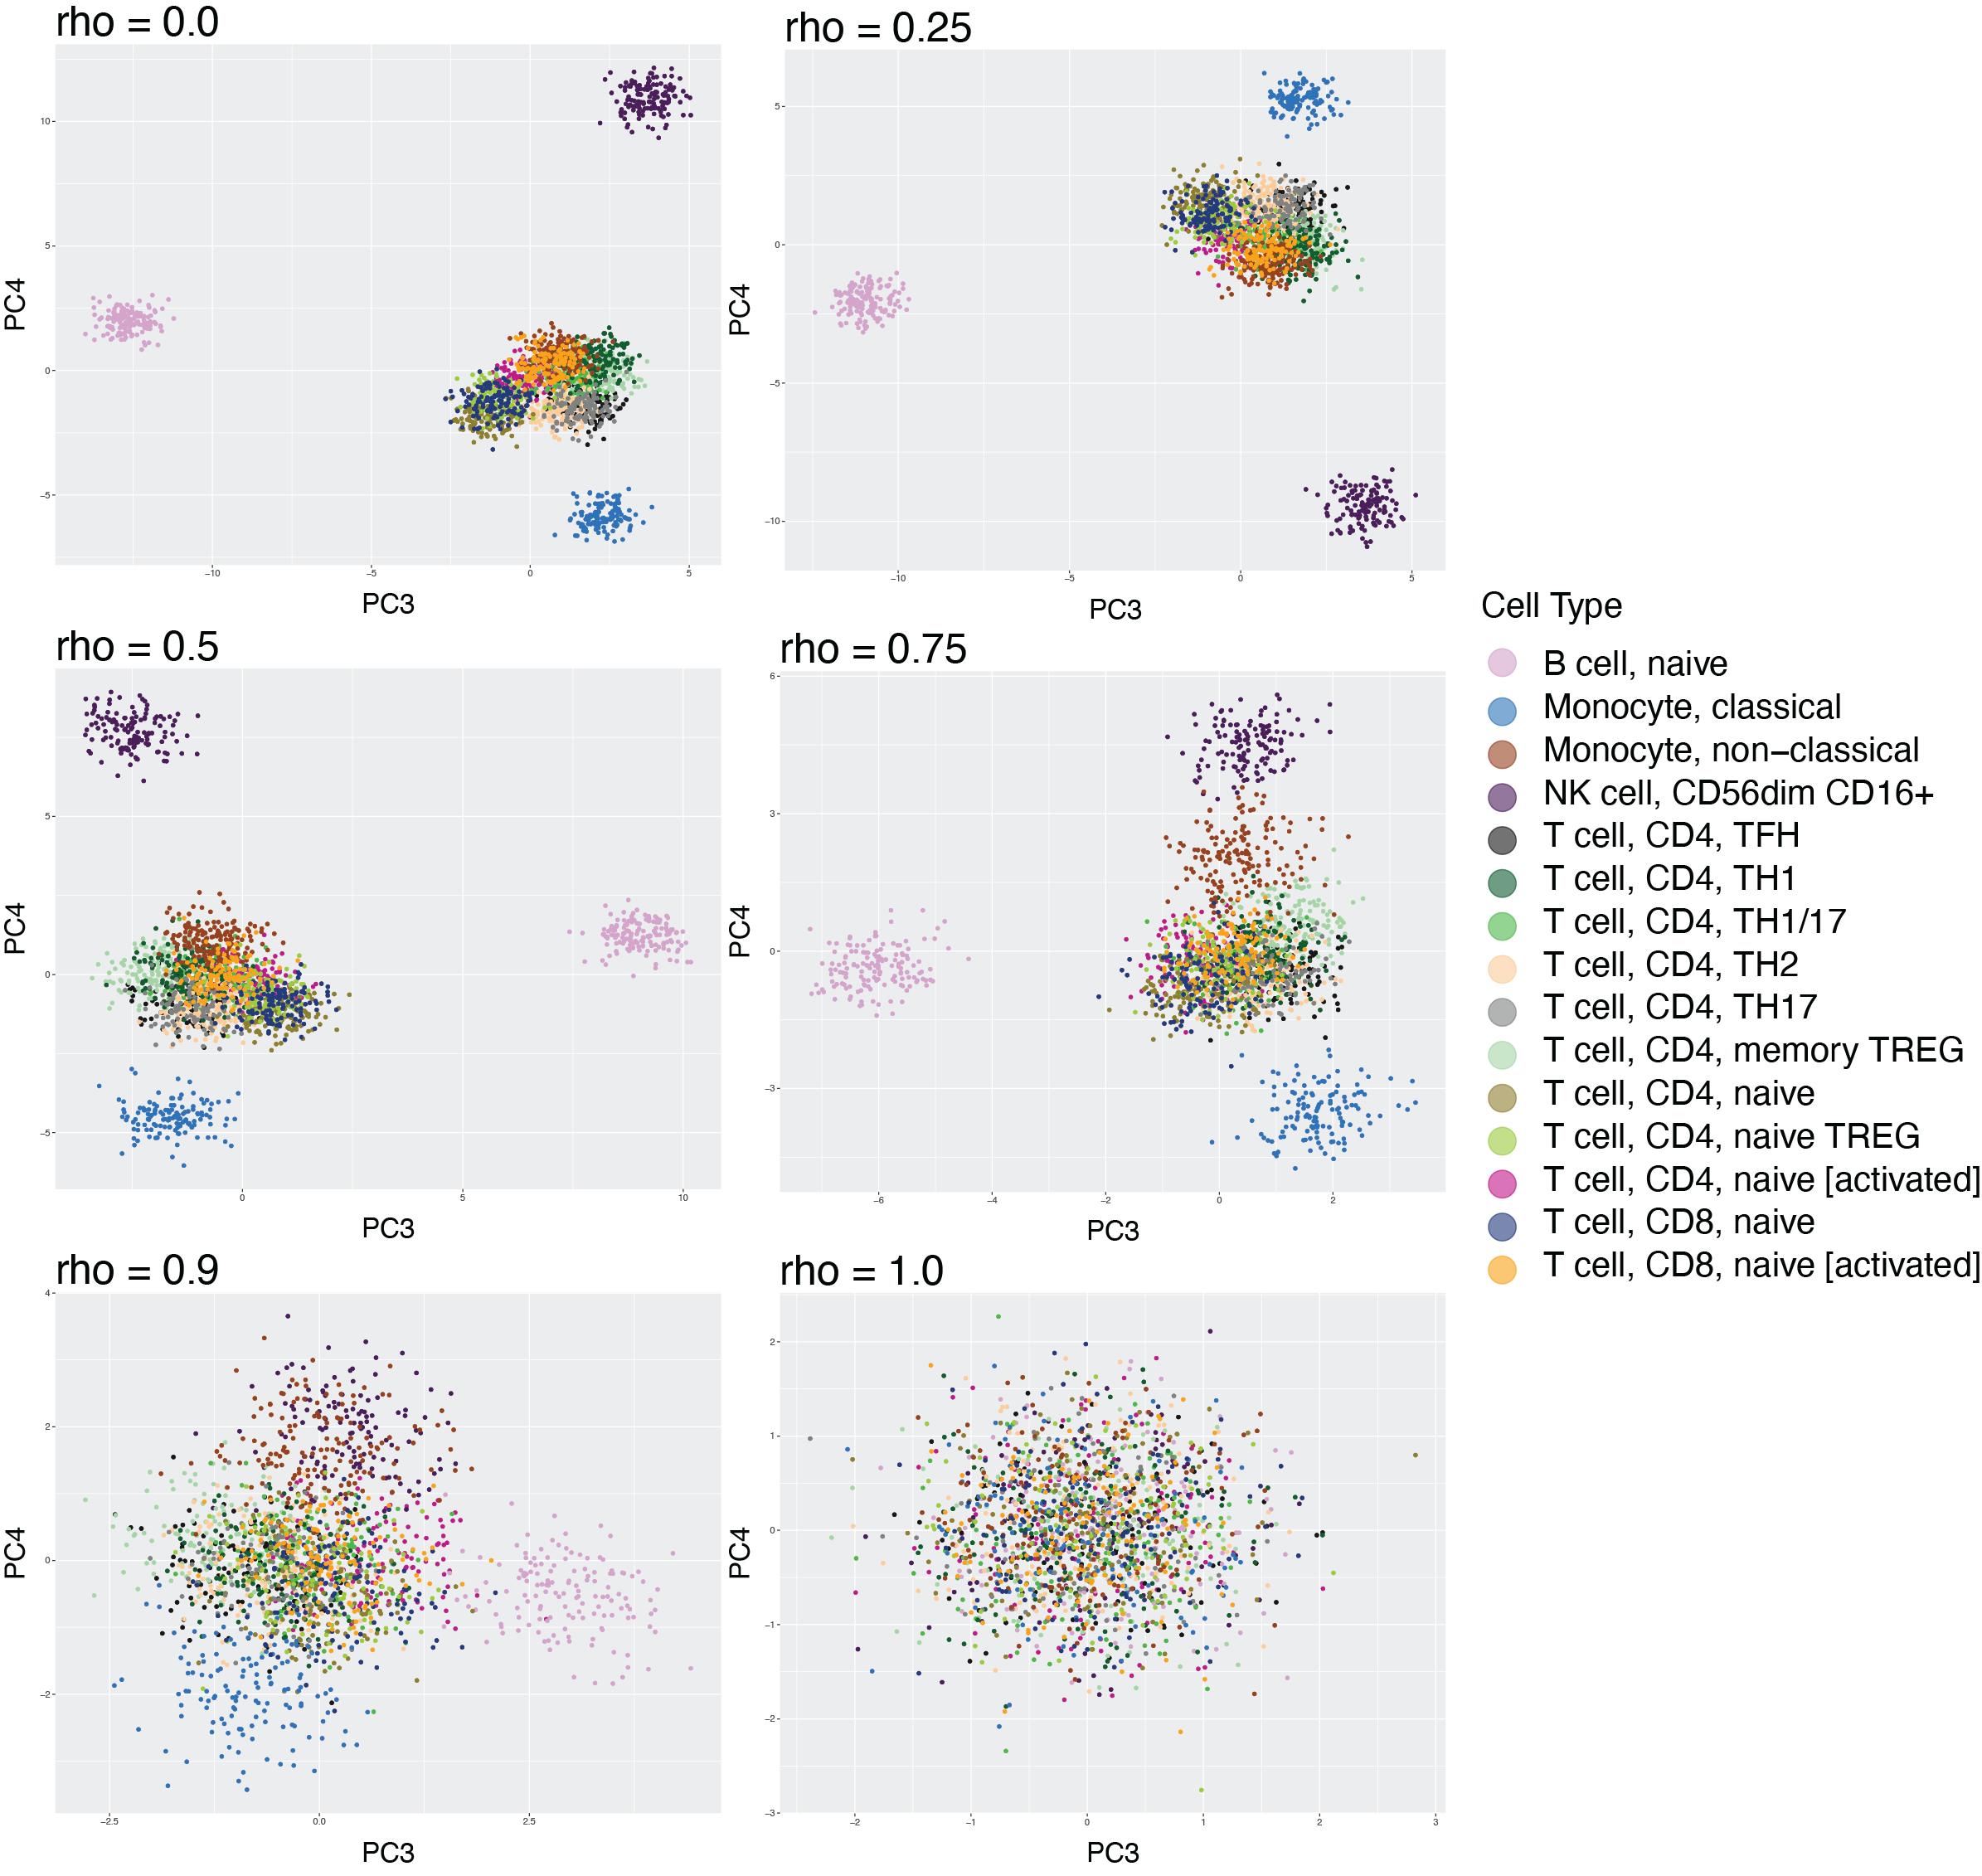
\includegraphics[width=\textwidth]{Figures/sim_data_PC34.png}
    \caption{\textbf{Simulated scRNA-seq datasets exhibit realistic distribution of expression patterns across various noise levels} Shown are the plots of third and fourth PCs for generated immune cell scRNA-seq datasets from the simulation scheme. Datasets generated using various noise proportions $\rho = \{0.0, 0.25, 0.5, 0.75, 0.9, 1.0\}$ are shown and coloured by cell type.}
    \label{fig:ct-pca-supp}
\end{figure}
\renewcommand{\arraystretch}{1}
\begin{table}[]
    \centering
    \begin{tabular}{|p{3cm}||p{4cm}|p{4cm}|}
    \hline
    Node & No. significantly upregulated genes & No. significantly downregulated genes\\
    \hline
    \multicolumn{3}{|c|}{Level 0}\\
    \hline
        \texttt{node\_0} & 0 & 157 \\
    \hline
    \multicolumn{3}{|c|}{Level 1}\\
    \hline
        \texttt{node\_1} & 525 & 242 \\        \texttt{node\_2} & 133 & 100 \\
    \hline
    \multicolumn{3}{|c|}{Level 2}\\
    \hline
        \texttt{node\_3} & 215 & 71 \\
        \texttt{node\_4} & 198 & 69 \\
        \texttt{node\_5} & 1705 & 289 \\
        \texttt{node\_6} & 485 & 123 \\
    \hline
    \multicolumn{3}{|c|}{Level 3}\\
    \hline
        \texttt{node\_7} & 1399 & 102 \\
        \texttt{node\_8} & 47 & 6 \\
        \texttt{node\_9} & 227 & 29 \\
        \texttt{node\_10} & 361 & 54 \\
        \texttt{node\_11} & 582 & 54 \\
        \texttt{node\_12} & 1451 & 160 \\
        \texttt{node\_13} & 677 & 74 \\
        \texttt{node\_14} & 280 & 63 \\
    \hline
    \multicolumn{3}{|c|}{Level 4}\\
    \hline
        \texttt{node\_15} & 830 & 16 \\
        \texttt{node\_16} & 823 & 56 \\
        \texttt{node\_17} & 41 & 3 \\
        \texttt{node\_18} & 49 & 2 \\
        \texttt{node\_19} & 1172 & 93 \\
        \texttt{node\_20} & 334 & 19 \\
        \texttt{node\_21} & 486 & 33 \\
        \texttt{node\_22} & 913 & 81 \\
        \texttt{node\_23} & 808 & 43 \\
        \texttt{node\_24} & 1185 & 100 \\
        \texttt{node\_25} & 764 & 59 \\
        \texttt{node\_26} & 1003 & 74 \\
        \texttt{node\_27} & 1096 & 102 \\
        \texttt{node\_28} & 894 & 44 \\
        \texttt{node\_29} & 286 & 7 \\
        \texttt{node\_30} & 638 & 87 \\
    \hline
    \end{tabular}
    \caption{\textbf{Table outlining the number of significant genes for each latent node} Upregulated genes are identified as genes with an embedding value of $\hat{\beta} > 0$ to a significance level of $\alpha = 0.05$. Inversely, downregulated genes are those with an embedding values of $\hat{\beta} < 0$. }
    \label{tab:sig_genes}
\end{table}

\begin{table}[]
    \centering
    \begin{tabular}{|p{3cm}||p{4cm}|p{4cm}|}
    \hline
    Node & No. unique significantly upregulated genes & No. unique significantly downregulated genes\\
    \hline
    \multicolumn{3}{|c|}{Level 0}\\
    \hline
        \texttt{node\_0} & 0 & 157 \\
    \hline
    \multicolumn{3}{|c|}{Level 1}\\
    \hline
        \texttt{node\_1} & 525 & 154 \\        \texttt{node\_2} & 133 & 40 \\
    \hline
    \multicolumn{3}{|c|}{Level 2}\\
    \hline
        \texttt{node\_3} & 188 & 19 \\
        \texttt{node\_4} & 183 & 19 \\
        \texttt{node\_5} & 1662 & 250 \\
        \texttt{node\_6} & 476 & 78 \\
    \hline
    \multicolumn{3}{|c|}{Level 3}\\
    \hline
        \texttt{node\_7} & 1394 & 88 \\
        \texttt{node\_8} & 38 & 1 \\
        \texttt{node\_9} & 213 & 14 \\
        \texttt{node\_10} & 344 & 17 \\
        \texttt{node\_11} & 292 & 31 \\
        \texttt{node\_12} & 995 & 41 \\
        \texttt{node\_13} & 622 & 26 \\
        \texttt{node\_14} & 249 & 26 \\
    \hline
    \multicolumn{3}{|c|}{Level 4}\\
    \hline
        \texttt{node\_15} & 429 & 12 \\
        \texttt{node\_16} & 620 & 8 \\
        \texttt{node\_17} & 37 & 1 \\
        \texttt{node\_18} & 45 & 1 \\
        \texttt{node\_19} & 1098 & 69 \\
        \texttt{node\_20} & 244 & 12 \\
        \texttt{node\_21} & 400 & 19 \\
        \texttt{node\_22} & 870 & 49 \\
        \texttt{node\_23} & 639 & 34 \\
        \texttt{node\_24} & 1022 & 61 \\
        \texttt{node\_25} & 214 & 22 \\
        \texttt{node\_26} & 445 & 24 \\
        \texttt{node\_27} & 959 & 49 \\
        \texttt{node\_28} & 687 & 30 \\
        \texttt{node\_29} & 229 & 5 \\
        \texttt{node\_30} & 608 & 44 \\
    \hline
    \end{tabular}
    \caption{\textbf{Table outlining the number of unique significant genes for each latent node} Upregulated genes are identified as genes with an embedding value of $\hat{\beta} > 0$ to a significance level of $\alpha = 0.05$. Inversely, downregulated genes are those with an embedding values of $\hat{\beta} < 0$. Genes are considered unique to a node if it does not also appear as a significant gene in its parent and sibling node.}
    \label{tab:unique_sig_genes}
\end{table}

\begin{figure}
    \centering
    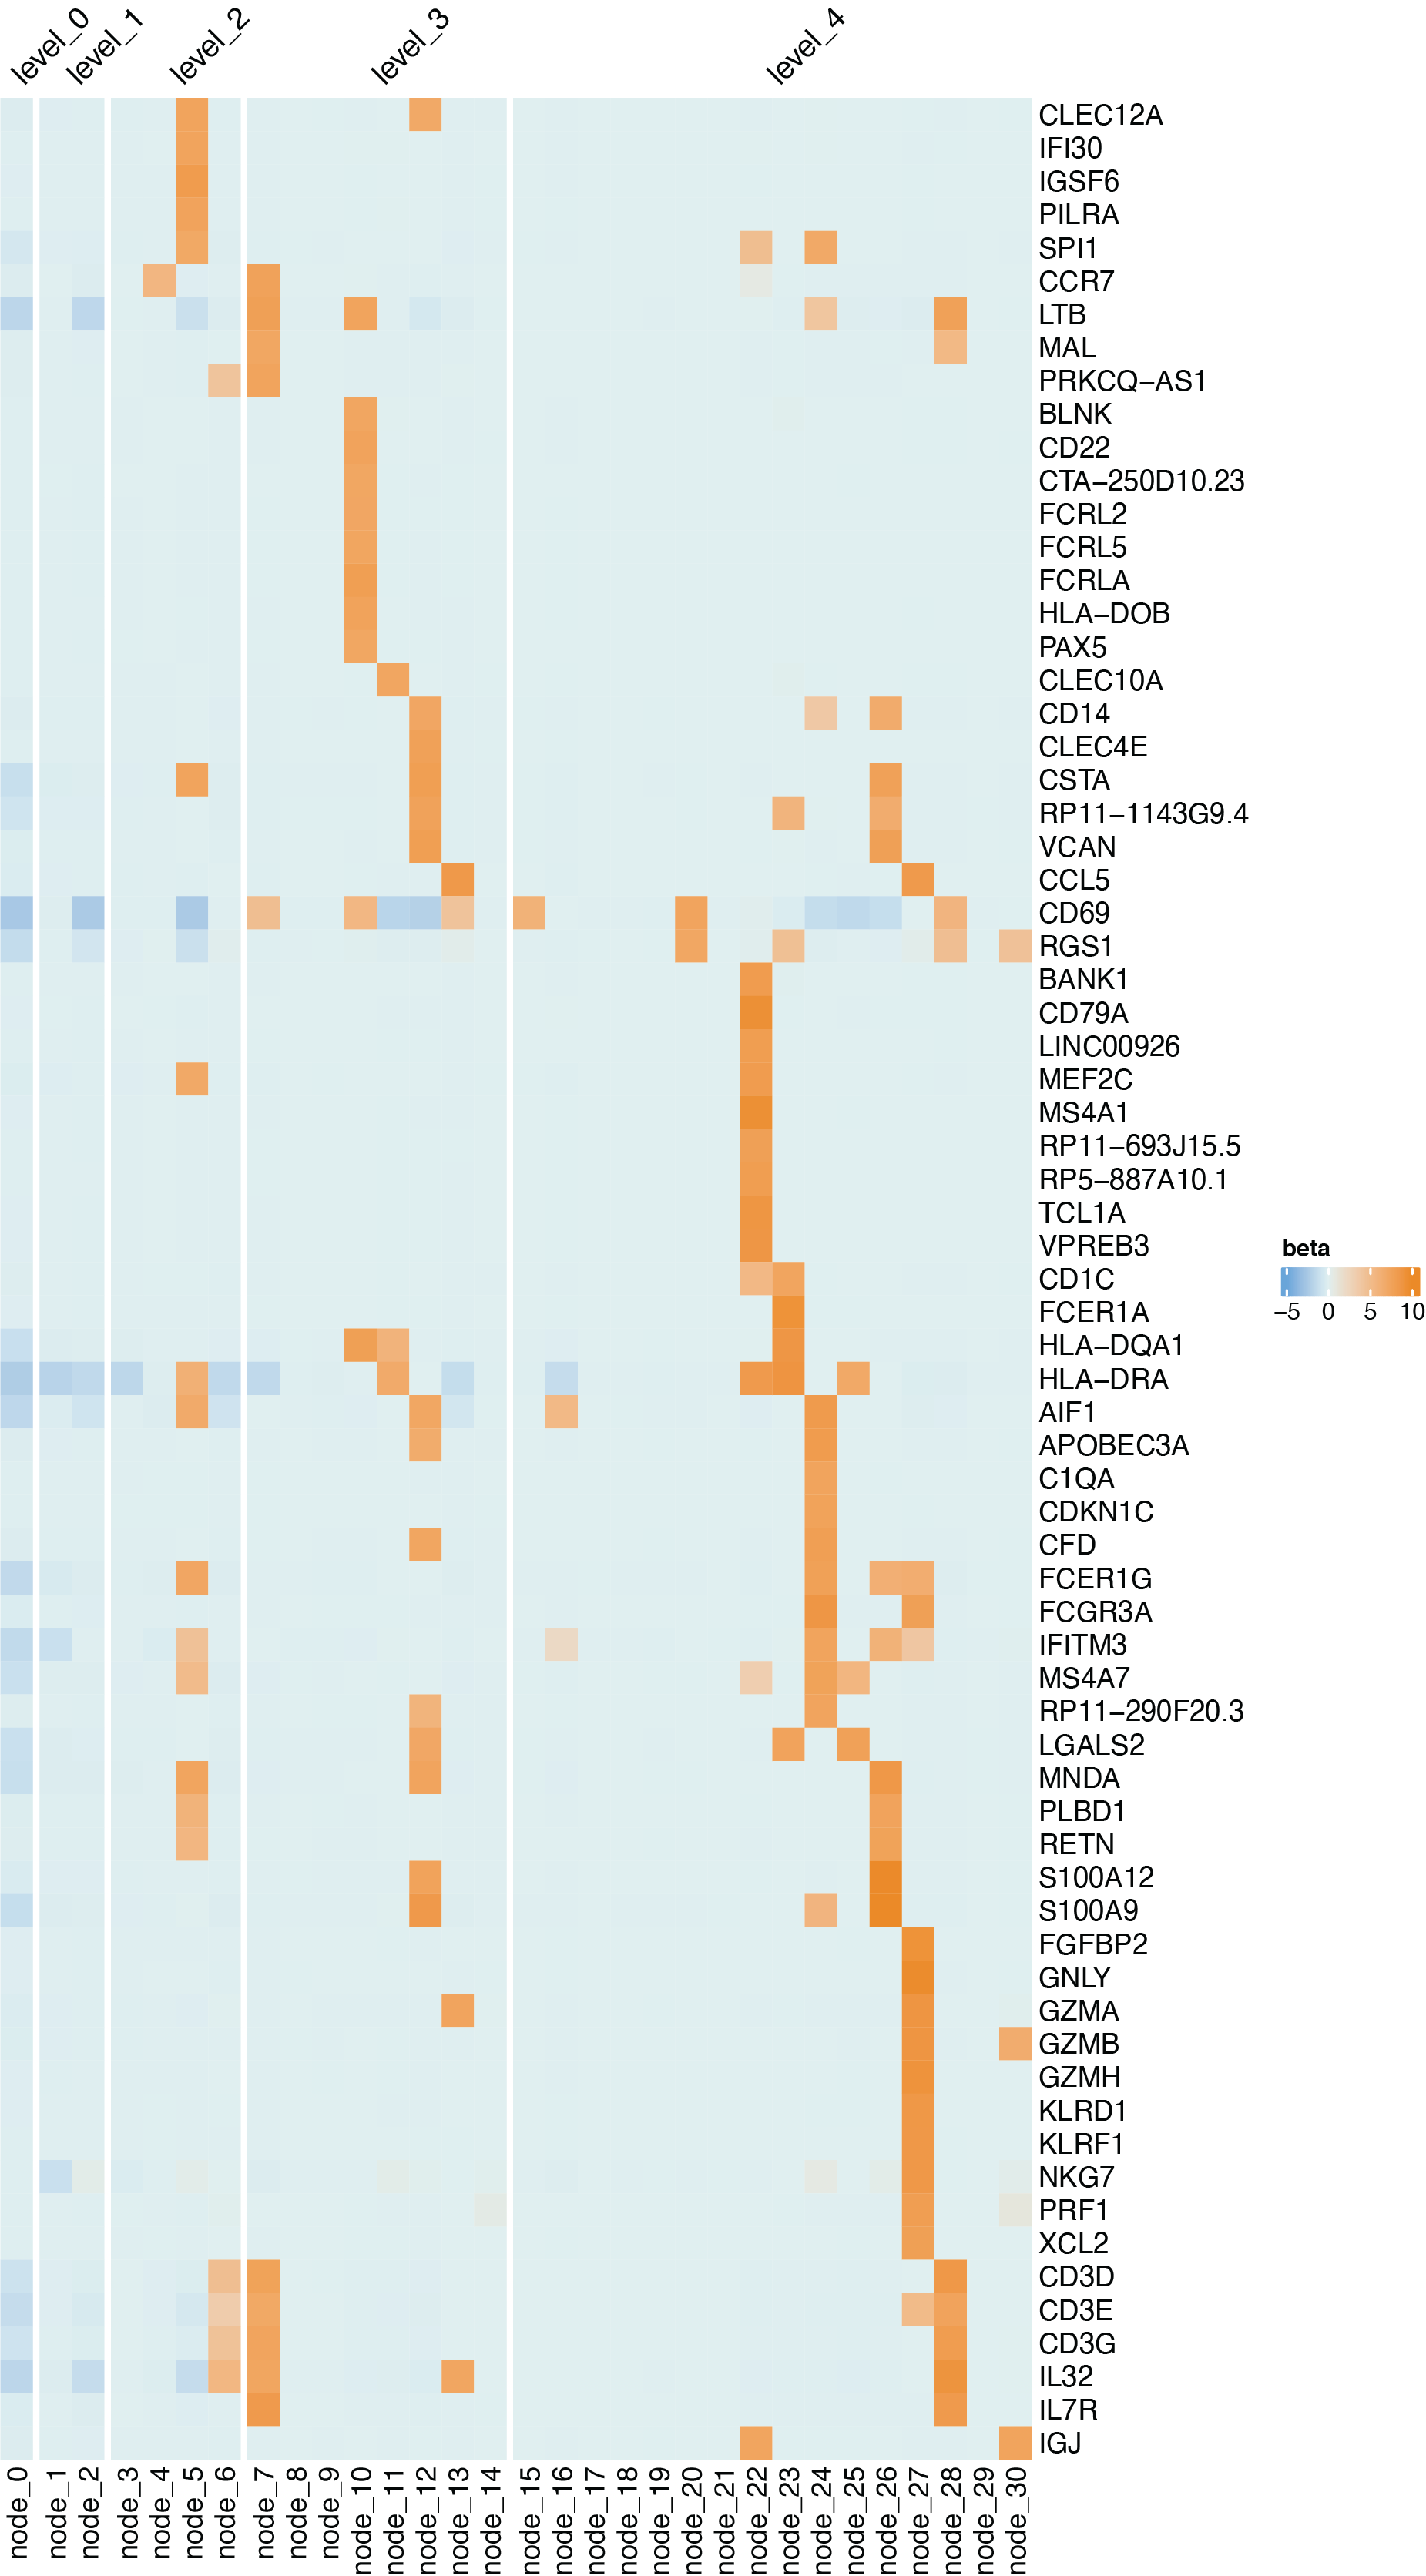
\includegraphics[scale=0.6]{Figures/top_beta_hm.png}
    \caption{\textbf{Heatmap of top genes shows candidates for further analysis} Heatmap shows estimated gene embedding values $\hat{\beta}$ of top genes across all latent tree nodes. Genes are selected as the 80 gene with the greatest absolute $\hat{\beta}$ values amongst the aggregated pool of the top ten genes per latent tree node.}
    \label{fig:top_beta_hm}
\end{figure}

\begin{figure}
    \centering
    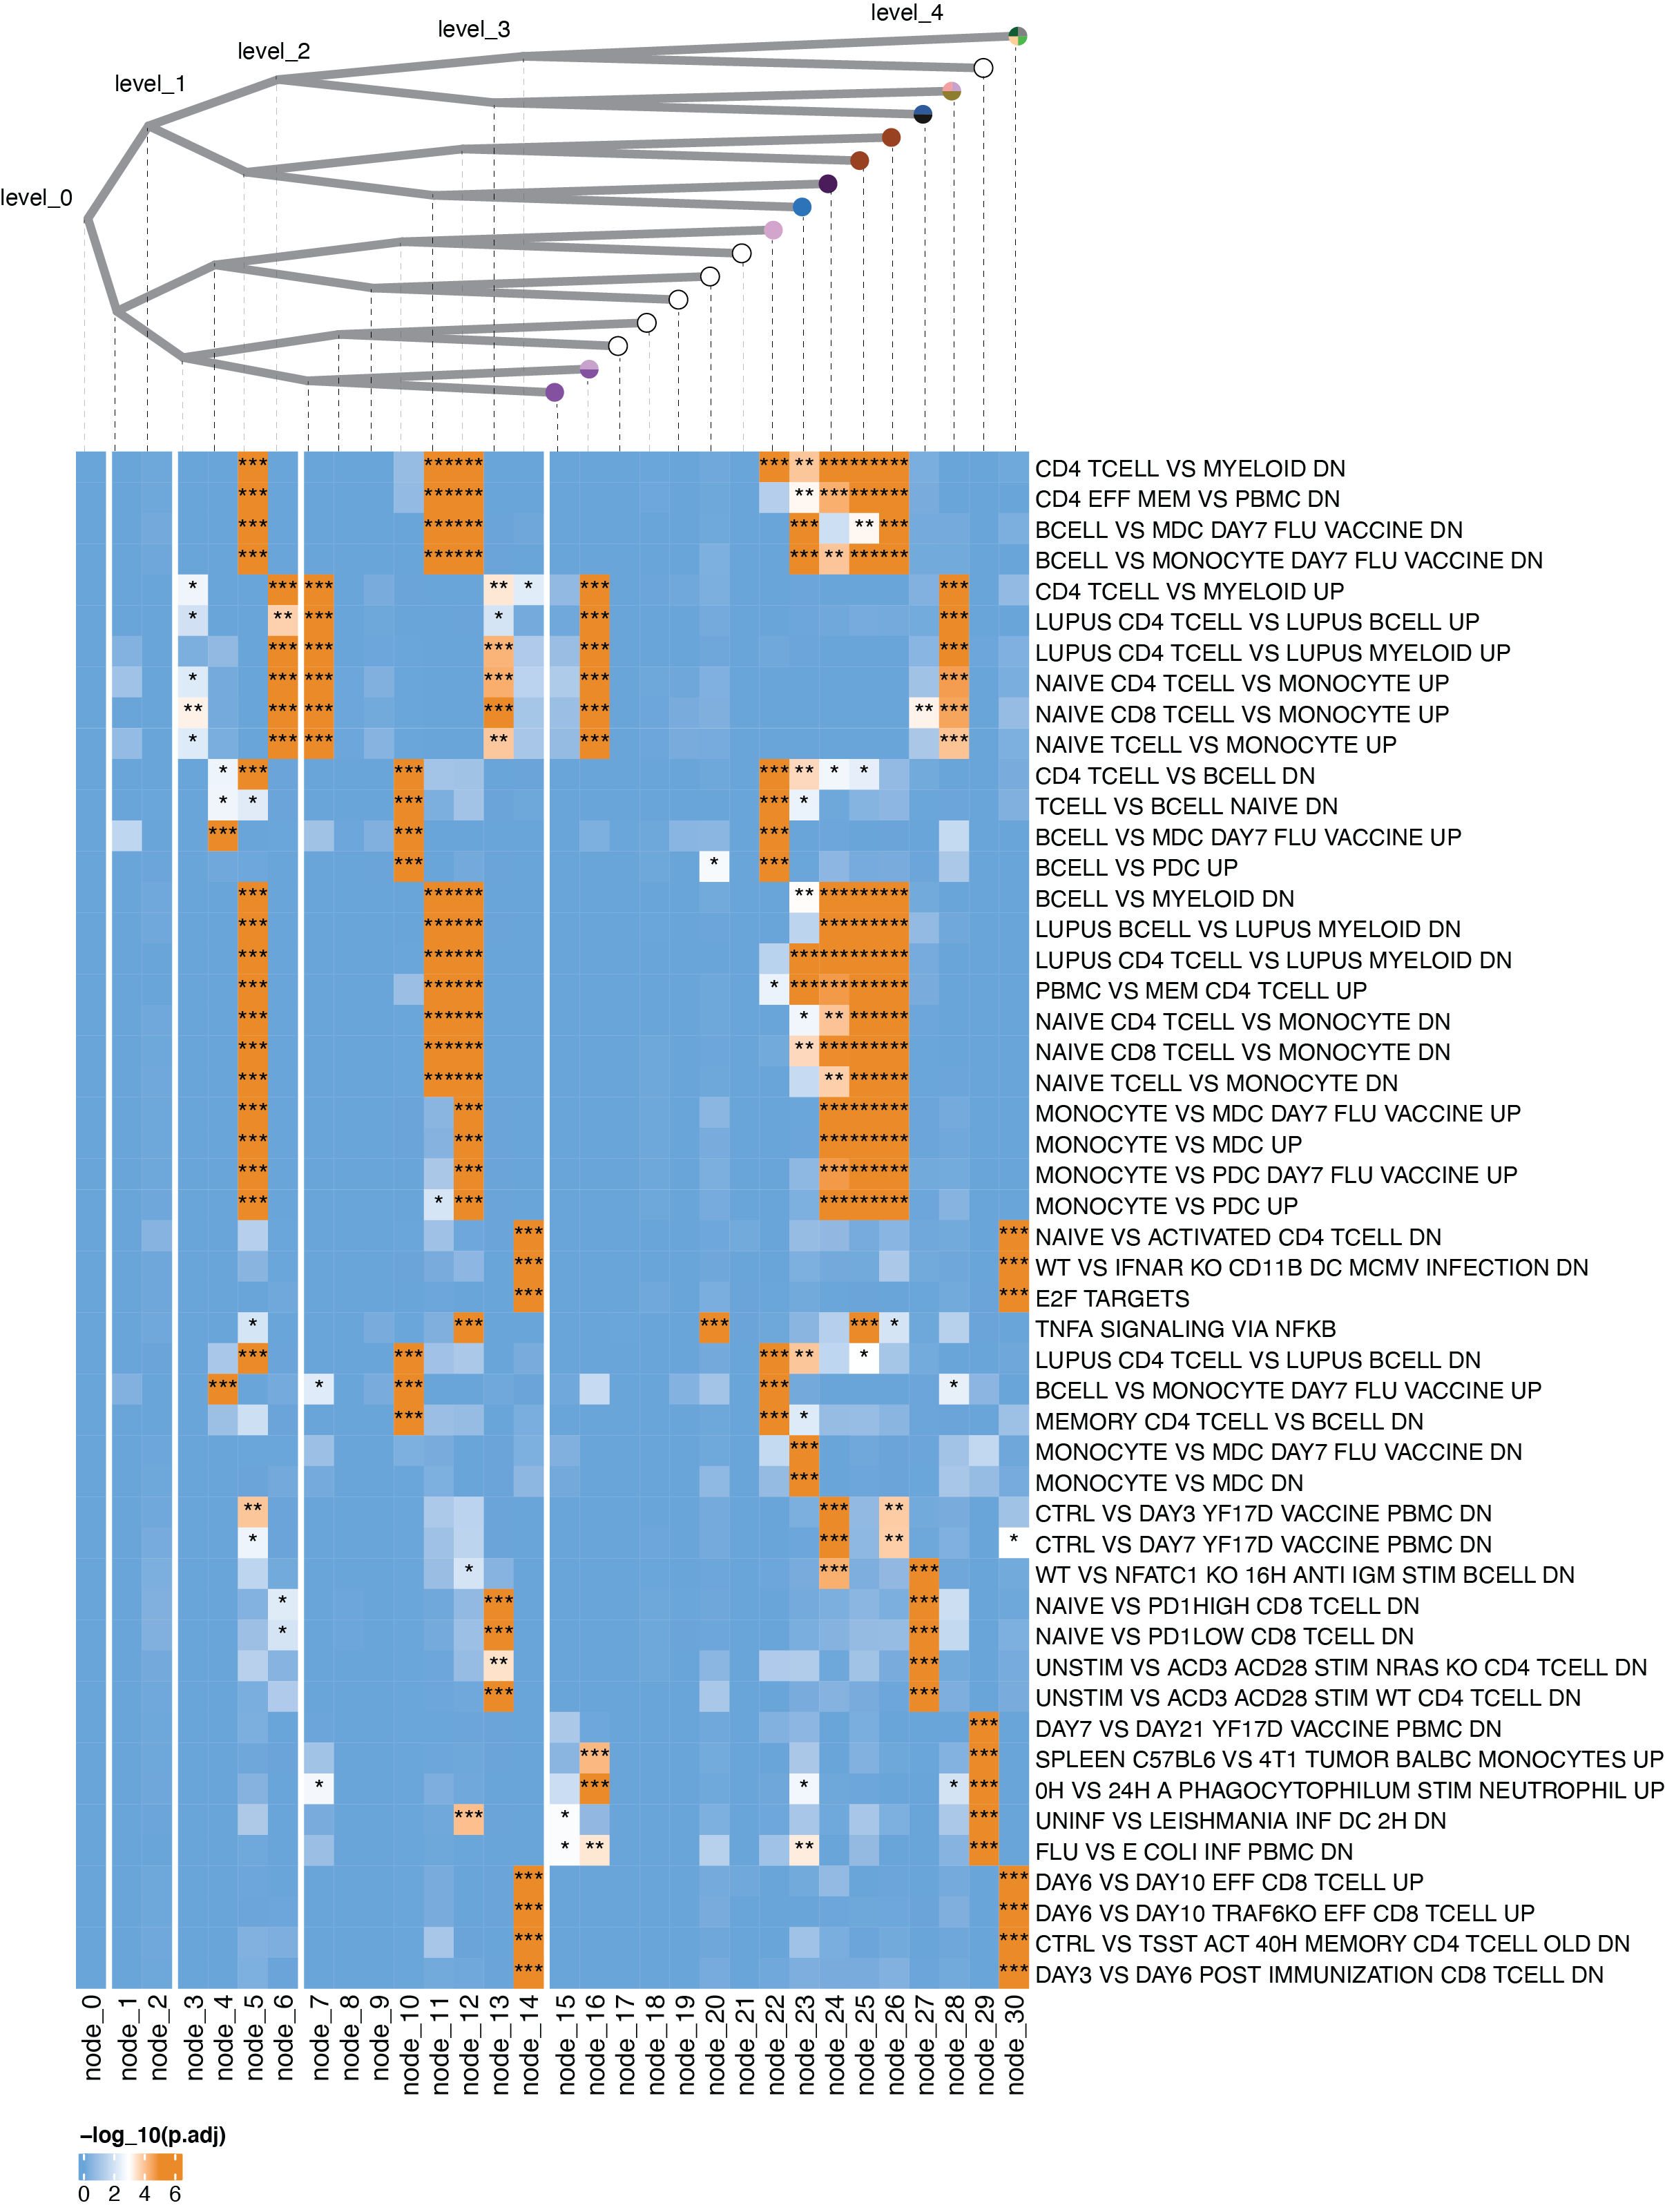
\includegraphics[scale=0.65]{Figures/immune_gsea.png}
    \caption{\textbf{Enrichment analysis of gene sets related to immune function show cell function described by latent node embeddings} Heatmap shows the $-\log(p)$ enrichment significance of each gene set per node. Significance annotations are as follows: $*** - p < 0.0001, ** - p < 0.001, * - p < 0.01$}
    \label{fig:immune_gsea}
\end{figure}


\chapter{Materials and Methods for \textit{in vitro} Experiments}
\section{CD4+ T Cell isolation}
\label{cha:cd4diff}
For \textit{in vitro} cell culture, male wild-type BL6 mice were bred and kept in specific pathogen-free (SPF) conditions at the Centre for Molecular Medicine and Therapeutics (CMMT) mouse facility at BC Children's Hospital Research Institute. All animals were cared for in compliance with the Canadian Council on Animal care and the University of British Columbia Animal Care Committee (Protocol numbers A19-024, A19-0273 and A21-0266). 

Spleen and lymph nodes were harvested from mice at 8-14 weeks of age. Following organ harvest, naïve CD4+ T cells were isolated by negative selection using a StemCell Mouse CD4+ T Cell Isolation Kit according to the manufacturer's protocol (StemCell Technologies, Cat: 19852). 

\section{CD4+ T Cell Subtype Polarization}
All isolated CD4+ T cells were cultured in T cell media (TCM) containing RPMI 1640 media (Corning) supplemented with 10\% fetal bovine serum (FBS) (Gibco), 2mM L-Glutamine, 100 U/mL penicillin/streptomycin, 55 $\mu$M $\beta$-Mercaptoethanol (Life Technologies). Cells were activated using 5$\mu$g/mL plate-bound anti-CD3 (BioXCell), 2 $\mu$g/mL soluble anti-CD8 (BioXCell) and 10 ng/mL recombinant human (rh) IL-2 (Peprotech) at a concentration of $1.5 \times 10^6$ cells/mL. 

In addition to the above media, Helper T cell subtypes were polarized as follows: 
\begin{itemize}
    \item T$_H$0: No additional cytokines or antibodies
    \item T$_H$1: 4 $\mu$g/mL anti-mouse IL-4 (BioXCell), 10 ng/mL recombinant murine (rm) IL-12
    \item Regulatory T cell (T$_\text{reg}$): 10 ng/mL rh TGF-$\beta$1 (Peprotech)
    \item Non-pathogenic T$_H$17: 10 ng/mL rmIL-6 (Peprotech), 5 ng/mL TGF-$\beta$1
    \item Pathogenic T$_H$17 (T$_H$17p): 10 ng/mL rmIL-6, 5 ng/mL TGF-$\beta$1, 10 ng/mL rmIL-1$\beta$ (Peprotech), 10 ng/mL rmIL-23 (BioLegend)
\end{itemize}

72-hours after initial activation, cells were split with fresh media containing the same polarization conditions with the exception anti-CD3 and anti-CD28 which were omitted. On day 4, cells were collected for downstream flow cytometry analysis. 

\section{Flow Cytometry Analysis}
Cells collected for flow cytometry analysis are spun, supernatant discarded, and resuspended in TCM supplemented with 10 ng/mL rhIL-2 and 1.5 $\mu$g/mL Brefeldin A (eBioscience). A subsample of cells were further restimulated with phorbol 12-myristate (PMA) (25 ng/mL; Sigma) and ionomycin (250 ng/mL; Sigma). Following resuspension, all samples are incubated for 4 hours before staining. 

Surface proteins are stained by resuspending cell samples in FACS buffer comprised of Phosphate Buffered Saline (PBS) (Corning), 2\% FBS, and surface marker antibody cocktail containing PerCP-Cy5.5 anti-mouse CD69 (1:200, clone: H1.2F3 BioLegend), FITC anti-mouse CD25 (1:200, clone: PC61 BioLegend), eFluor 780 Fixable Viability Dye (1:10000, eBioscience), BV785 anti-mouse CD8$\alpha$ (1:200, clone: 53-6.7, BioLegend), and BV605 anti-mouse CD4 (1:200, clone: RM4-4, BioLegend). Cells are incubated in antibody cocktail for 30 minutes at room temperature in the dark. 

To detect intracellular proteins, all samples were fixed and permeabilized using the Foxp3/Transcription Factor Staining Buffer Set (eBiosciences), followed by intracellular marker antibody cocktail containing Alexa Fluor 700 monoclonal antibody FOXP3 (1:200, clone: FJK-16s, eBiosciences), BV510 anti-mouse ROR$\gamma$t (1:200, clone: Q31-378), BV421 anti-T-bet (1:200, clone: 4B10, BioLegend), APC anti-mouse IL-17A (1:200, clone: TC11-18H10.1, BioLegend), and PE IFN-$\gamma$ (1:200, clone: XMG1.2, BioLegend). Cells are incubated for 60 minutes at room temperature in the dark. Sample were resuspended in FACS buffer and FACS data was acquired with a BD LSRFortessa X-20 flow cytometer. FlowJo software was used for analysis. 


%% This changes the headings and chapter titles (no numbers for
%% example).
\backmatter

%% Indices come here if you have them.

\end{document}
\endinput
%%
%% End of file `ubcsample.tex'.
